\chapter{Anhang}
\label{ch:chapter07}

\begin{sloppypar}

\section{Referenzmessung (Alter Scheduler)}

\subsection{Ein Thread}
\begin{figure}[H]
\centering
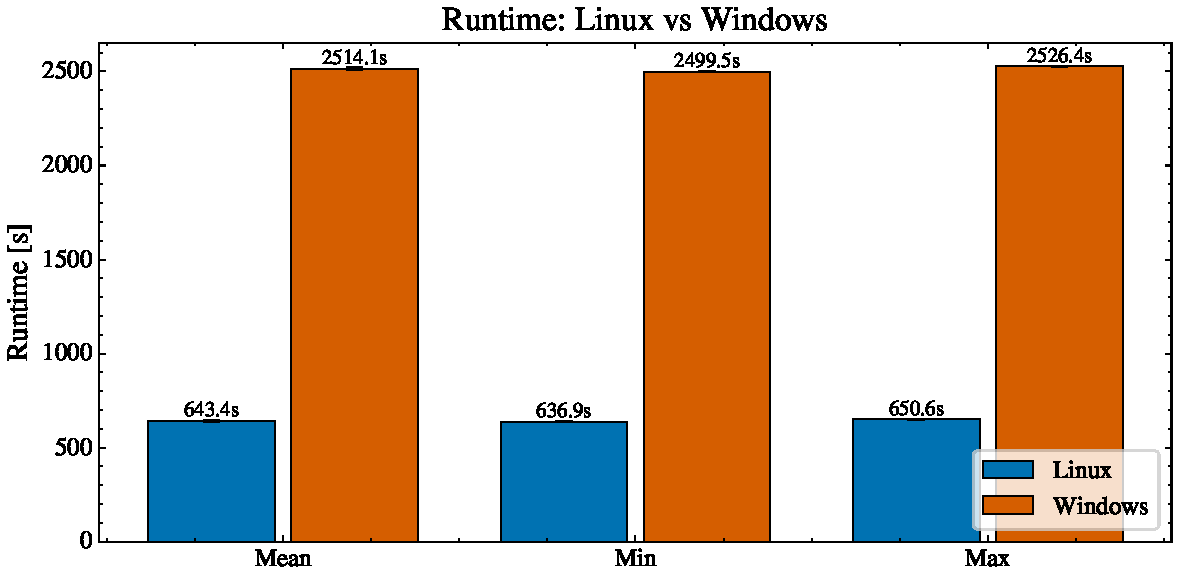
\includegraphics[width=\textwidth]{Messungen/OLD_1T/runtime_bars_combined.pdf}
\caption{Laufzeiten der Referenzmessung auf Linux und Windows bei einem Thread, dargestellt als Balkendiagramm mit Mittelwerten und Standardabweichungen aus 20 Messläufen}
\label{fig:ref-1t-runtime}
\end{figure}

\begin{figure}[H]
\centering
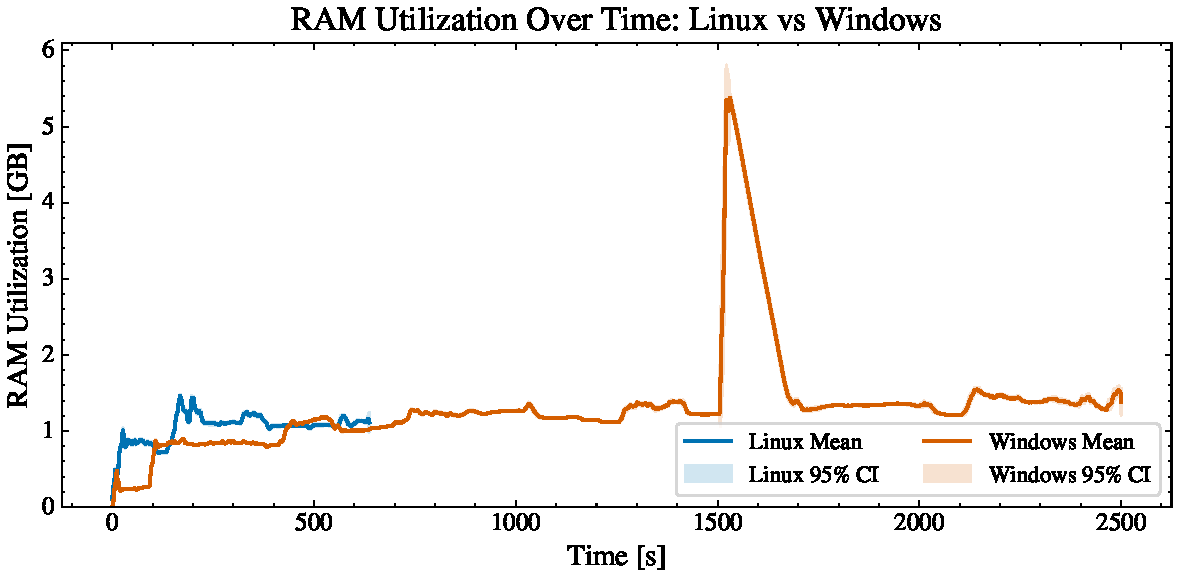
\includegraphics[width=\textwidth]{Messungen/OLD_1T/ram_timeseries_combined.pdf}
\caption{Zeitlicher Verlauf der \acs{RAM}-Auslastung der Referenzmessung auf Linux und Windows bei einem Thread}
\label{fig:ref-1t-ram-ts}
\end{figure}

\begin{figure}[H]
\centering
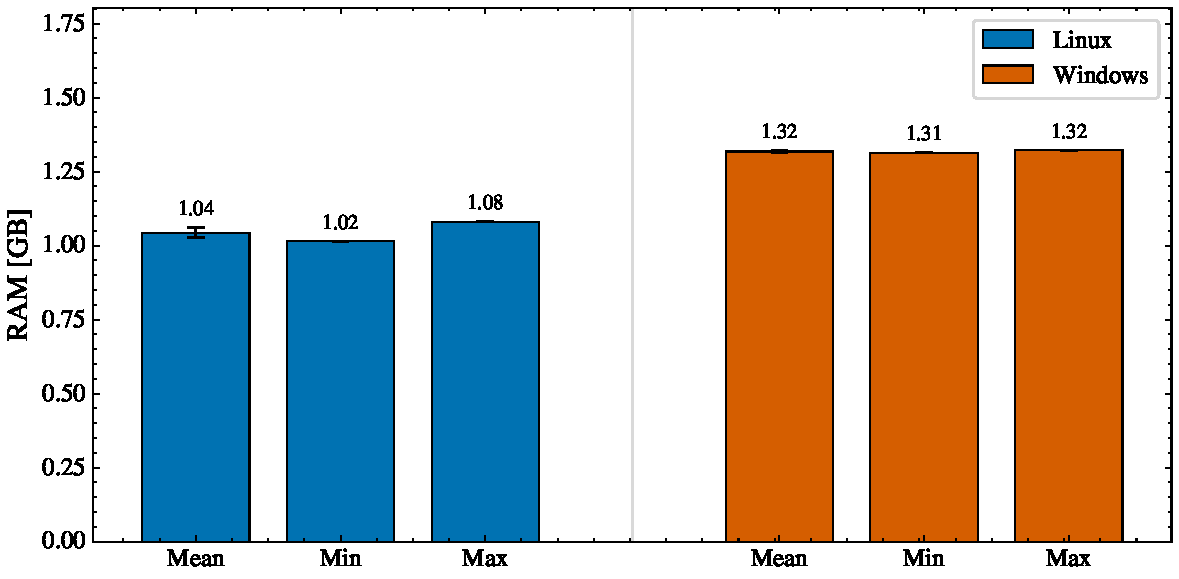
\includegraphics[width=\textwidth]{Messungen/OLD_1T/ram_bars_combined.pdf}
\caption{\acs{RAM}-Auslastung der Referenzmessung auf Linux und Windows bei einem Thread, dargestellt als Balkendiagramm mit Mittelwerten und Standardabweichungen aus 20 Messläufen}
\label{fig:ref-1t-ram}
\end{figure}

\begin{figure}[H]
\centering
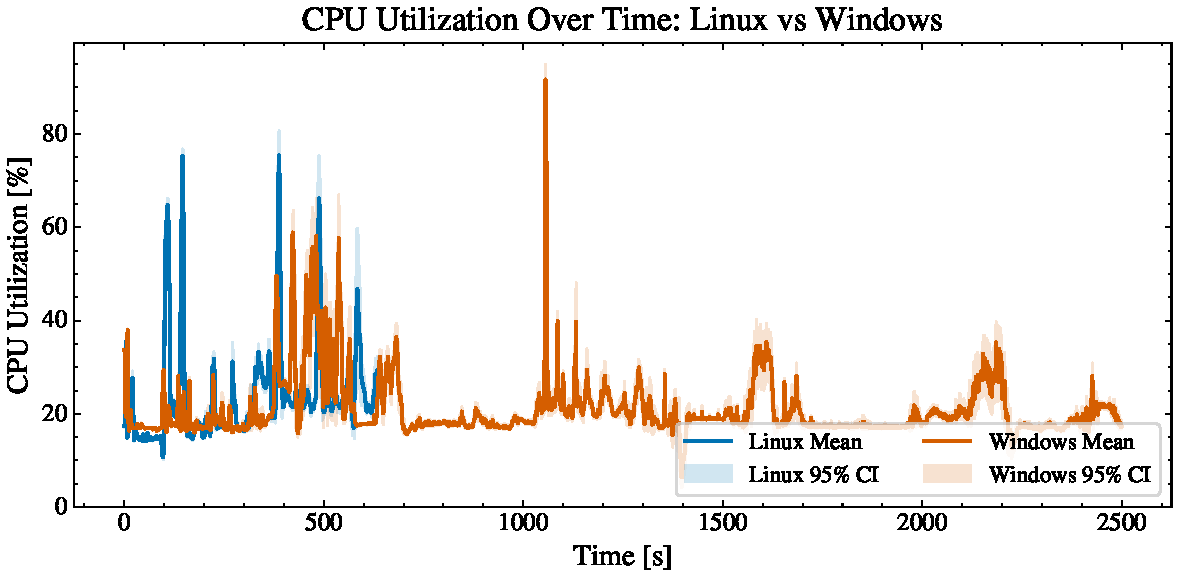
\includegraphics[width=\textwidth]{Messungen/OLD_1T/cpu_timeseries_combined.pdf}
\caption{Zeitlicher Verlauf der \acs{CPU}-Auslastung der Referenzmessung auf Linux und Windows bei einem Thread}
\label{fig:ref-1t-cpu-ts}
\end{figure}

\begin{figure}[H]
\centering
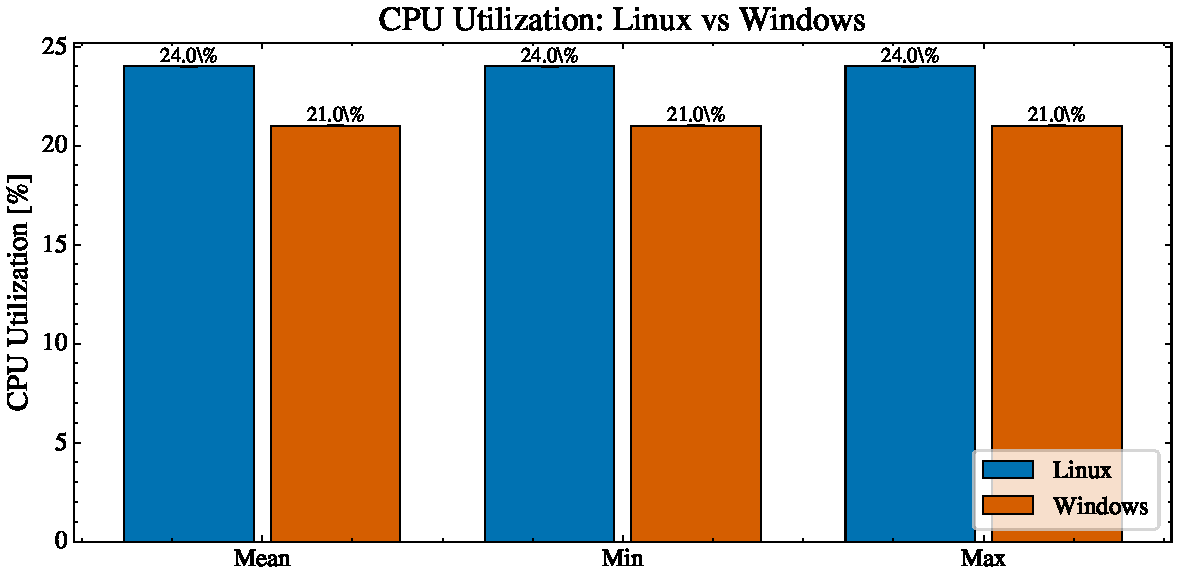
\includegraphics[width=\textwidth]{Messungen/OLD_1T/cpu_bars_combined.pdf}
\caption{\acs{CPU}-Auslastung der Referenzmessung auf Linux und Windows bei einem Thread, dargestellt als Balkendiagramm mit Mittelwerten und Standardabweichungen aus 20 Messläufen}
\label{fig:ref-1t-cpu}
\end{figure}

\subsection{Vier Threads}
\begin{figure}[H]
\centering
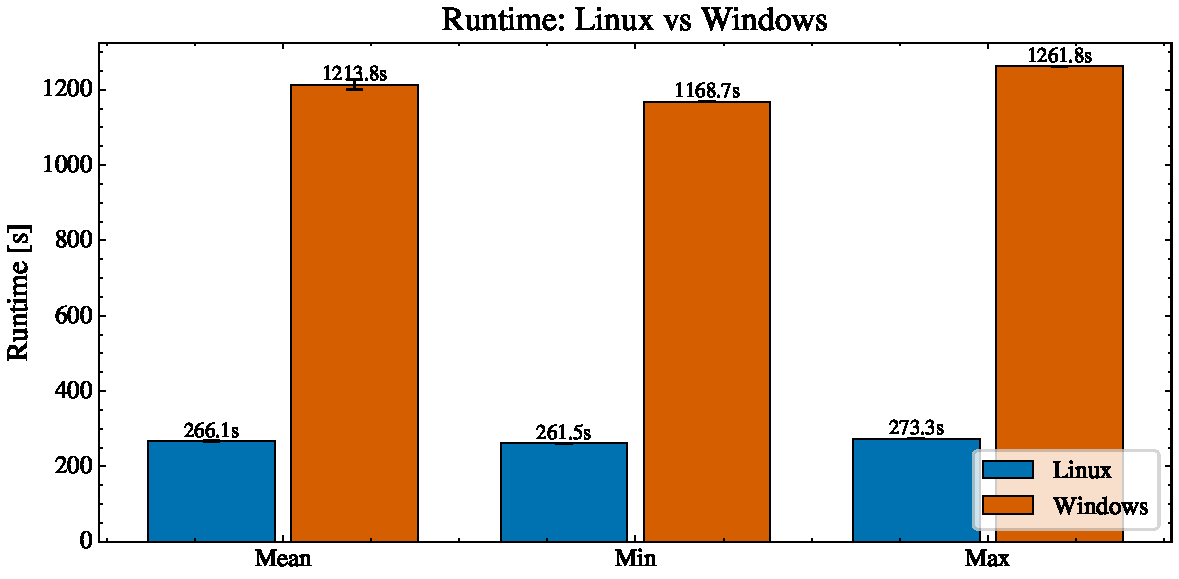
\includegraphics[width=\textwidth]{Messungen/OLD_4T/runtime_bars_combined.pdf}
\caption{Laufzeiten der Referenzmessung auf Linux und Windows bei vier Threads, dargestellt als Balkendiagramm mit Mittelwerten und Standardabweichungen aus 20 Messläufen}
\label{fig:ref-4t-runtime}
\end{figure}

\begin{figure}[H]
\centering
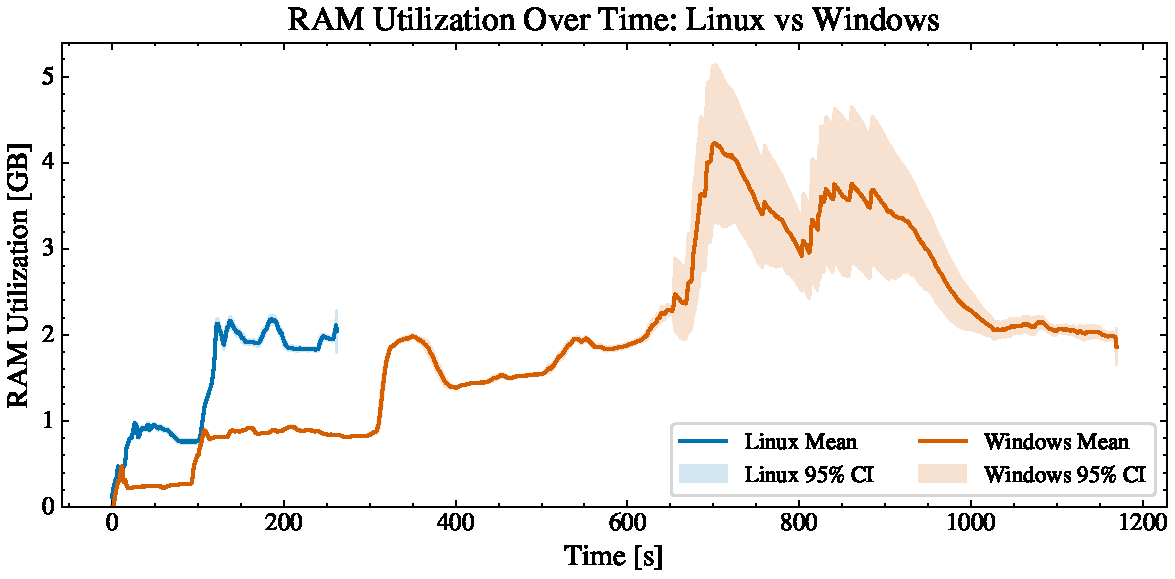
\includegraphics[width=\textwidth]{Messungen/OLD_4T/ram_timeseries_combined.pdf}
\caption{Zeitlicher Verlauf der \acs{RAM}-Auslastung der Referenzmessung auf Linux und Windows bei vier Threads}
\label{fig:ref-4t-ram-ts}
\end{figure}

\begin{figure}[H]
\centering
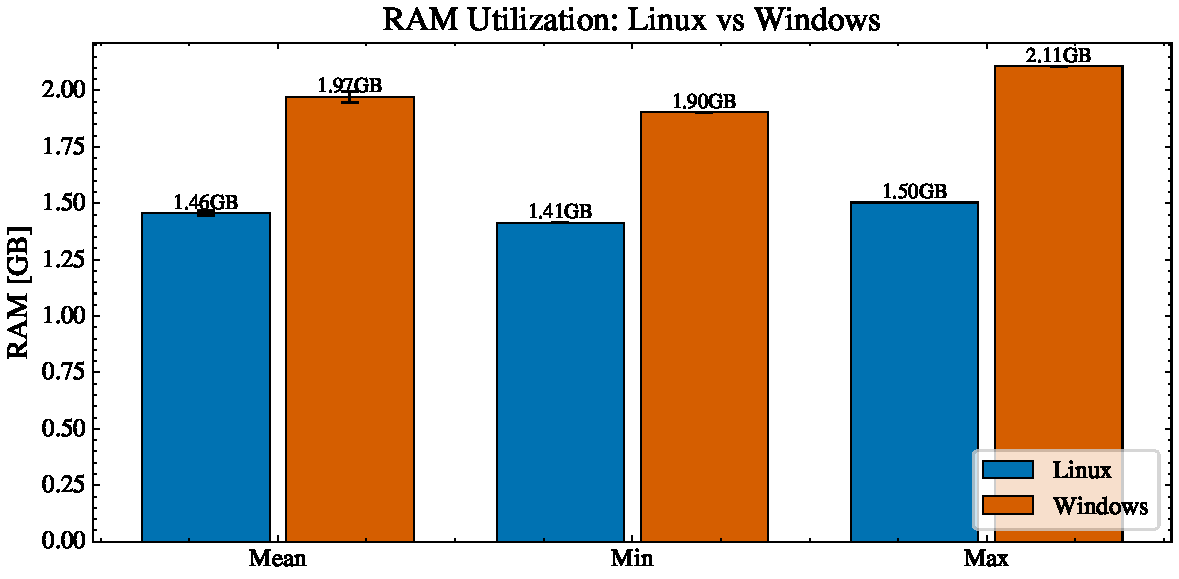
\includegraphics[width=\textwidth]{Messungen/OLD_4T/ram_bars_combined.pdf}
\caption{\acs{RAM}-Auslastung der Referenzmessung auf Linux und Windows bei vier Threads, dargestellt als Balkendiagramm mit Mittelwerten und Standardabweichungen aus 20 Messläufen}
\label{fig:ref-4t-ram}
\end{figure}

\begin{figure}[H]
\centering
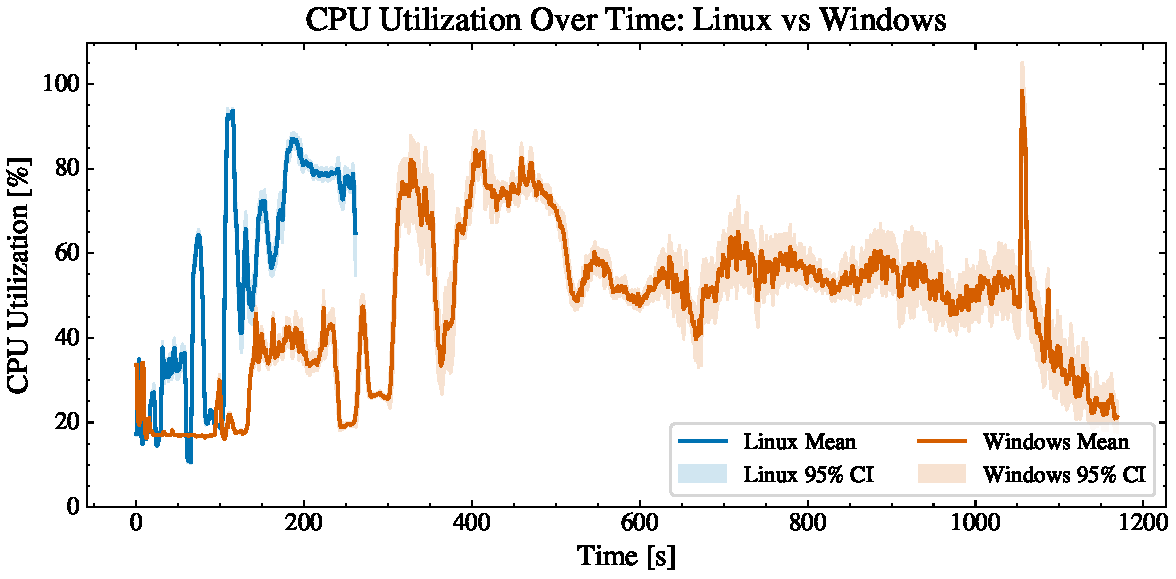
\includegraphics[width=\textwidth]{Messungen/OLD_4T/cpu_timeseries_combined.pdf}
\caption{Zeitlicher Verlauf der \acs{CPU}-Auslastung der Referenzmessung auf Linux und Windows bei vier Threads}
\label{fig:ref-4t-cpu-ts}
\end{figure}

\begin{figure}[H]
\centering
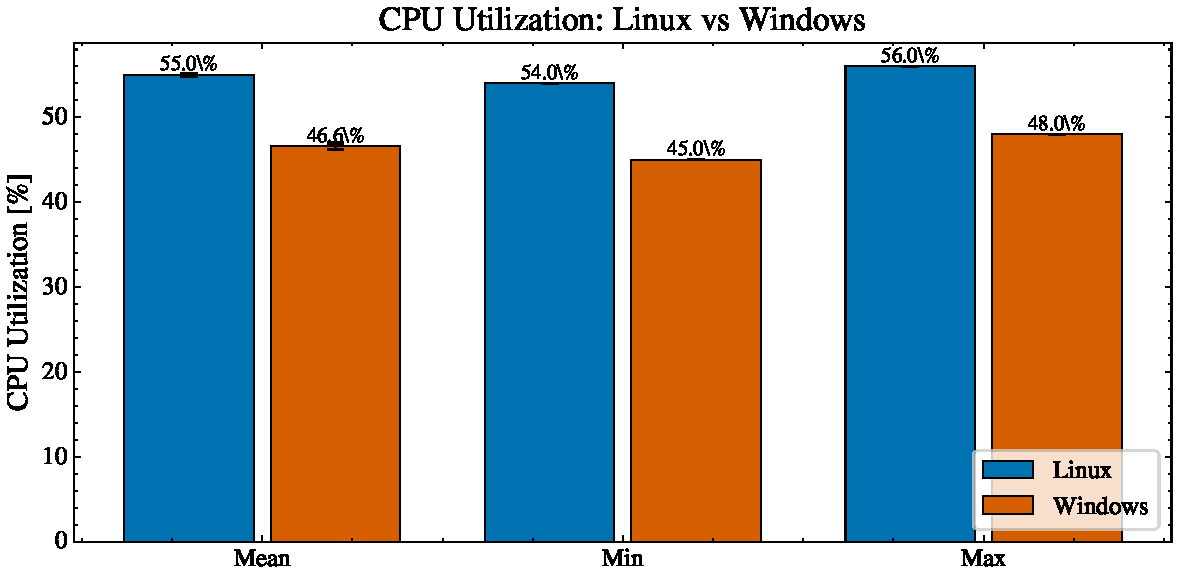
\includegraphics[width=\textwidth]{Messungen/OLD_4T/cpu_bars_combined.pdf}
\caption{\acs{CPU}-Auslastung der Referenzmessung auf Linux und Windows bei vier Threads, dargestellt als Balkendiagramm mit Mittelwerten und Standardabweichungen aus 20 Messläufen}
\label{fig:ref-4t-cpu}
\end{figure}

\subsection{Zehn Threads}
\begin{figure}[H]
\centering
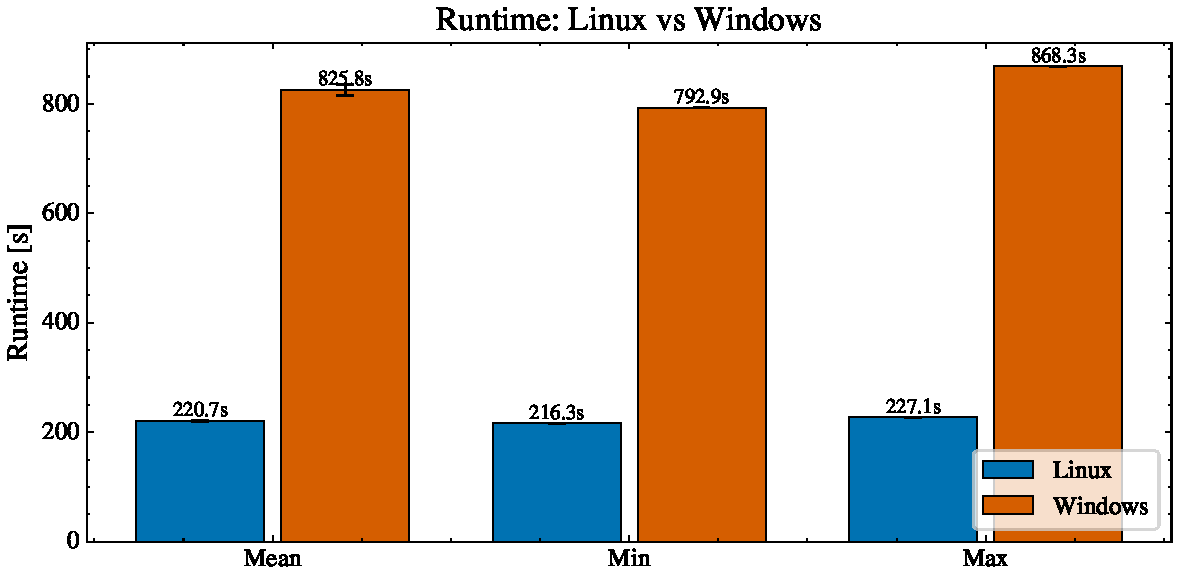
\includegraphics[width=\textwidth]{Messungen/OLD_10T/runtime_bars_combined.pdf}
\caption{Laufzeiten der Referenzmessung auf Linux und Windows bei zehn Threads, dargestellt als Balkendiagramm mit Mittelwerten und Standardabweichungen aus 20 Messläufen}
\label{fig:ref-10t-runtime}
\end{figure}

\begin{figure}[H]
\centering
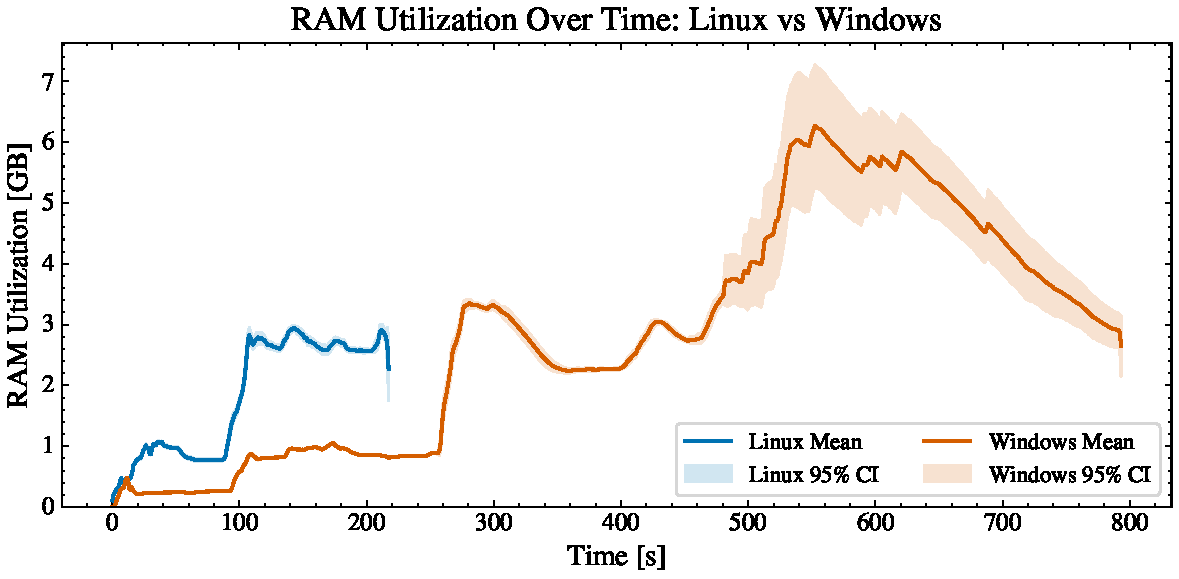
\includegraphics[width=\textwidth]{Messungen/OLD_10T/ram_timeseries_combined.pdf}
\caption{Zeitlicher Verlauf der \acs{RAM}-Auslastung der Referenzmessung auf Linux und Windows bei zehn Threads}
\label{fig:ref-10t-ram-ts}
\end{figure}

\begin{figure}[H]
\centering
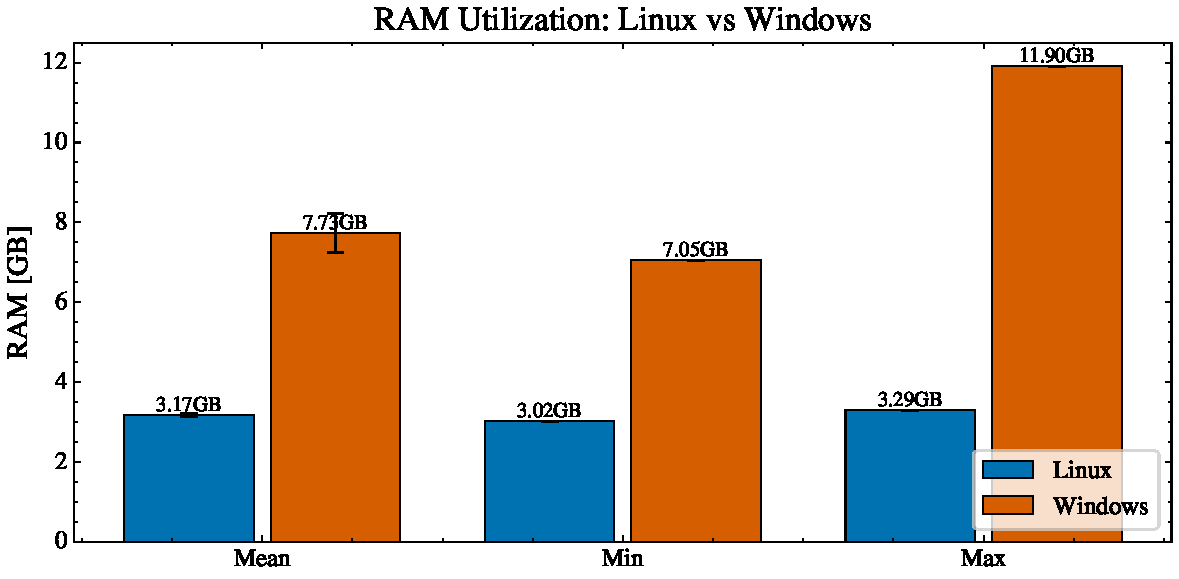
\includegraphics[width=\textwidth]{Messungen/OLD_10T/ram_bars_combined.pdf}
\caption{\acs{RAM}-Auslastung der Referenzmessung auf Linux und Windows bei zehn Threads, dargestellt als Balkendiagramm mit Mittelwerten und Standardabweichungen aus 20 Messläufen}
\label{fig:ref-10t-ram}
\end{figure}

\begin{figure}[H]
\centering
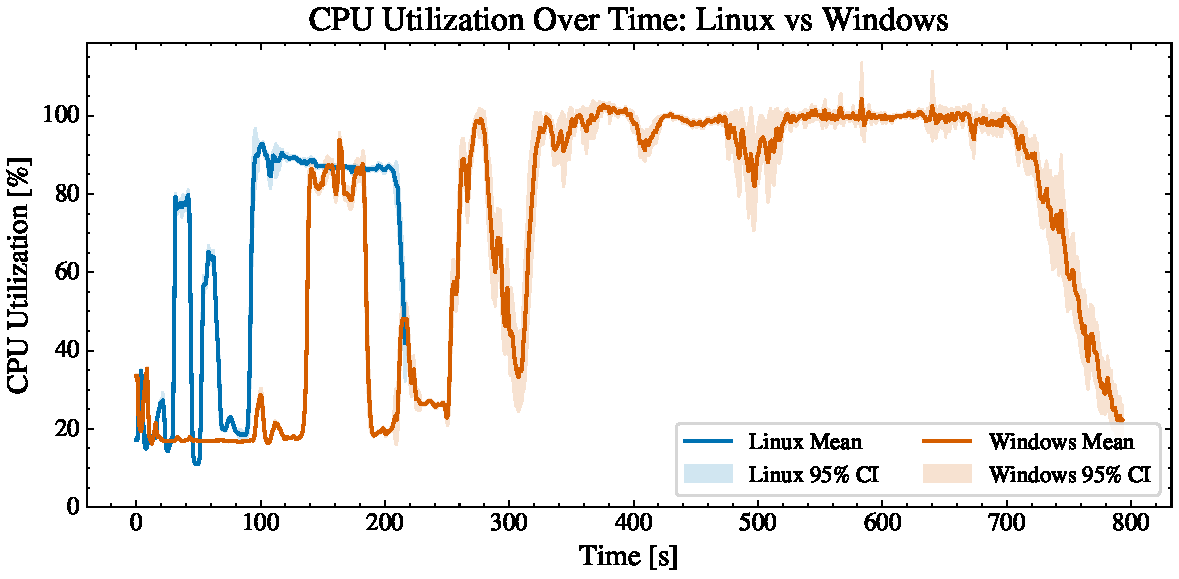
\includegraphics[width=\textwidth]{Messungen/OLD_10T/cpu_timeseries_combined.pdf}
\caption{Zeitlicher Verlauf der \acs{CPU}-Auslastung der Referenzmessung auf Linux und Windows bei zehn Threads}
\label{fig:ref-10t-cpu-ts}
\end{figure}

\begin{figure}[H]
\centering
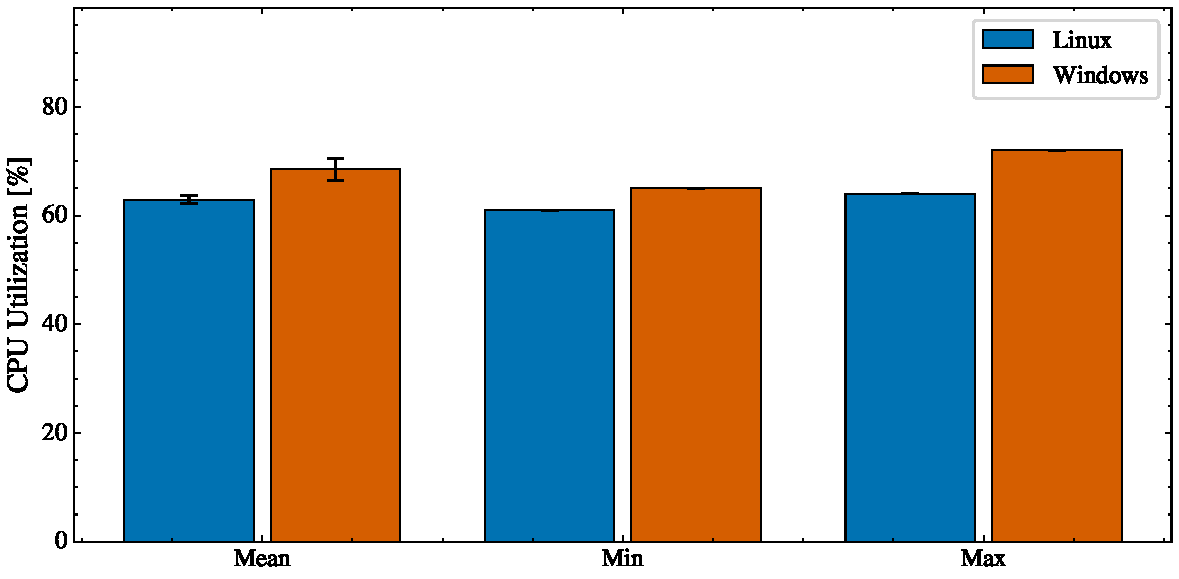
\includegraphics[width=\textwidth]{Messungen/OLD_10T/cpu_bars_combined.pdf}
\caption{\acs{CPU}-Auslastung der Referenzmessung auf Linux und Windows bei zehn Threads, dargestellt als Balkendiagramm mit Mittelwerten und Standardabweichungen aus 20 Messläufen}
\label{fig:ref-10t-cpu}
\end{figure}

\subsection{Vergleich}
\begin{figure}[H]
\centering
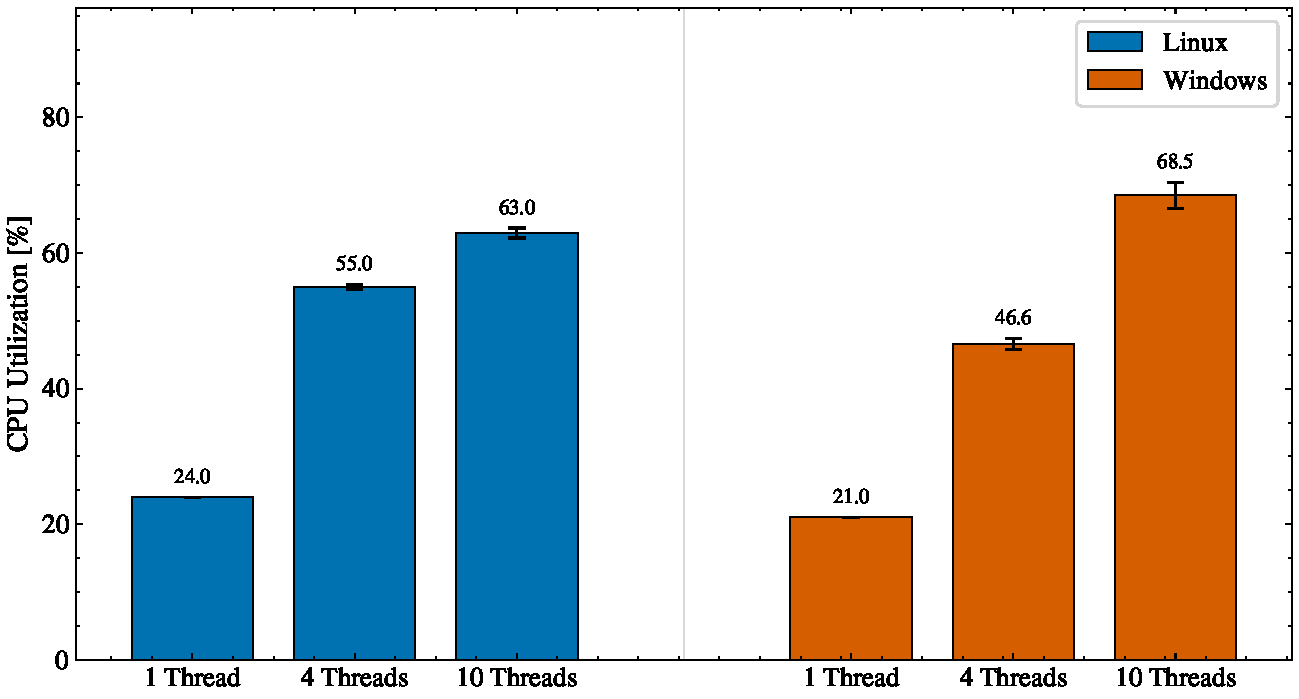
\includegraphics[width=\textwidth]{Messungen/Thread_Comparison/thread_referenz_cpu.pdf}
\caption{Vergleich der \acs{CPU}-Auslastung der Referenzmessung auf Linux und Windows über ein, vier und zehn Threads, dargestellt als Balkendiagramm mit Mittelwerten und Standardabweichungen aus 20 Messläufen}
\label{fig:ref-threadcmp-cpu}
\end{figure}

\begin{figure}[H]
\centering
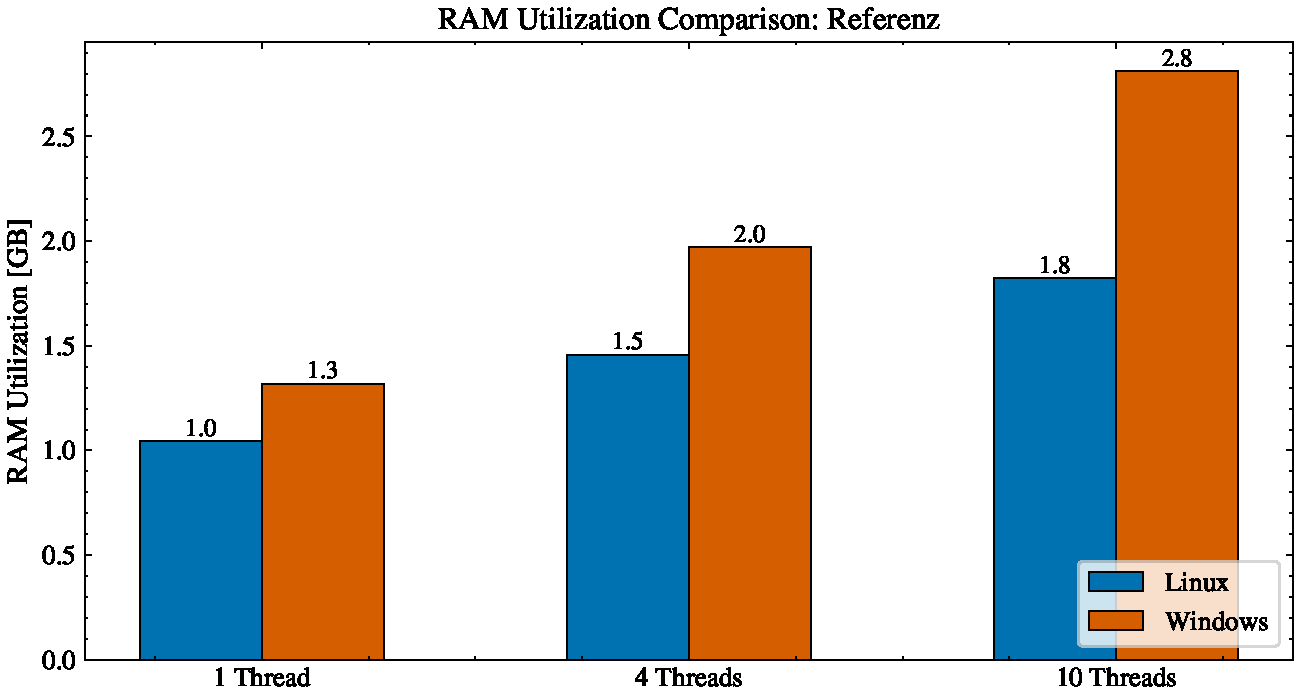
\includegraphics[width=\textwidth]{Messungen/Thread_Comparison/thread_referenz_ram.pdf}
\caption{Vergleich der \acs{RAM}-Auslastung der Referenzmessung auf Linux und Windows über ein, vier und zehn Threads, dargestellt als Balkendiagramm mit Mittelwerten und Standardabweichungen aus 20 Messläufen}
\label{fig:ref-threadcmp-ram}
\end{figure}

\begin{figure}[H]
\centering
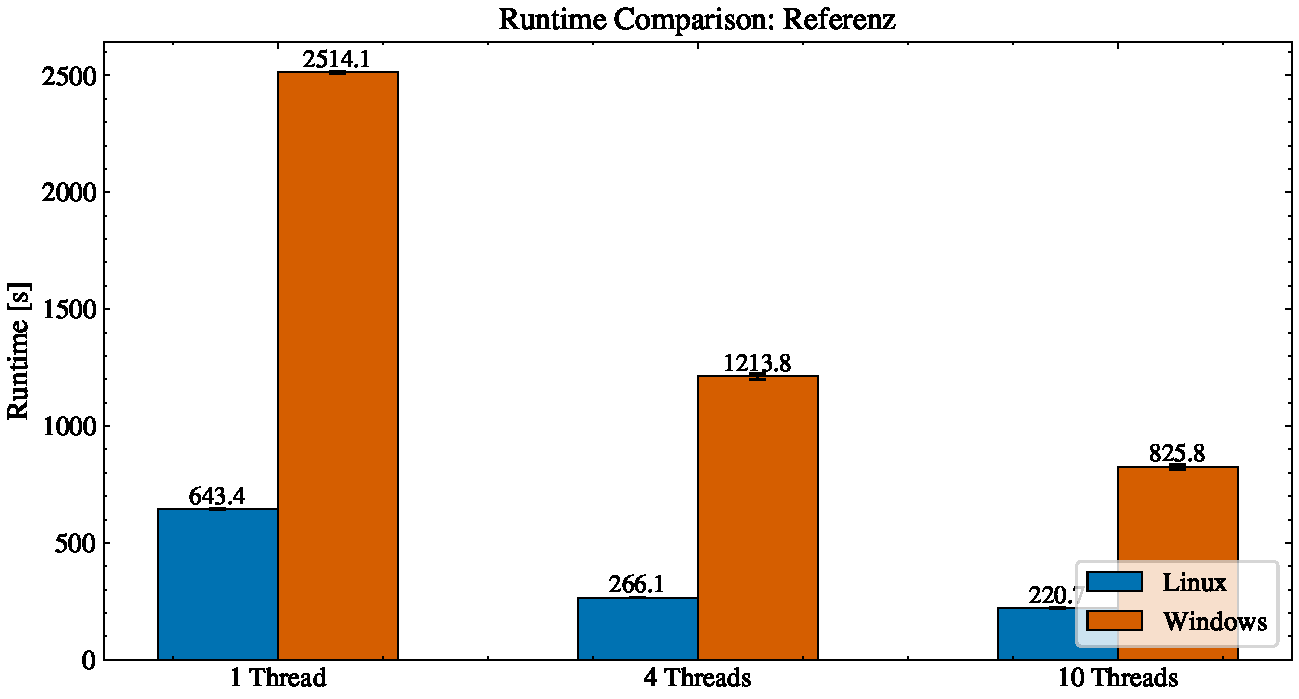
\includegraphics[width=\textwidth]{Messungen/Thread_Comparison/thread_referenz_runtime.pdf}
\caption{Vergleich der Laufzeiten der Referenzmessung auf Linux und Windows über ein, vier und zehn Threads, dargestellt als Balkendiagramm mit Mittelwerten und Standardabweichungen aus 20 Messläufen}
\label{fig:ref-threadcmp-runtime}
\end{figure}

\section{\acs{FIFO}\_50}

\subsection{Ein Thread}
\begin{figure}[H]
\centering
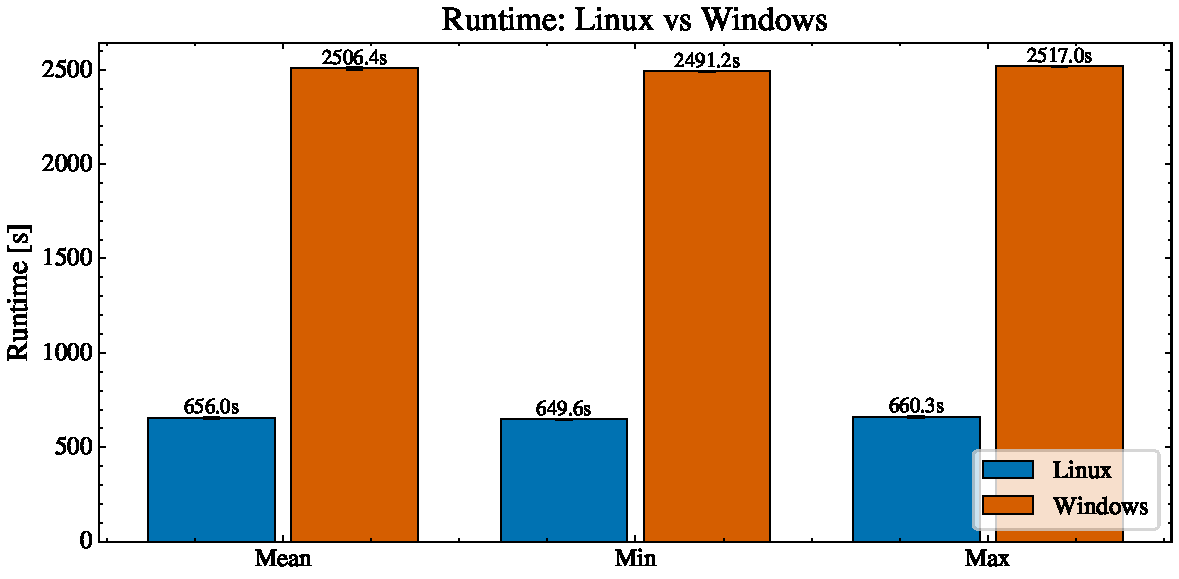
\includegraphics[width=\textwidth]{Messungen/FIFO_50_1T/runtime_bars_combined.pdf}
\caption{Laufzeiten des \acs{FIFO}\_50-Schedulers auf Linux und Windows bei einem Thread, dargestellt als Balkendiagramm mit Mittelwerten und Standardabweichungen aus 20 Messläufen}
\label{fig:fifo50-1t-runtime}
\end{figure}

\begin{figure}[H]
\centering
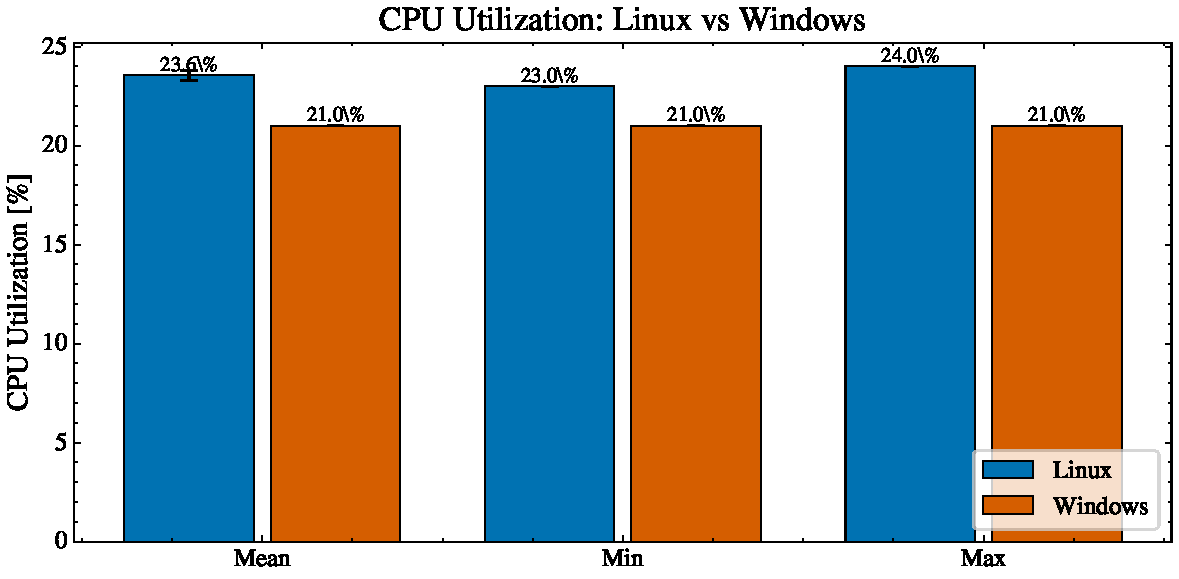
\includegraphics[width=\textwidth]{Messungen/FIFO_50_1T/cpu_bars_combined.pdf}
\caption{\acs{CPU}-Auslastung des \acs{FIFO}\_50-Schedulers auf Linux und Windows bei einem Thread, dargestellt als Balkendiagramm mit Mittelwerten und Standardabweichungen aus 20 Messläufen}
\label{fig:fifo50-1t-cpu}
\end{figure}

\begin{figure}[H]
\centering
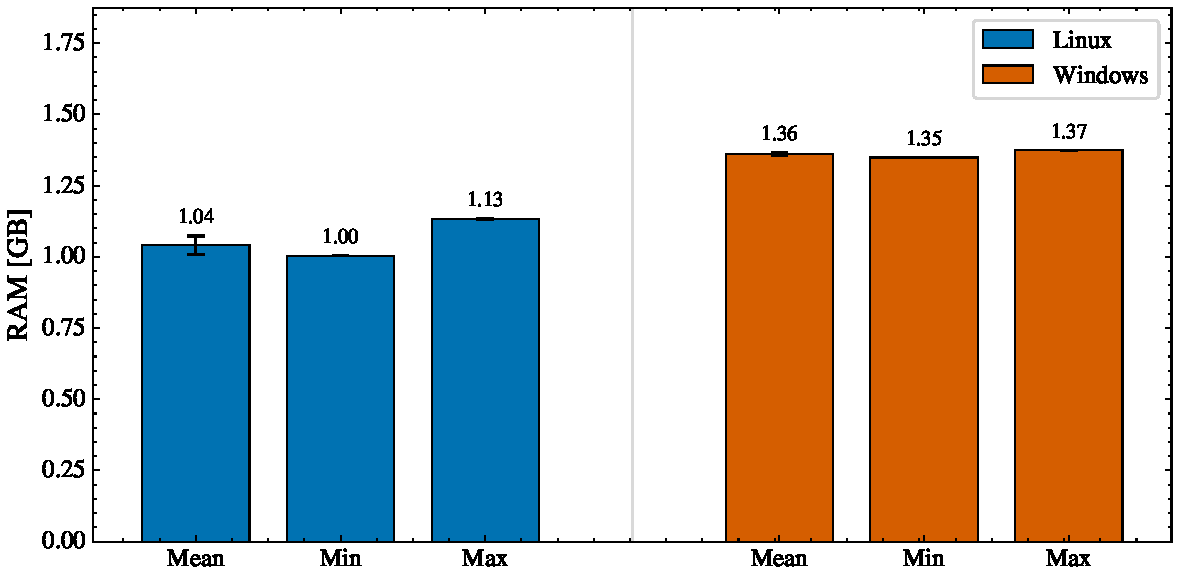
\includegraphics[width=\textwidth]{Messungen/FIFO_50_1T/ram_bars_combined.pdf}
\caption{\acs{RAM}-Auslastung des \acs{FIFO}\_50-Schedulers auf Linux und Windows bei einem Thread, dargestellt als Balkendiagramm mit Mittelwerten und Standardabweichungen aus 20 Messläufen}
\label{fig:fifo50-1t-ram}
\end{figure}

\begin{figure}[H]
\centering
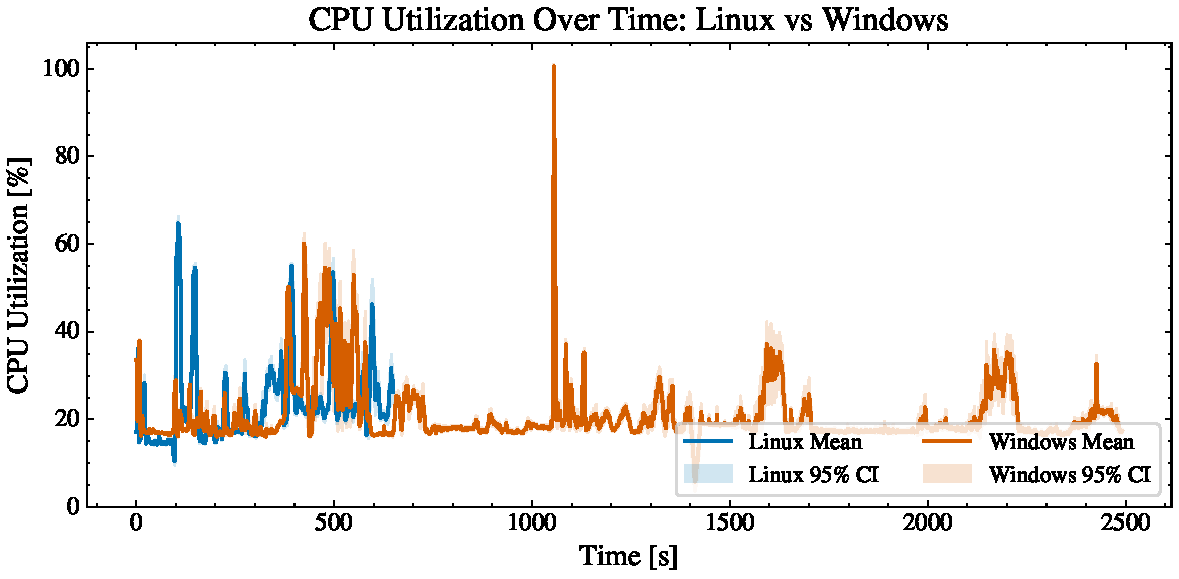
\includegraphics[width=\textwidth]{Messungen/FIFO_50_1T/cpu_timeseries_combined.pdf}
\caption{Zeitlicher Verlauf der \acs{CPU}-Auslastung des \acs{FIFO}\_50-Schedulers auf Linux und Windows bei einem Thread}
\label{fig:fifo50-1t-cpu-ts}
\end{figure}

\begin{figure}[H]
\centering
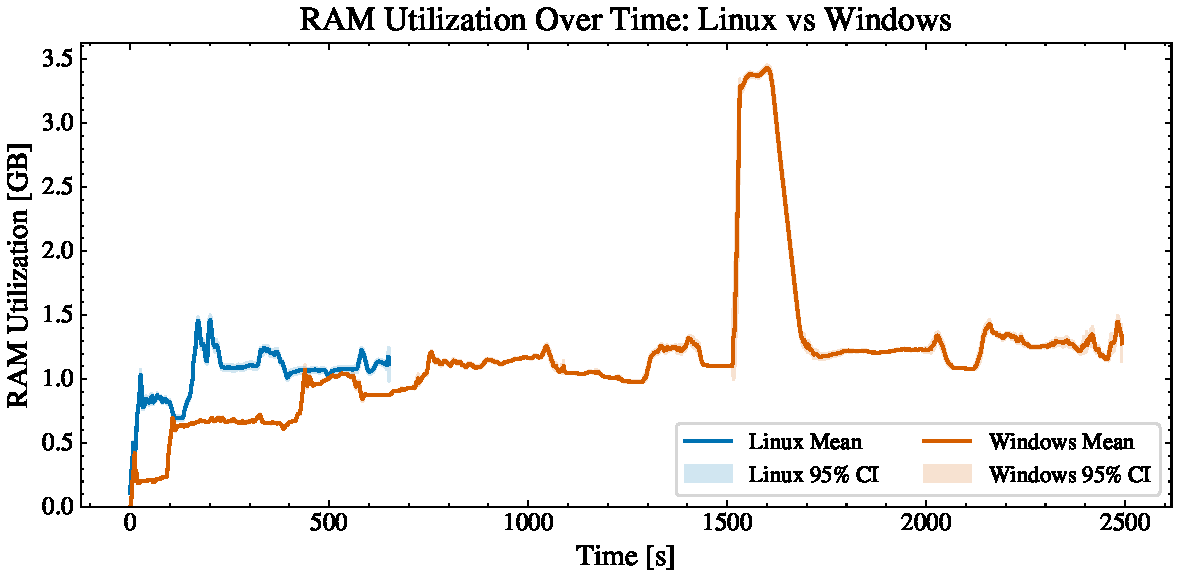
\includegraphics[width=\textwidth]{Messungen/FIFO_50_1T/ram_timeseries_combined.pdf}
\caption{Zeitlicher Verlauf der \acs{RAM}-Auslastung des \acs{FIFO}\_50-Schedulers auf Linux und Windows bei einem Thread}
\label{fig:fifo50-1t-ram-ts}
\end{figure}

\subsection{Vier Threads}
\begin{figure}[H]
\centering
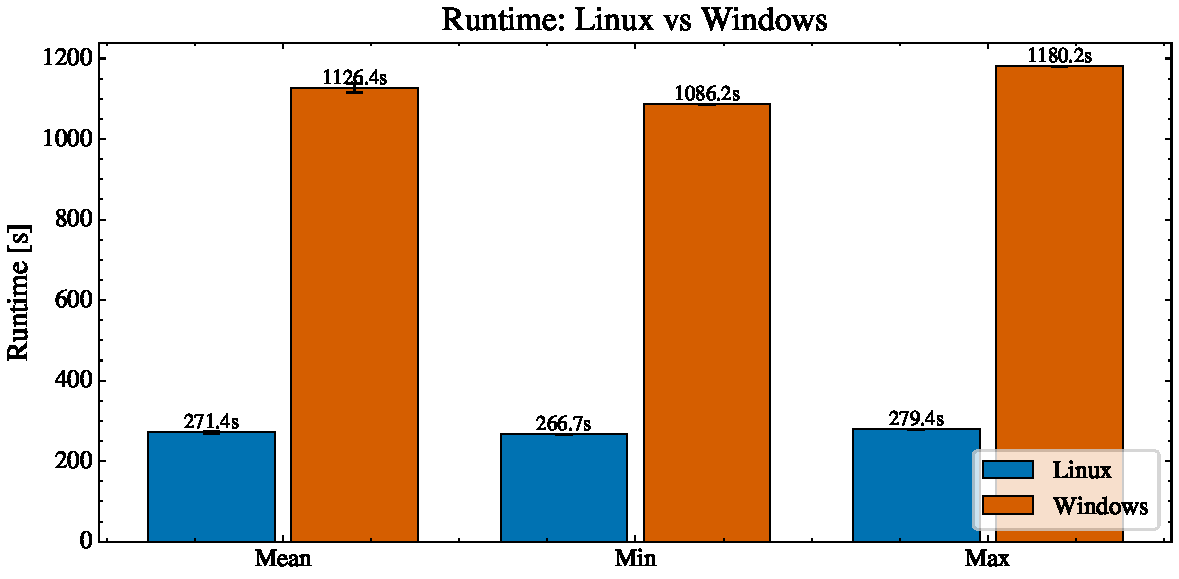
\includegraphics[width=\textwidth]{Messungen/FIFO_50_4T/runtime_bars_combined.pdf}
\caption{Laufzeiten des \acs{FIFO}\_50-Schedulers auf Linux und Windows bei vier Threads, dargestellt als Balkendiagramm mit Mittelwerten und Standardabweichungen aus 20 Messläufen}
\label{fig:fifo50-4t-runtime}
\end{figure}

\begin{figure}[H]
\centering
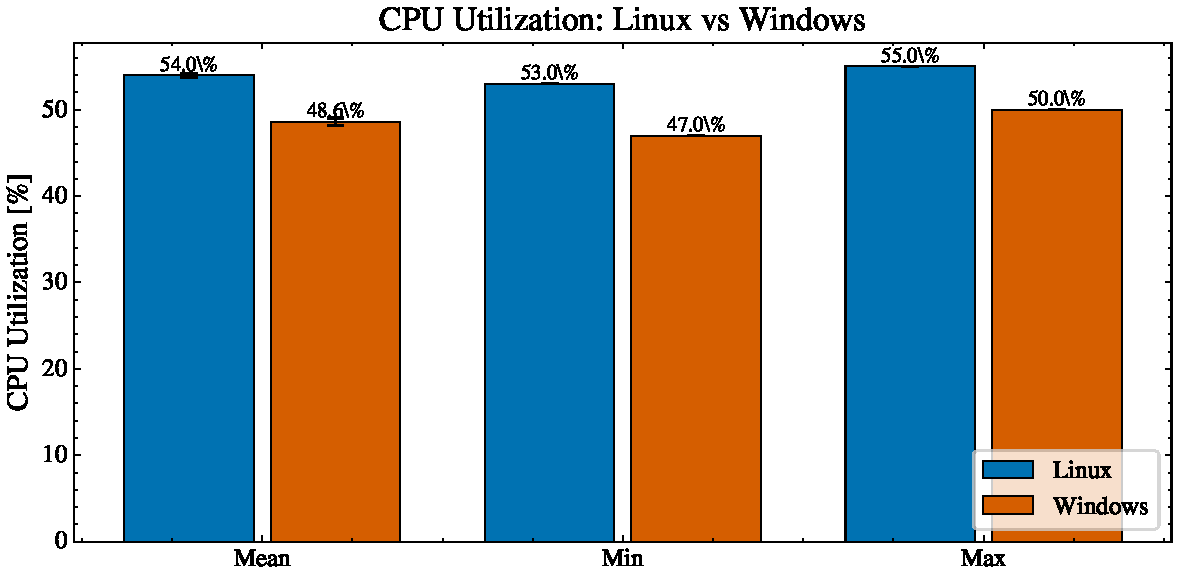
\includegraphics[width=\textwidth]{Messungen/FIFO_50_4T/cpu_bars_combined.pdf}
\caption{\acs{CPU}-Auslastung des \acs{FIFO}\_50-Schedulers auf Linux und Windows bei vier Threads, dargestellt als Balkendiagramm mit Mittelwerten und Standardabweichungen aus 20 Messläufen}
\label{fig:fifo50-4t-cpu}
\end{figure}

\begin{figure}[H]
\centering
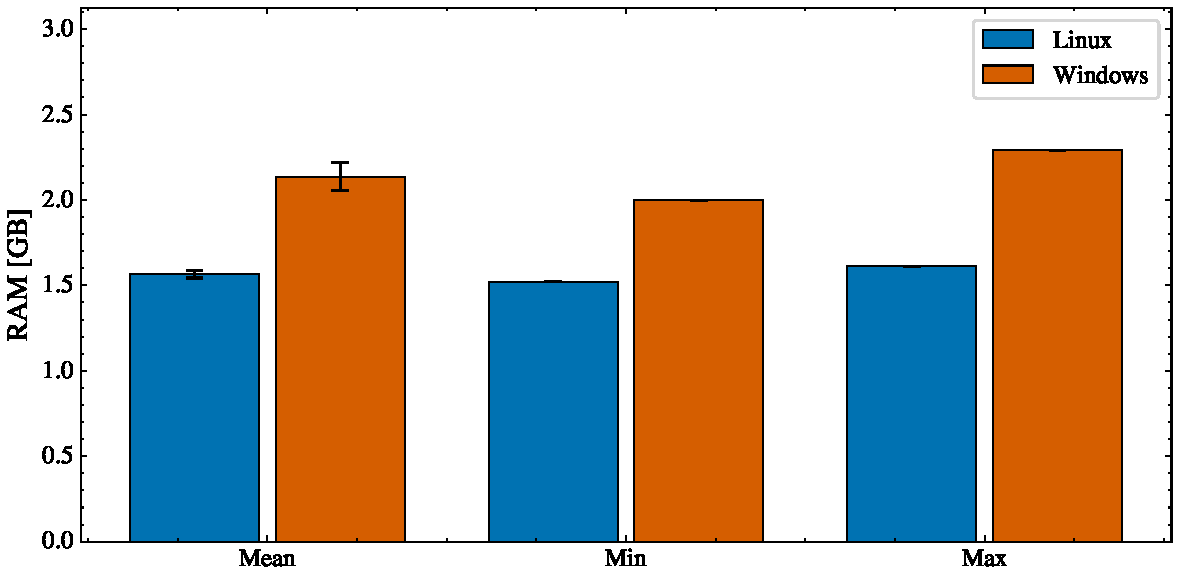
\includegraphics[width=\textwidth]{Messungen/FIFO_50_4T/ram_bars_combined.pdf}
\caption{\acs{RAM}-Auslastung des \acs{FIFO}\_50-Schedulers auf Linux und Windows bei vier Threads, dargestellt als Balkendiagramm mit Mittelwerten und Standardabweichungen aus 20 Messläufen}
\label{fig:fifo50-4t-ram}
\end{figure}

\begin{figure}[H]
\centering
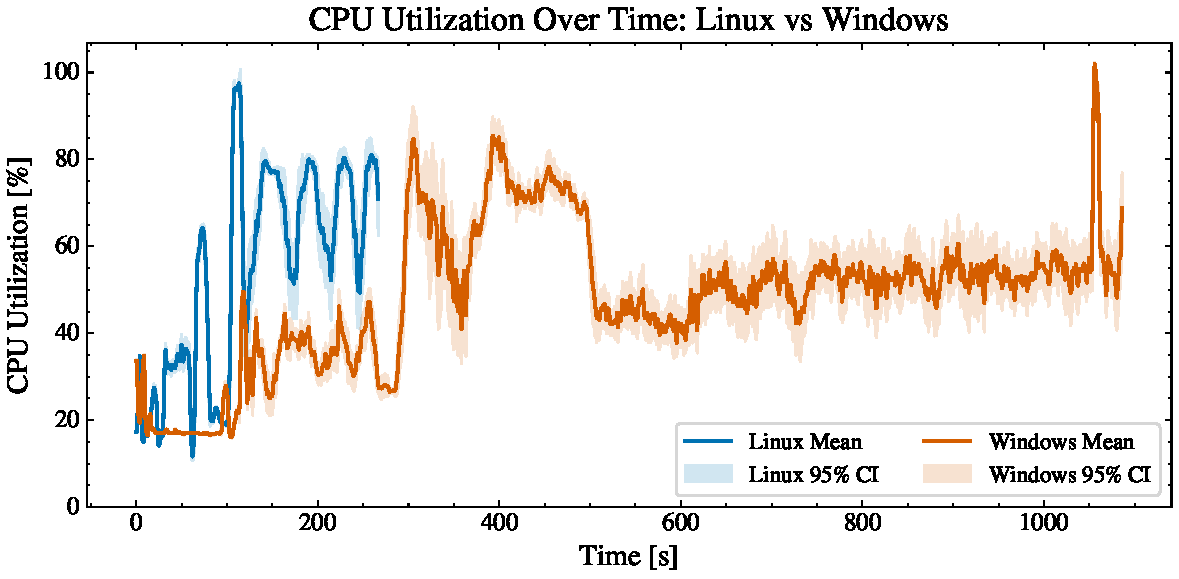
\includegraphics[width=\textwidth]{Messungen/FIFO_50_4T/cpu_timeseries_combined.pdf}
\caption{Zeitlicher Verlauf der \acs{CPU}-Auslastung des \acs{FIFO}\_50-Schedulers auf Linux und Windows bei vier Threads}
\label{fig:fifo50-4t-cpu-ts}
\end{figure}

\begin{figure}[H]
\centering
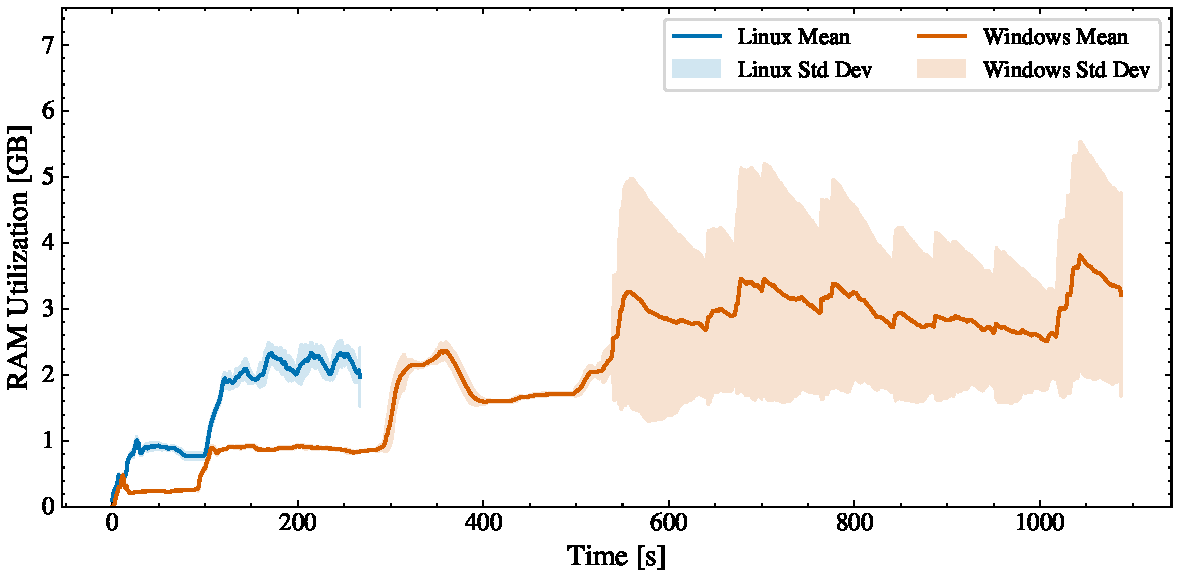
\includegraphics[width=\textwidth]{Messungen/FIFO_50_4T/ram_timeseries_combined.pdf}
\caption{Zeitlicher Verlauf der \acs{RAM}-Auslastung des \acs{FIFO}\_50-Schedulers auf Linux und Windows bei vier Threads}
\label{fig:fifo50-4t-ram-ts}
\end{figure}

\subsection{Zehn Threads}
\begin{figure}[H]
\centering
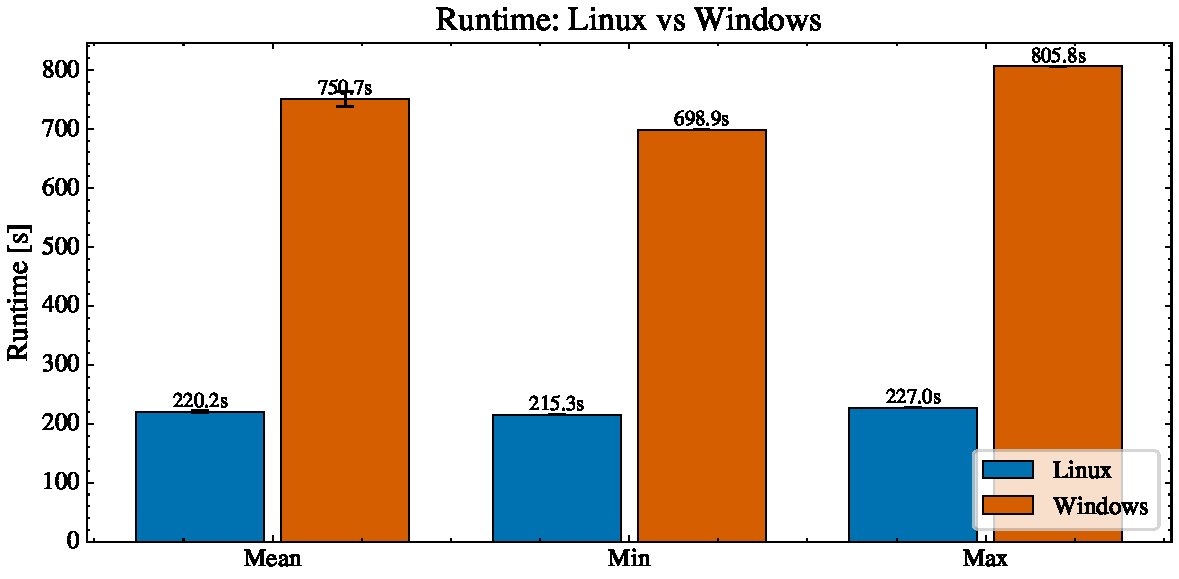
\includegraphics[width=\textwidth]{Messungen/FIFO_50_10T/runtime_bars_combined.pdf}
\caption{Laufzeiten des \acs{FIFO}\_50-Schedulers auf Linux und Windows bei zehn Threads, dargestellt als Balkendiagramm mit Mittelwerten und Standardabweichungen aus 20 Messläufen}
\label{fig:fifo50-10t-runtime}
\end{figure}

\begin{figure}[H]
\centering
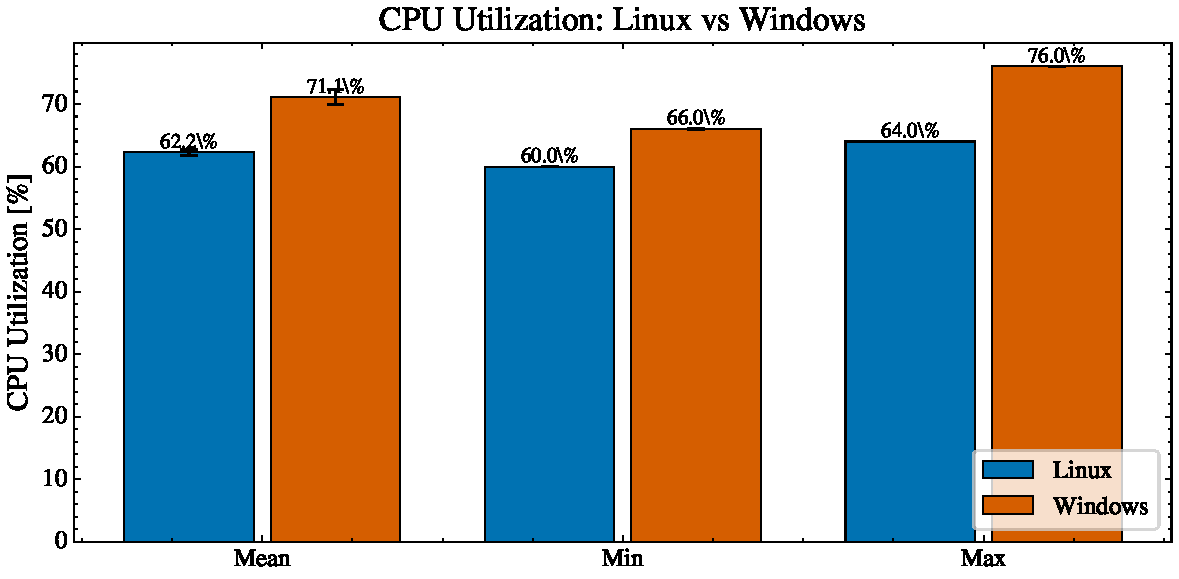
\includegraphics[width=\textwidth]{Messungen/FIFO_50_10T/cpu_bars_combined.pdf}
\caption{\acs{CPU}-Auslastung des \acs{FIFO}\_50-Schedulers auf Linux und Windows bei zehn Threads, dargestellt als Balkendiagramm mit Mittelwerten und Standardabweichungen aus 20 Messläufen}
\label{fig:fifo50-10t-cpu}
\end{figure}

\begin{figure}[H]
\centering
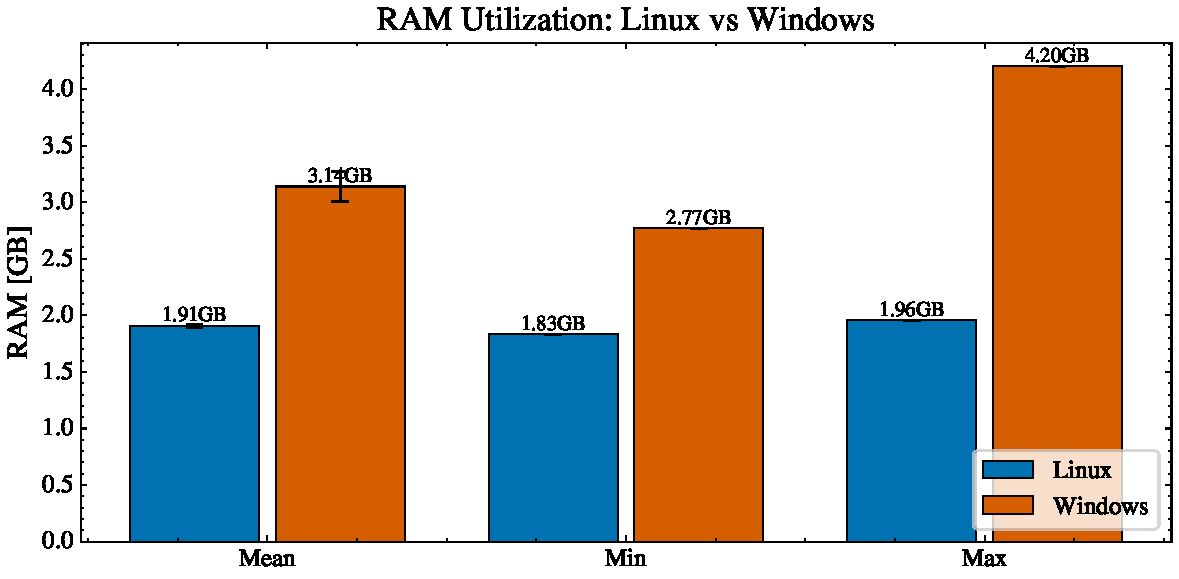
\includegraphics[width=\textwidth]{Messungen/FIFO_50_10T/ram_bars_combined.pdf}
\caption{\acs{RAM}-Auslastung des \acs{FIFO}\_50-Schedulers auf Linux und Windows bei zehn Threads, dargestellt als Balkendiagramm mit Mittelwerten und Standardabweichungen aus 20 Messläufen}
\label{fig:fifo50-10t-ram}
\end{figure}

\begin{figure}[H]
\centering
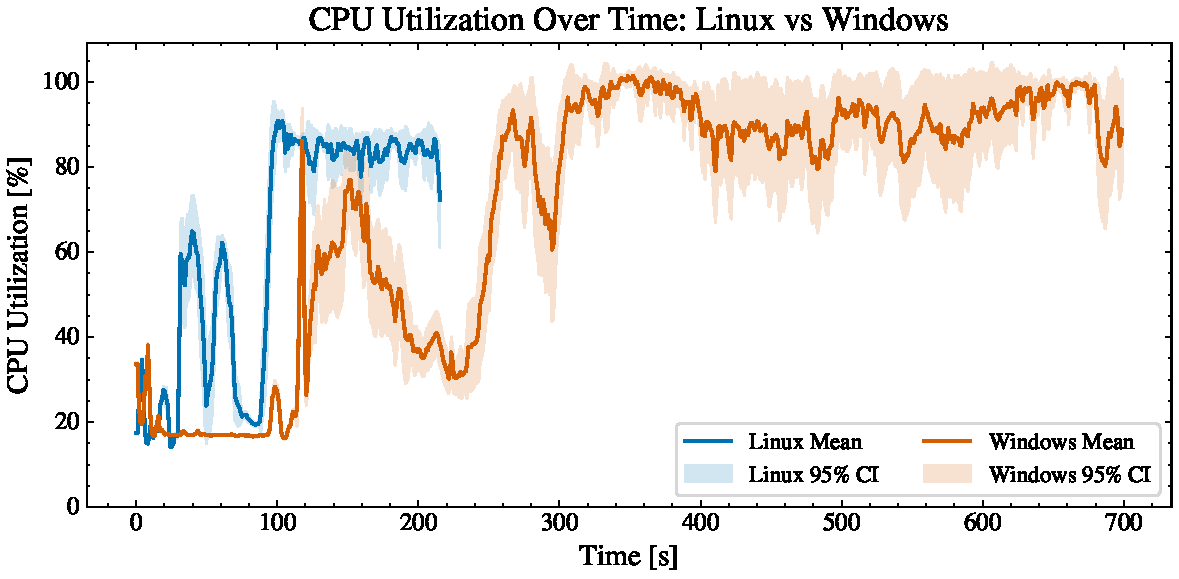
\includegraphics[width=\textwidth]{Messungen/FIFO_50_10T/cpu_timeseries_combined.pdf}
\caption{Zeitlicher Verlauf der \acs{CPU}-Auslastung des \acs{FIFO}\_50-Schedulers auf Linux und Windows bei zehn Threads}
\label{fig:fifo50-10t-cpu-ts}
\end{figure}

\begin{figure}[H]
\centering
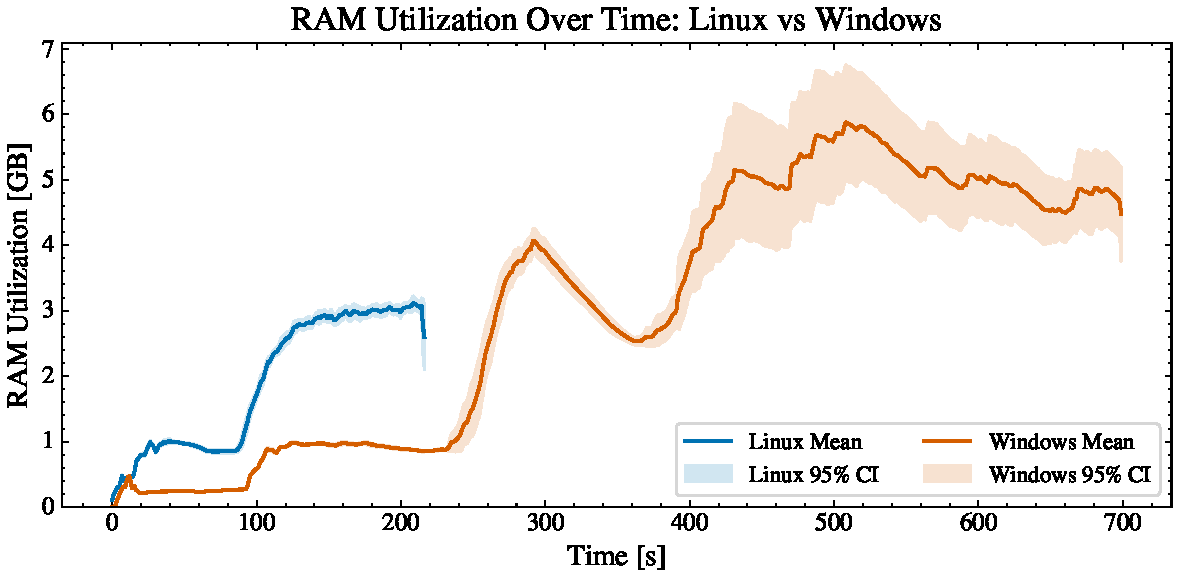
\includegraphics[width=\textwidth]{Messungen/FIFO_50_10T/ram_timeseries_combined.pdf}
\caption{Zeitlicher Verlauf der \acs{RAM}-Auslastung des \acs{FIFO}\_50-Schedulers auf Linux und Windows bei zehn Threads}
\label{fig:fifo50-10t-ram-ts}
\end{figure}

\subsection{Vergleich}
\begin{figure}[H]
\centering
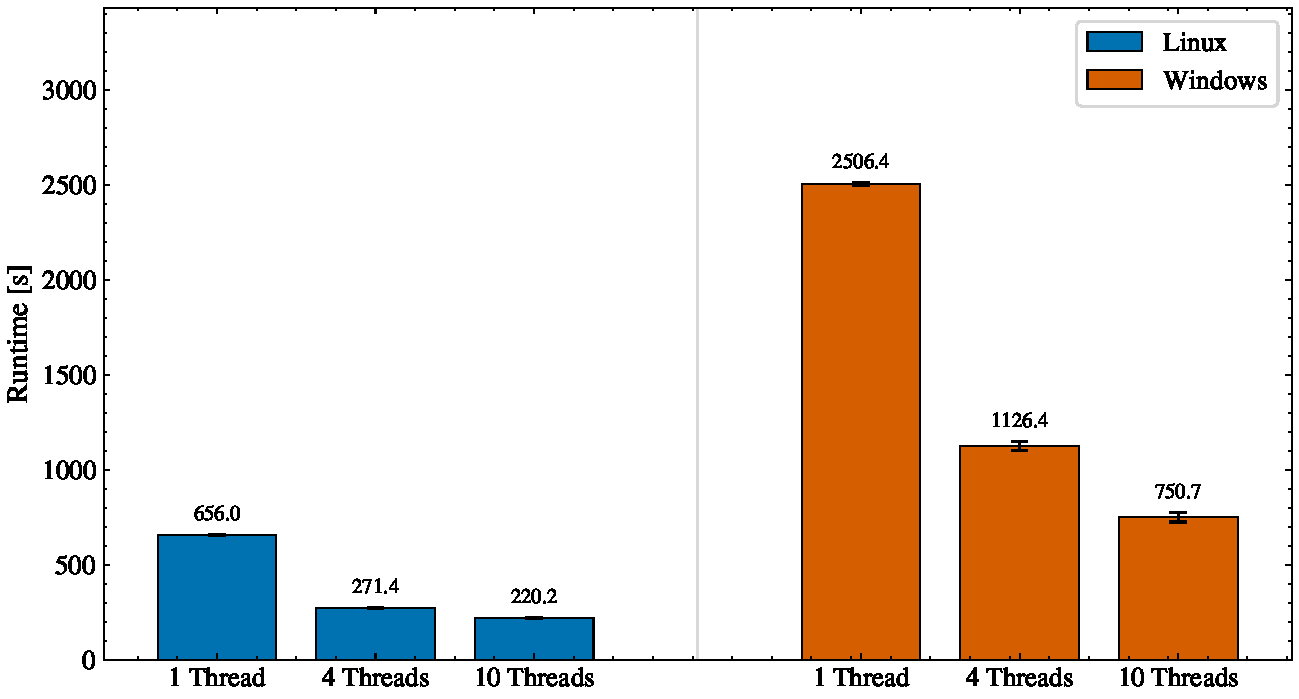
\includegraphics[width=\textwidth]{Messungen/Thread_Comparison/thread_fifo_50_runtime.pdf}
\caption{Vergleich der Laufzeiten des \acs{FIFO}\_50-Schedulers auf Linux und Windows über ein, vier und zehn Threads, dargestellt als Balkendiagramm mit Mittelwerten und Standardabweichungen aus 20 Messläufen}
\label{fig:fifo50-threadcmp-runtime}
\end{figure}

\begin{figure}[H]
\centering
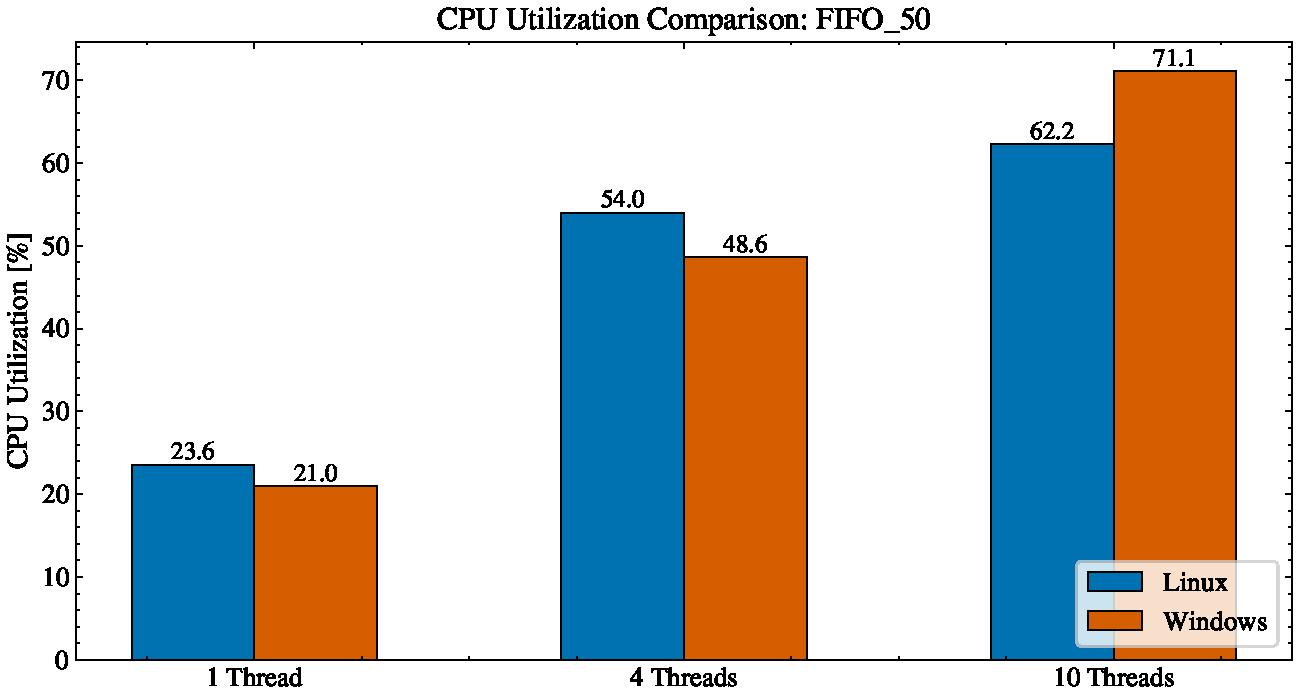
\includegraphics[width=\textwidth]{Messungen/Thread_Comparison/thread_fifo_50_cpu.pdf}
\caption{Vergleich der \acs{CPU}-Auslastung des \acs{FIFO}\_50-Schedulers auf Linux und Windows über ein, vier und zehn Threads, dargestellt als Balkendiagramm mit Mittelwerten und Standardabweichungen aus 20 Messläufen}
\label{fig:fifo50-threadcmp-cpu}
\end{figure}

\begin{figure}[H]
\centering
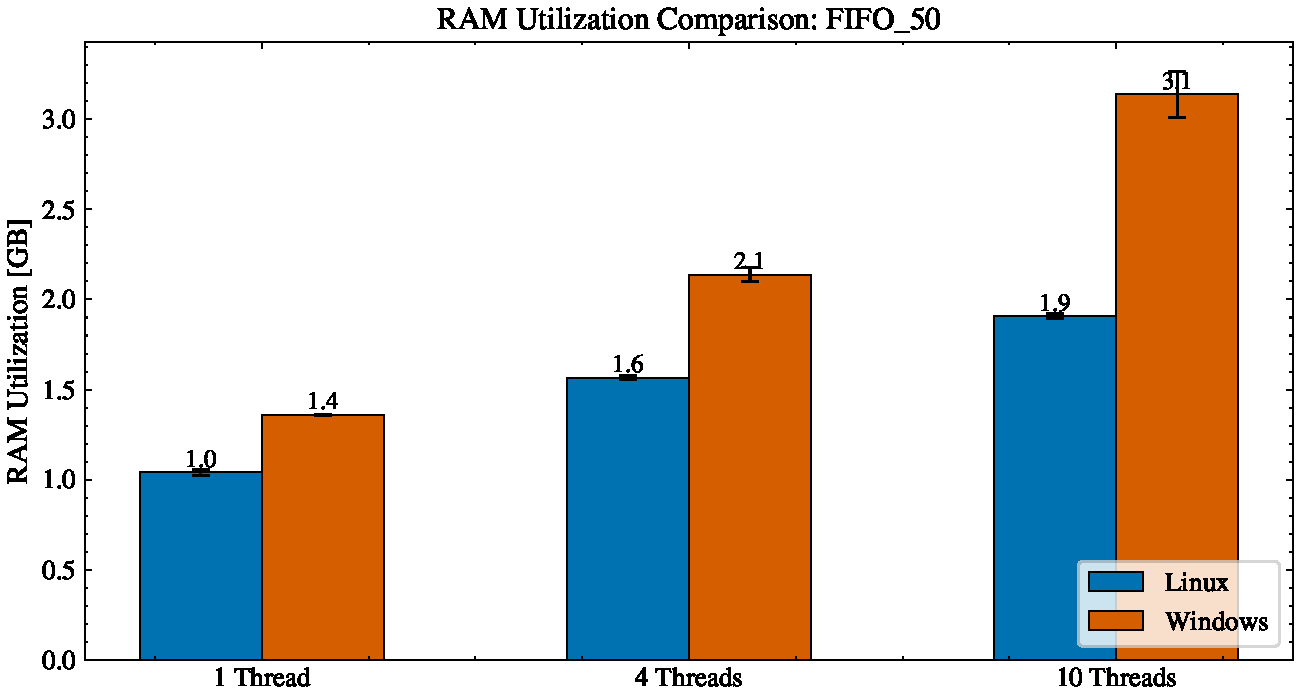
\includegraphics[width=\textwidth]{Messungen/Thread_Comparison/thread_fifo_50_ram.pdf}
\caption{Vergleich der \acs{RAM}-Auslastung des \acs{FIFO}\_50-Schedulers auf Linux und Windows über ein, vier und zehn Threads, dargestellt als Balkendiagramm mit Mittelwerten und Standardabweichungen aus 20 Messläufen}
\label{fig:fifo50-threadcmp-ram}
\end{figure}


\section{\acs{FIFO}\_500}

\subsection{Ein Thread}
\begin{figure}[H]
\centering
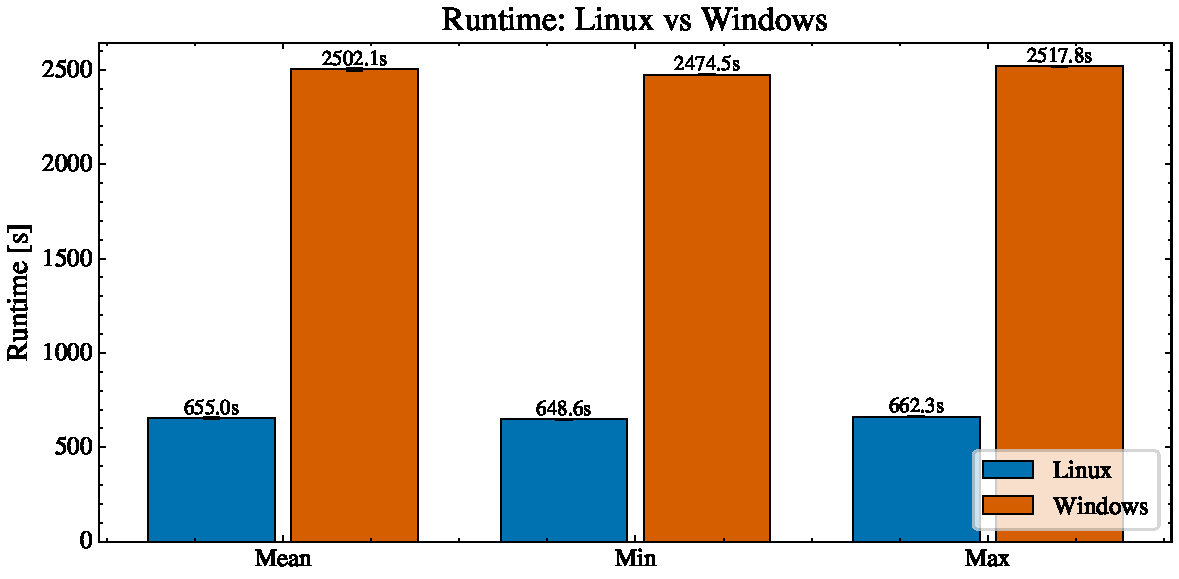
\includegraphics[width=\textwidth]{Messungen/FIFO_500_1T/runtime_bars_combined.pdf}
\caption{Laufzeiten des \acs{FIFO}\_500-Schedulers auf Linux und Windows bei einem Thread, dargestellt als Balkendiagramm mit Mittelwerten und Standardabweichungen aus 20 Messläufen}
\label{fig:fifo500-1t-runtime}
\end{figure}

\begin{figure}[H]
\centering
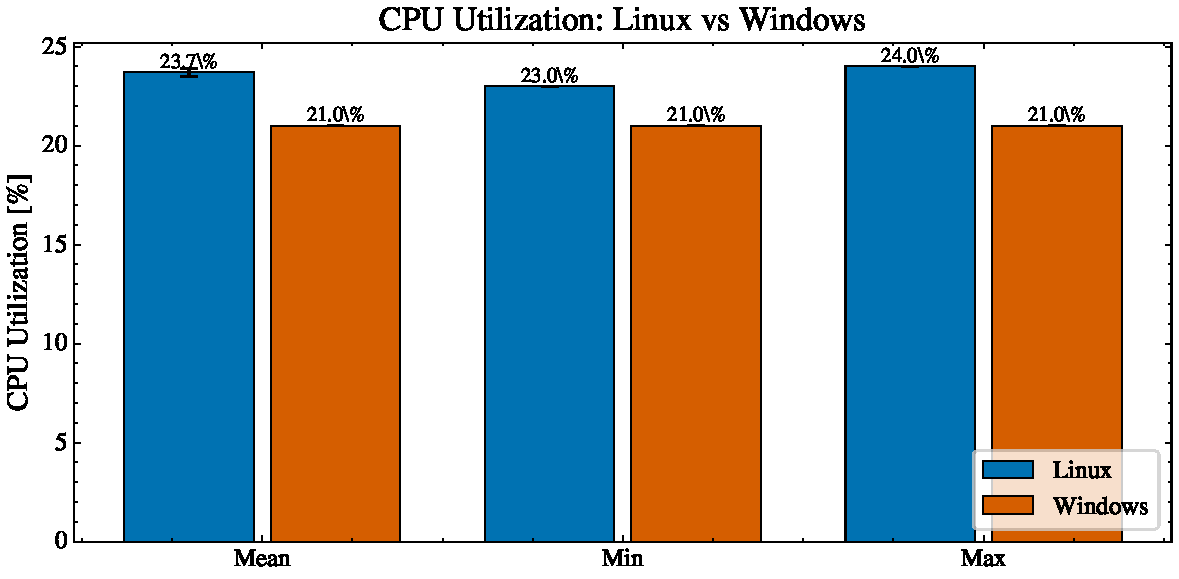
\includegraphics[width=\textwidth]{Messungen/FIFO_500_1T/cpu_bars_combined.pdf}
\caption{\acs{CPU}-Auslastung des \acs{FIFO}\_500-Schedulers auf Linux und Windows bei einem Thread, dargestellt als Balkendiagramm mit Mittelwerten und Standardabweichungen aus 20 Messläufen}
\label{fig:fifo500-1t-cpu}
\end{figure}

\begin{figure}[H]
\centering
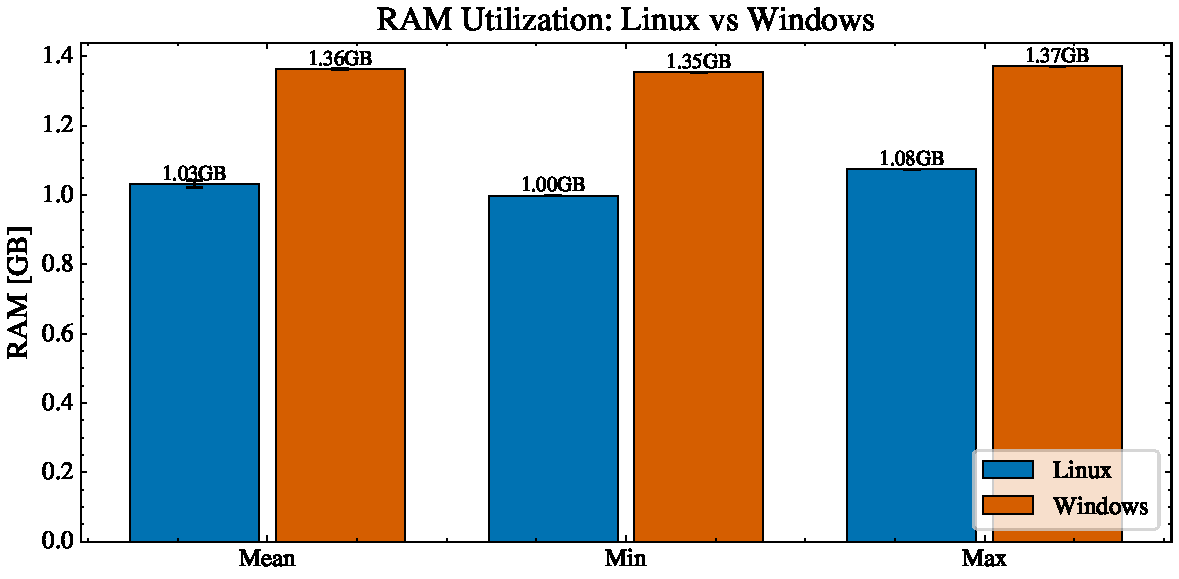
\includegraphics[width=\textwidth]{Messungen/FIFO_500_1T/ram_bars_combined.pdf}
\caption{\acs{RAM}-Auslastung des \acs{FIFO}\_500-Schedulers auf Linux und Windows bei einem Thread, dargestellt als Balkendiagramm mit Mittelwerten und Standardabweichungen aus 20 Messläufen}
\label{fig:fifo500-1t-ram}
\end{figure}

\begin{figure}[H]
\centering
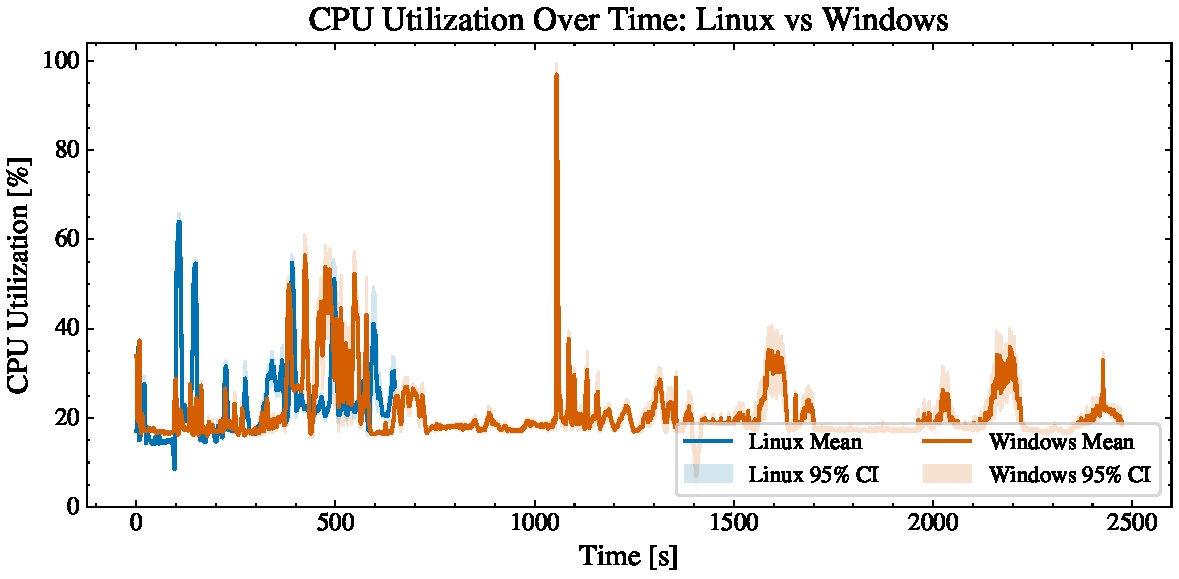
\includegraphics[width=\textwidth]{Messungen/FIFO_500_1T/cpu_timeseries_combined.pdf}
\caption{Zeitlicher Verlauf der \acs{CPU}-Auslastung des \acs{FIFO}\_500-Schedulers auf Linux und Windows bei einem Thread}
\label{fig:fifo500-1t-cpu-ts}
\end{figure}

\begin{figure}[H]
\centering
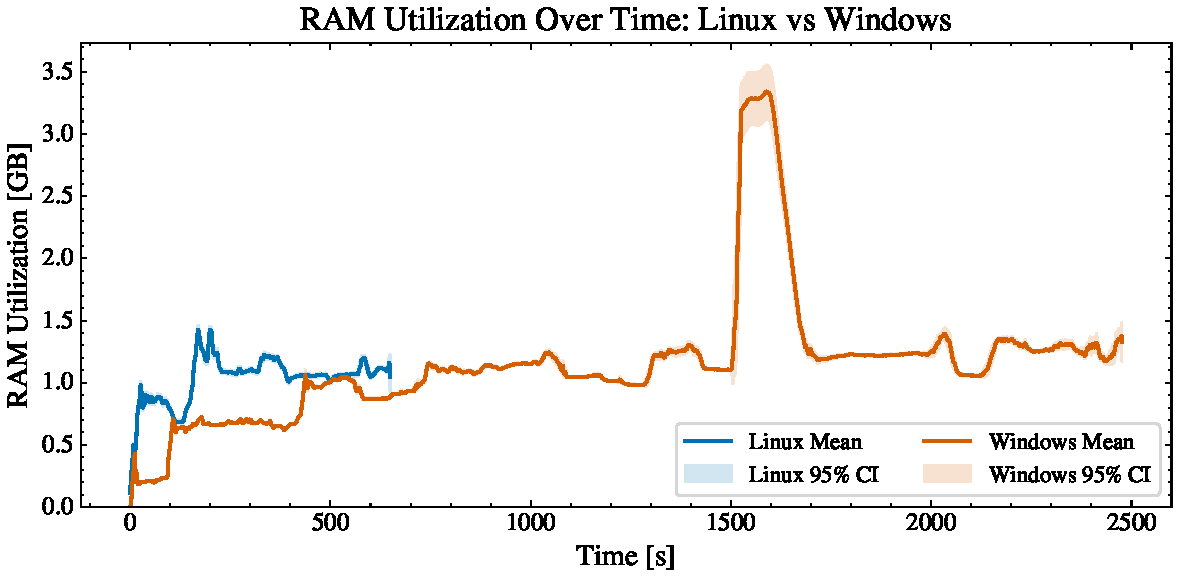
\includegraphics[width=\textwidth]{Messungen/FIFO_500_1T/ram_timeseries_combined.pdf}
\caption{Zeitlicher Verlauf der \acs{RAM}-Auslastung des \acs{FIFO}\_500-Schedulers auf Linux und Windows bei einem Thread}
\label{fig:fifo500-1t-ram-ts}
\end{figure}

\subsection{Vier Threads}
\begin{figure}[H]
\centering
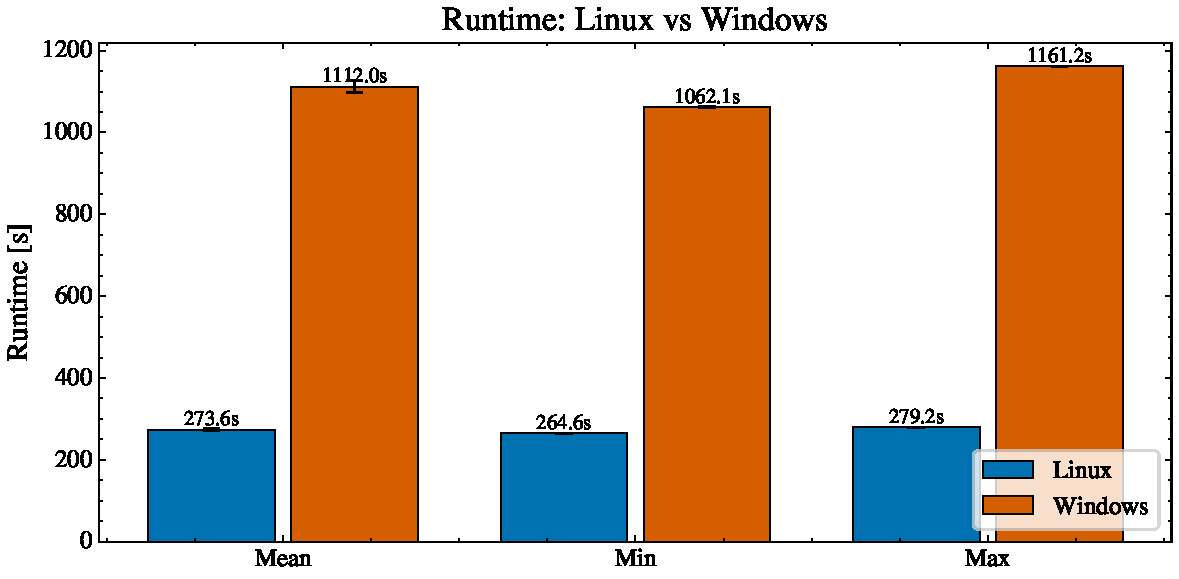
\includegraphics[width=\textwidth]{Messungen/FIFO_500_4T/runtime_bars_combined.pdf}
\caption{Laufzeiten des \acs{FIFO}\_500-Schedulers auf Linux und Windows bei vier Threads, dargestellt als Balkendiagramm mit Mittelwerten und Standardabweichungen aus 20 Messläufen}
\label{fig:fifo500-4t-runtime}
\end{figure}

\begin{figure}[H]
\centering
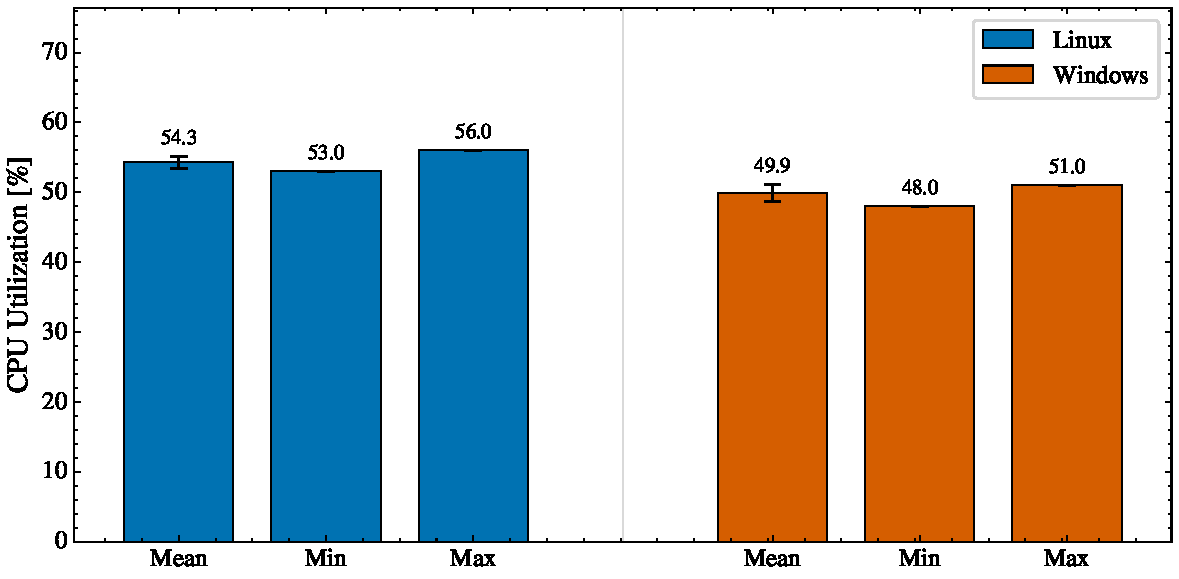
\includegraphics[width=\textwidth]{Messungen/FIFO_500_4T/cpu_bars_combined.pdf}
\caption{\acs{CPU}-Auslastung des \acs{FIFO}\_500-Schedulers auf Linux und Windows bei vier Threads, dargestellt als Balkendiagramm mit Mittelwerten und Standardabweichungen aus 20 Messläufen}
\label{fig:fifo500-4t-cpu}
\end{figure}

\begin{figure}[H]
\centering
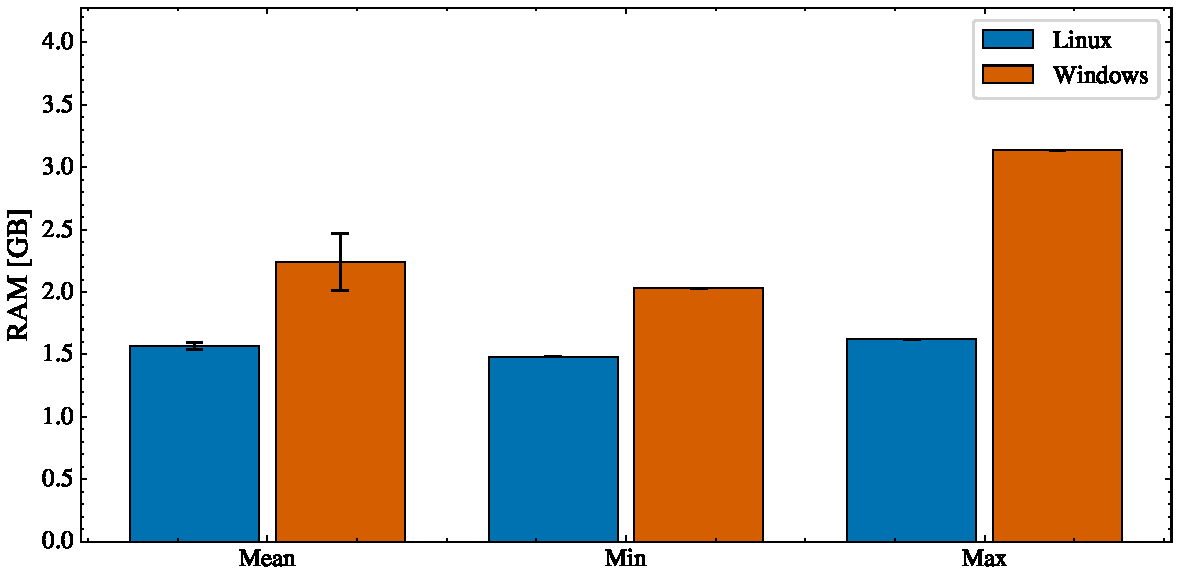
\includegraphics[width=\textwidth]{Messungen/FIFO_500_4T/ram_bars_combined.pdf}
\caption{\acs{RAM}-Auslastung des \acs{FIFO}\_500-Schedulers auf Linux und Windows bei vier Threads, dargestellt als Balkendiagramm mit Mittelwerten und Standardabweichungen aus 20 Messläufen}
\label{fig:fifo500-4t-ram}
\end{figure}

\begin{figure}[H]
\centering
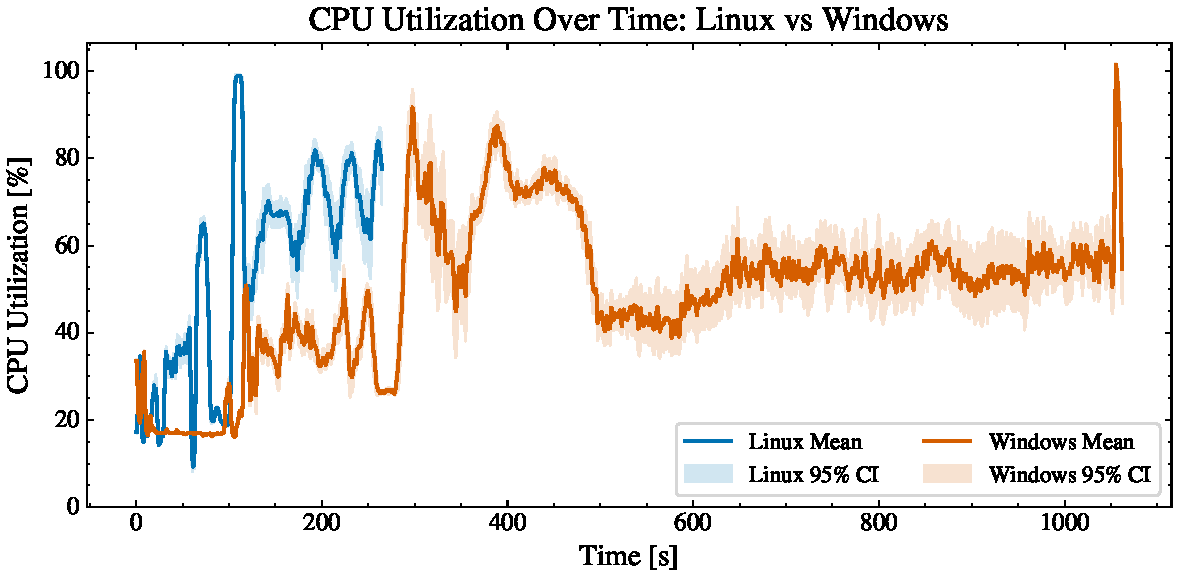
\includegraphics[width=\textwidth]{Messungen/FIFO_500_4T/cpu_timeseries_combined.pdf}
\caption{Zeitlicher Verlauf der \acs{CPU}-Auslastung des \acs{FIFO}\_500-Schedulers auf Linux und Windows bei vier Threads}
\label{fig:fifo500-4t-cpu-ts}
\end{figure}

\begin{figure}[H]
\centering
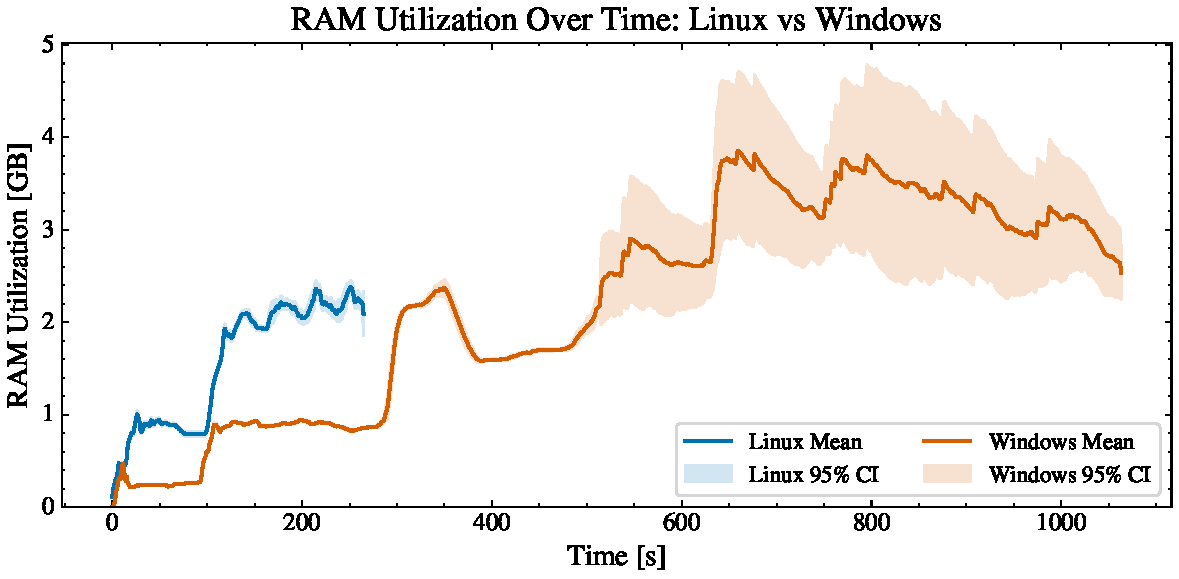
\includegraphics[width=\textwidth]{Messungen/FIFO_500_4T/ram_timeseries_combined.pdf}
\caption{Zeitlicher Verlauf der \acs{RAM}-Auslastung des \acs{FIFO}\_500-Schedulers auf Linux und Windows bei vier Threads}
\label{fig:fifo500-4t-ram-ts}
\end{figure}

\subsection{Zehn Threads}
\begin{figure}[H]
\centering
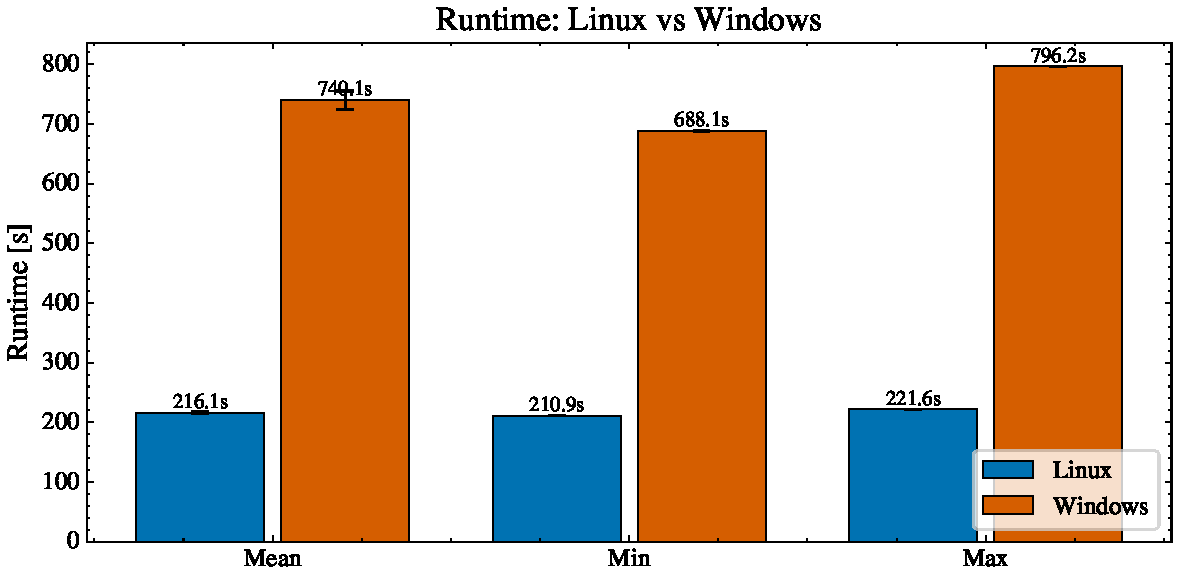
\includegraphics[width=\textwidth]{Messungen/FIFO_500_10T/runtime_bars_combined.pdf}
\caption{Laufzeiten des \acs{FIFO}\_500-Schedulers auf Linux und Windows bei zehn Threads, dargestellt als Balkendiagramm mit Mittelwerten und Standardabweichungen aus 20 Messläufen}
\label{fig:fifo500-10t-runtime}
\end{figure}

\begin{figure}[H]
\centering
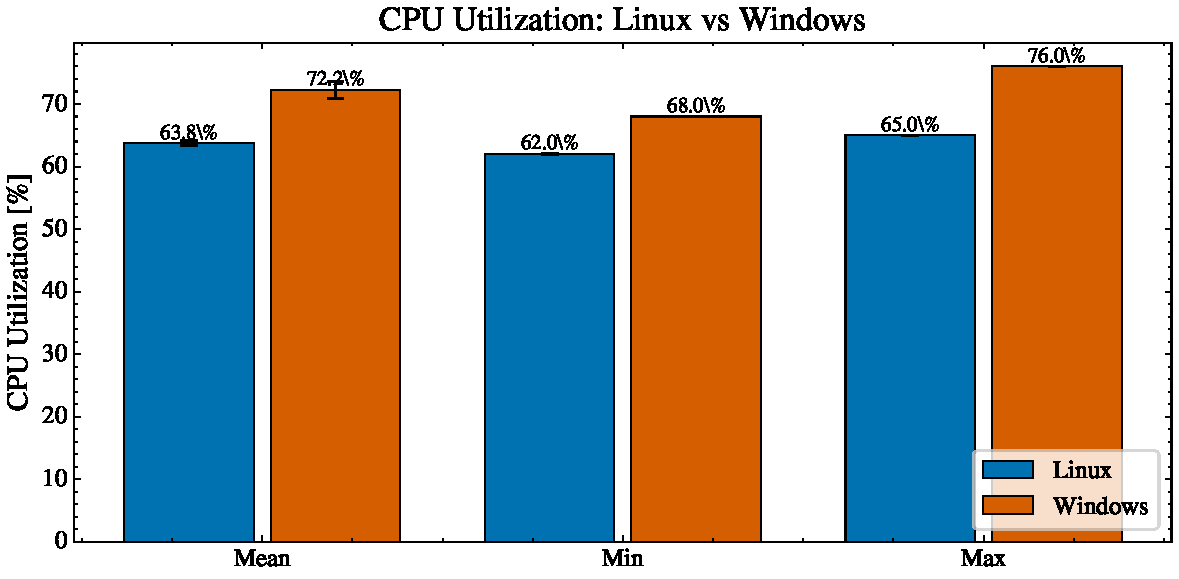
\includegraphics[width=\textwidth]{Messungen/FIFO_500_10T/cpu_bars_combined.pdf}
\caption{\acs{CPU}-Auslastung des \acs{FIFO}\_500-Schedulers auf Linux und Windows bei zehn Threads, dargestellt als Balkendiagramm mit Mittelwerten und Standardabweichungen aus 20 Messläufen}
\label{fig:fifo500-10t-cpu}
\end{figure}

\begin{figure}[H]
\centering
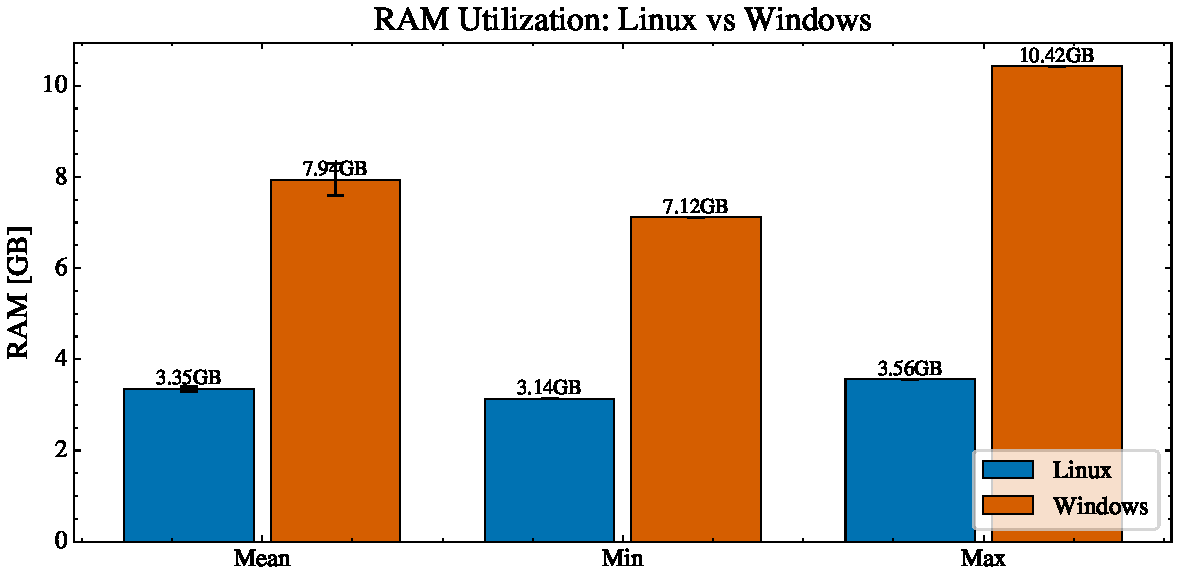
\includegraphics[width=\textwidth]{Messungen/FIFO_500_10T/ram_bars_combined.pdf}
\caption{\acs{RAM}-Auslastung des \acs{FIFO}\_500-Schedulers auf Linux und Windows bei zehn Threads, dargestellt als Balkendiagramm mit Mittelwerten und Standardabweichungen aus 20 Messläufen}
\label{fig:fifo500-10t-ram}
\end{figure}

\begin{figure}[H]
\centering
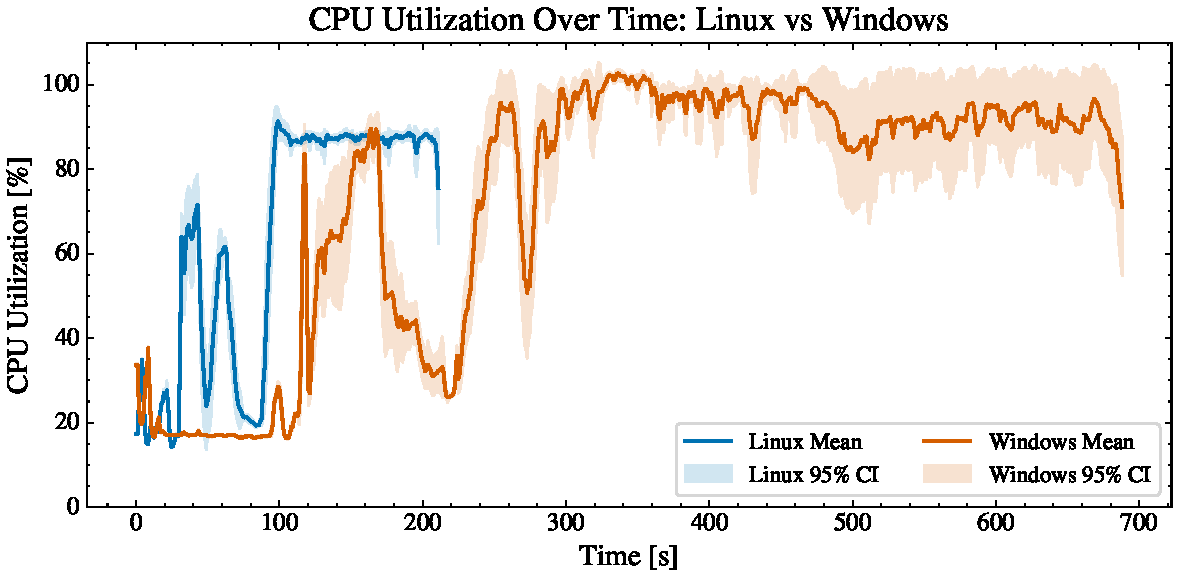
\includegraphics[width=\textwidth]{Messungen/FIFO_500_10T/cpu_timeseries_combined.pdf}
\caption{Zeitlicher Verlauf der \acs{CPU}-Auslastung des \acs{FIFO}\_500-Schedulers auf Linux und Windows bei zehn Threads}
\label{fig:fifo500-10t-cpu-ts}
\end{figure}

\begin{figure}[H]
\centering
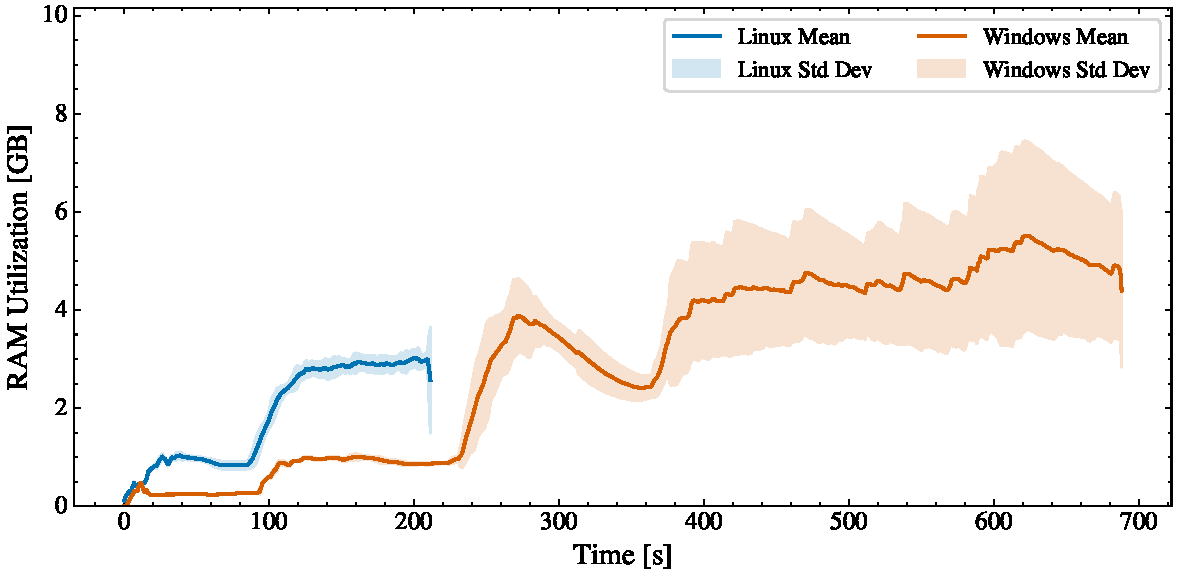
\includegraphics[width=\textwidth]{Messungen/FIFO_500_10T/ram_timeseries_combined.pdf}
\caption{Zeitlicher Verlauf der \acs{RAM}-Auslastung des \acs{FIFO}\_500-Schedulers auf Linux und Windows bei zehn Threads}
\label{fig:fifo500-10t-ram-ts}
\end{figure}

\subsection{Vergleich}
\begin{figure}[H]
\centering
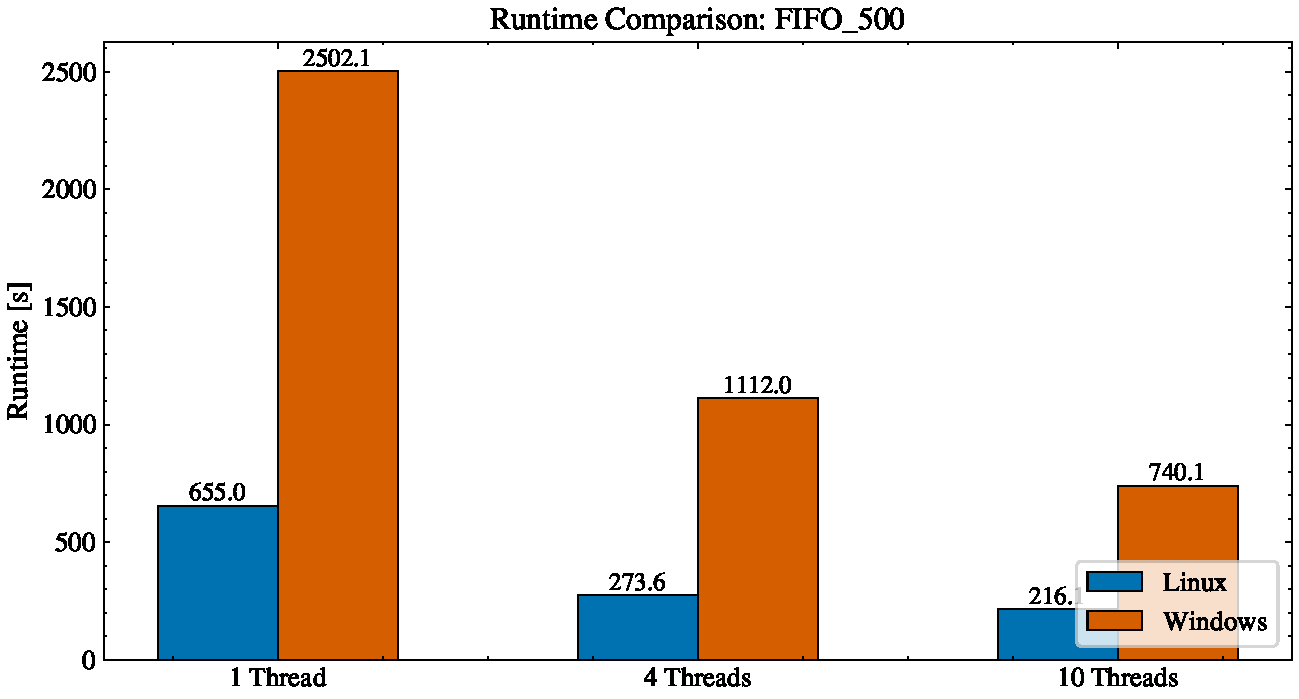
\includegraphics[width=\textwidth]{Messungen/Thread_Comparison/thread_fifo_500_runtime.pdf}
\caption{Vergleich der Laufzeiten des \acs{FIFO}\_500-Schedulers auf Linux und Windows über ein, vier und zehn Threads, dargestellt als Balkendiagramm mit Mittelwerten und Standardabweichungen aus 20 Messläufen}
\label{fig:fifo500-threadcmp-runtime}
\end{figure}

\begin{figure}[H]
\centering
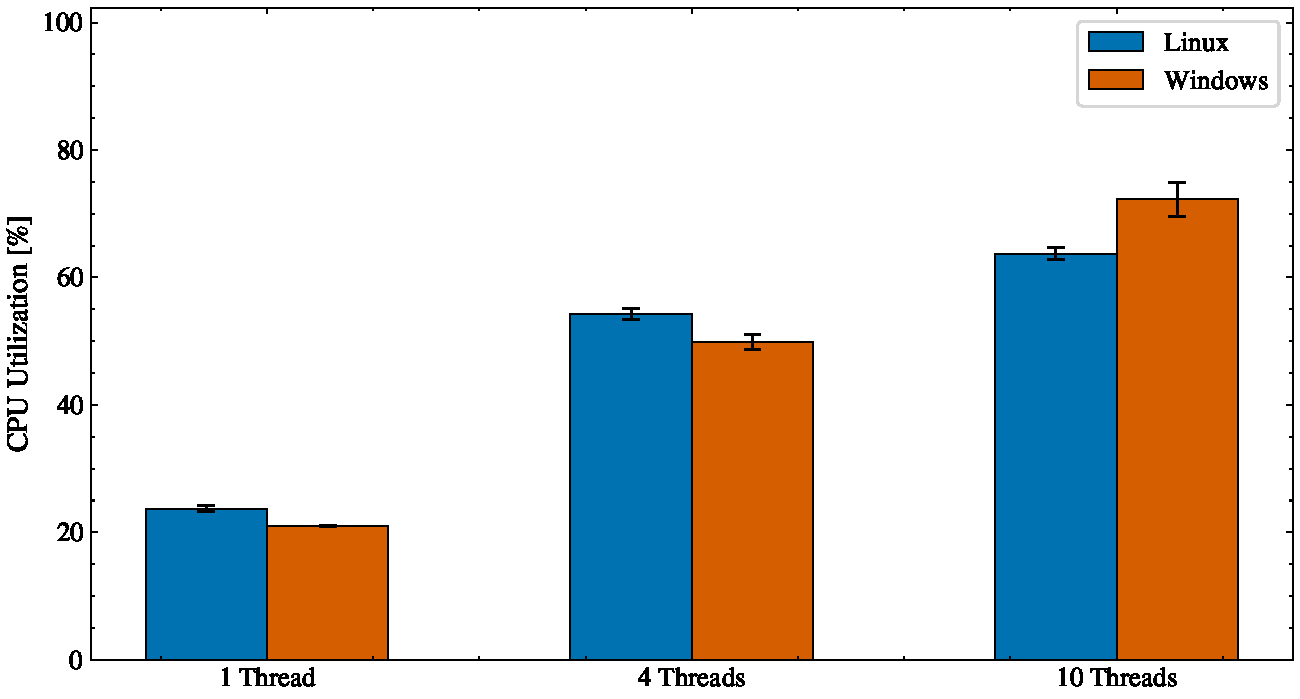
\includegraphics[width=\textwidth]{Messungen/Thread_Comparison/thread_fifo_500_cpu.pdf}
\caption{Vergleich der \acs{CPU}-Auslastung des \acs{FIFO}\_500-Schedulers auf Linux und Windows über ein, vier und zehn Threads, dargestellt als Balkendiagramm mit Mittelwerten und Standardabweichungen aus 20 Messläufen}
\label{fig:fifo500-threadcmp-cpu}
\end{figure}

\begin{figure}[H]
\centering
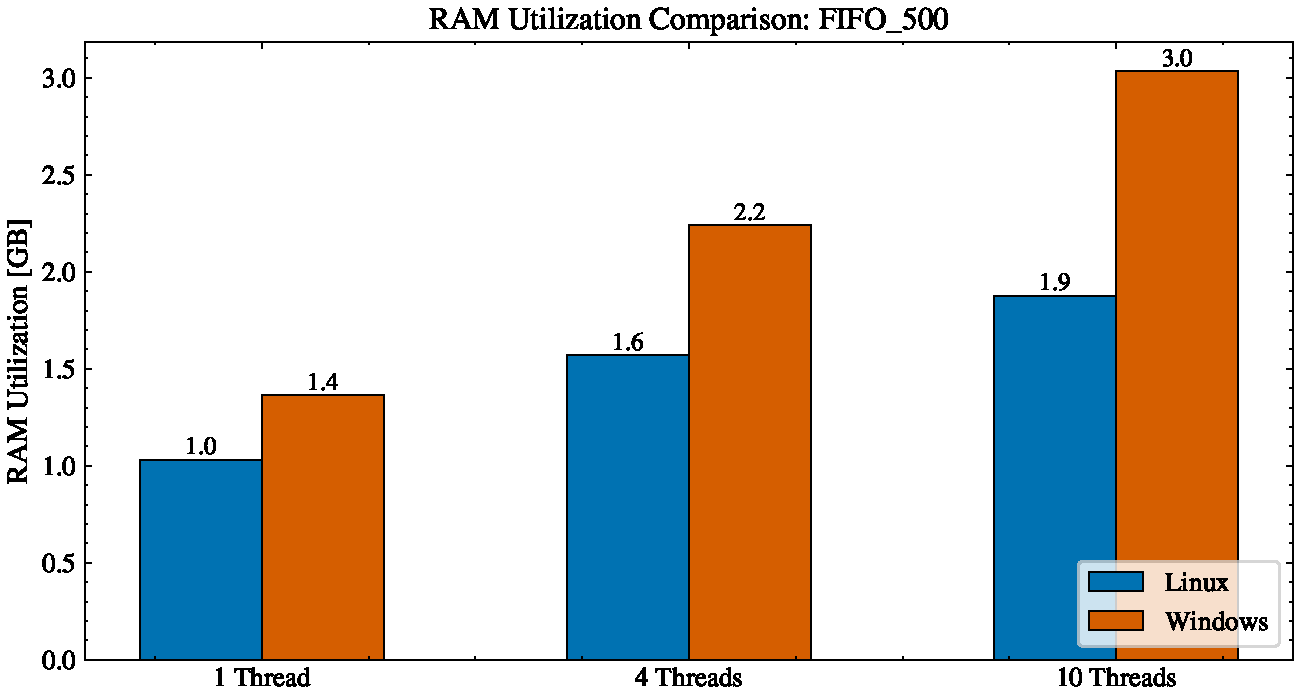
\includegraphics[width=\textwidth]{Messungen/Thread_Comparison/thread_fifo_500_ram.pdf}
\caption{Vergleich der \acs{RAM}-Auslastung des \acs{FIFO}\_500-Schedulers auf Linux und Windows über ein, vier und zehn Threads, dargestellt als Balkendiagramm mit Mittelwerten und Standardabweichungen aus 20 Messläufen}
\label{fig:fifo500-threadcmp-ram}
\end{figure}


\section{Shortest-Subtree-Time-First (\acs{SSTF})}

\subsection{Ein Thread}
\begin{figure}[H]
\centering
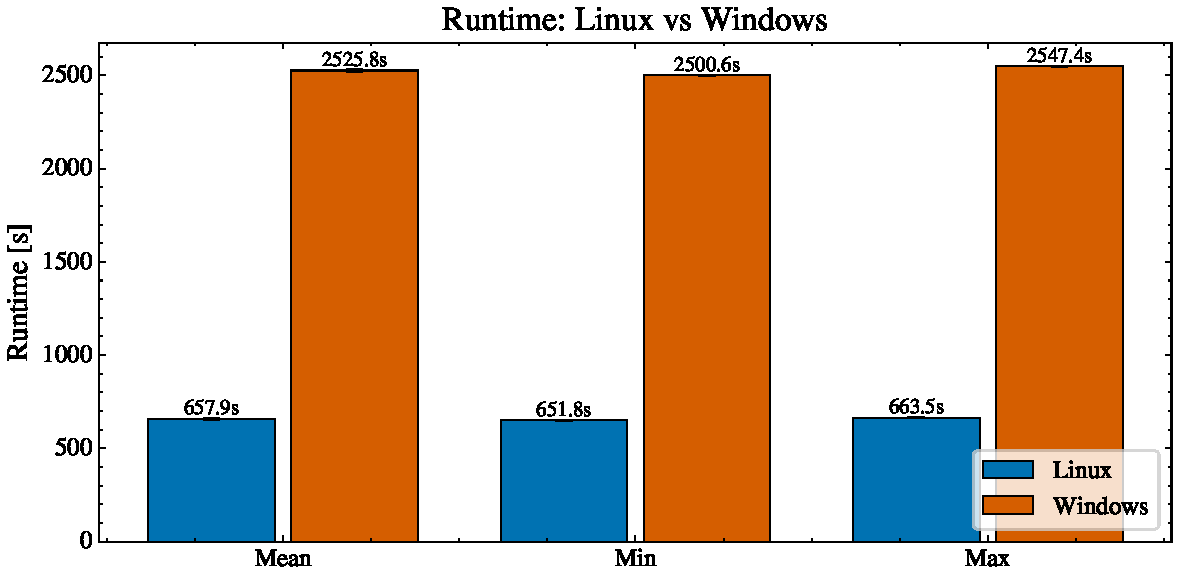
\includegraphics[width=\textwidth]{Messungen/SSTF_1T/runtime_bars_combined.pdf}
\caption{Laufzeiten des \acs{SSTF}-Schedulers auf Linux und Windows bei einem Thread, dargestellt als Balkendiagramm mit Mittelwerten und Standardabweichungen aus 20 Messläufen}
\label{fig:sstf-1t-runtime}
\end{figure}

\begin{figure}[H]
\centering
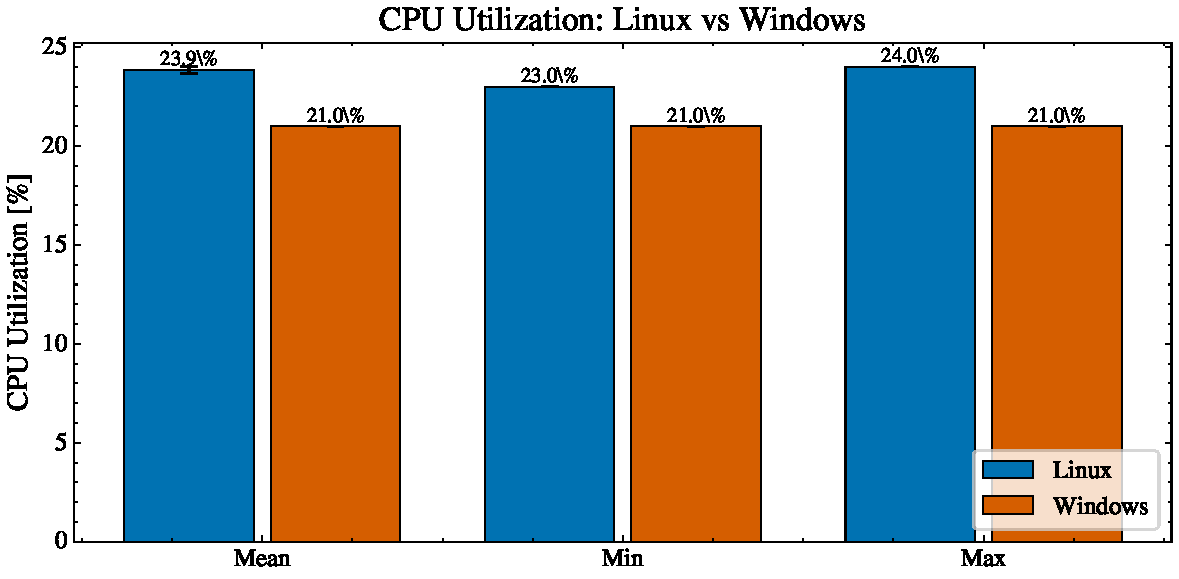
\includegraphics[width=\textwidth]{Messungen/SSTF_1T/cpu_bars_combined.pdf}
\caption{\acs{CPU}-Auslastung des \acs{SSTF}-Schedulers auf Linux und Windows bei einem Thread, dargestellt als Balkendiagramm mit Mittelwerten und Standardabweichungen aus 20 Messläufen}
\label{fig:sstf-1t-cpu}
\end{figure}

\begin{figure}[H]
\centering
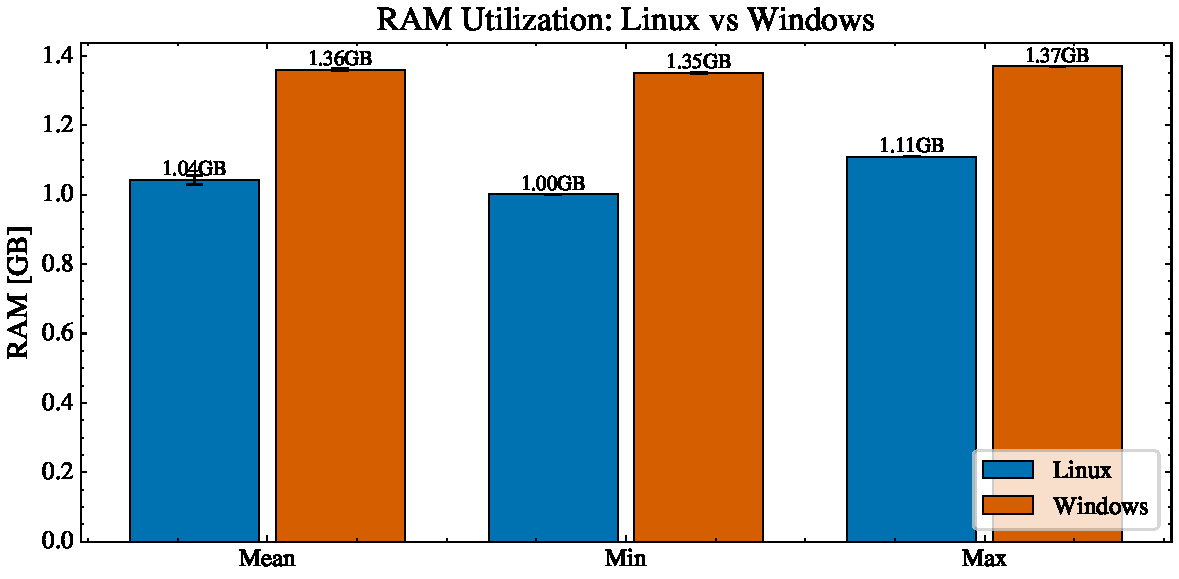
\includegraphics[width=\textwidth]{Messungen/SSTF_1T/ram_bars_combined.pdf}
\caption{\acs{RAM}-Auslastung des \acs{SSTF}-Schedulers auf Linux und Windows bei einem Thread, dargestellt als Balkendiagramm mit Mittelwerten und Standardabweichungen aus 20 Messläufen}
\label{fig:sstf-1t-ram}
\end{figure}

\begin{figure}[H]
\centering
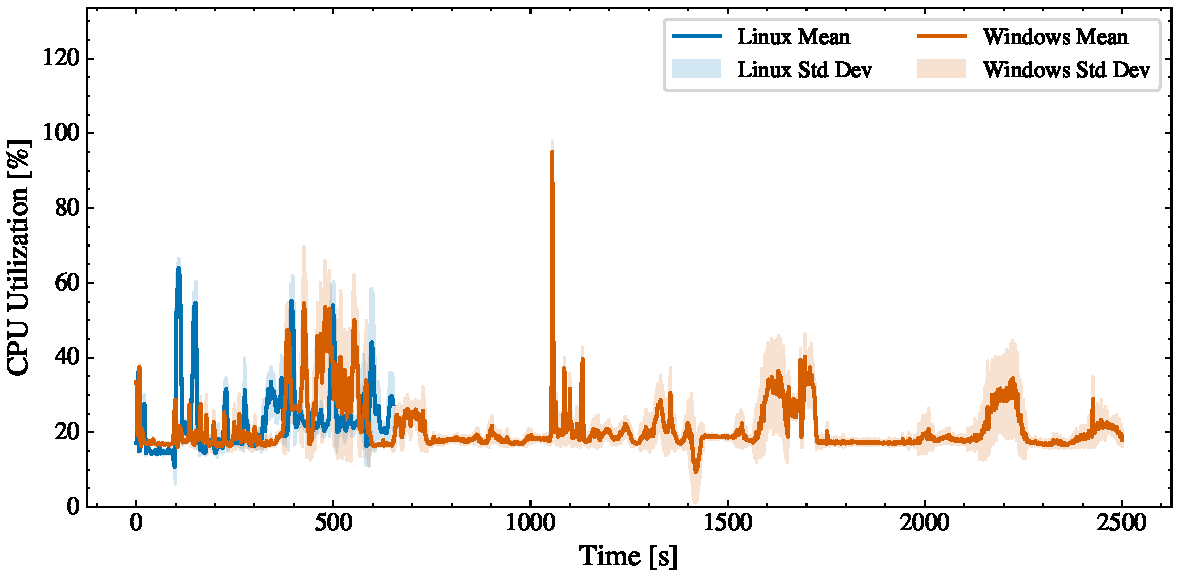
\includegraphics[width=\textwidth]{Messungen/SSTF_1T/cpu_timeseries_combined.pdf}
\caption{Zeitlicher Verlauf der \acs{CPU}-Auslastung des \acs{SSTF}-Schedulers auf Linux und Windows bei einem Thread}
\label{fig:sstf-1t-cpu-ts}
\end{figure}

\begin{figure}[H]
\centering
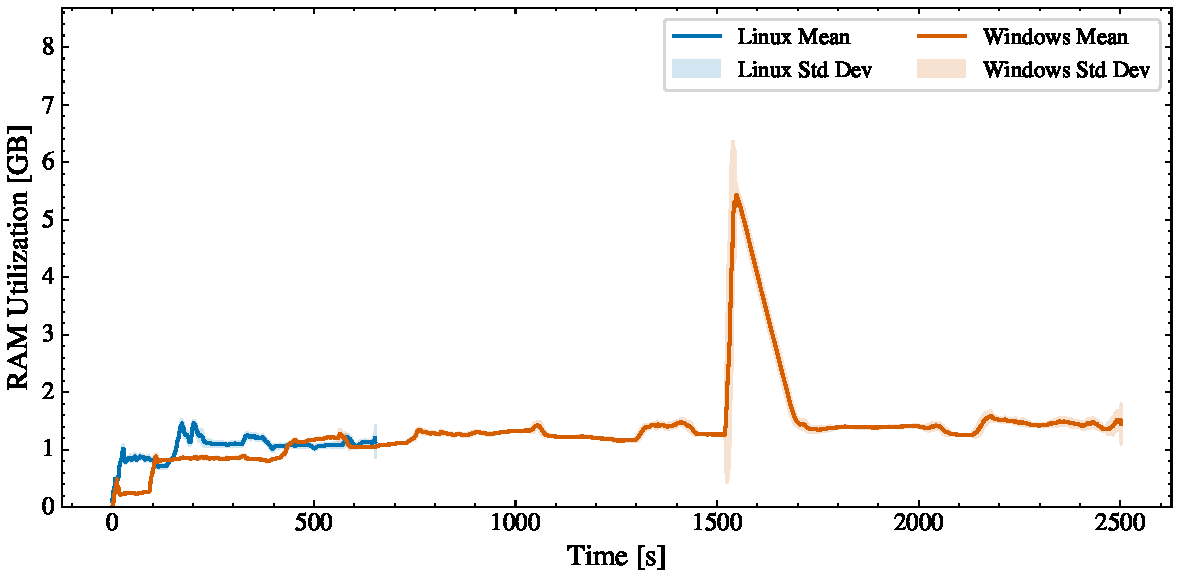
\includegraphics[width=\textwidth]{Messungen/SSTF_1T/ram_timeseries_combined.pdf}
\caption{Zeitlicher Verlauf der \acs{RAM}-Auslastung des \acs{SSTF}-Schedulers auf Linux und Windows bei einem Thread}
\label{fig:sstf-1t-ram-ts}
\end{figure}

\subsection{Vier Threads}
\begin{figure}[H]
\centering
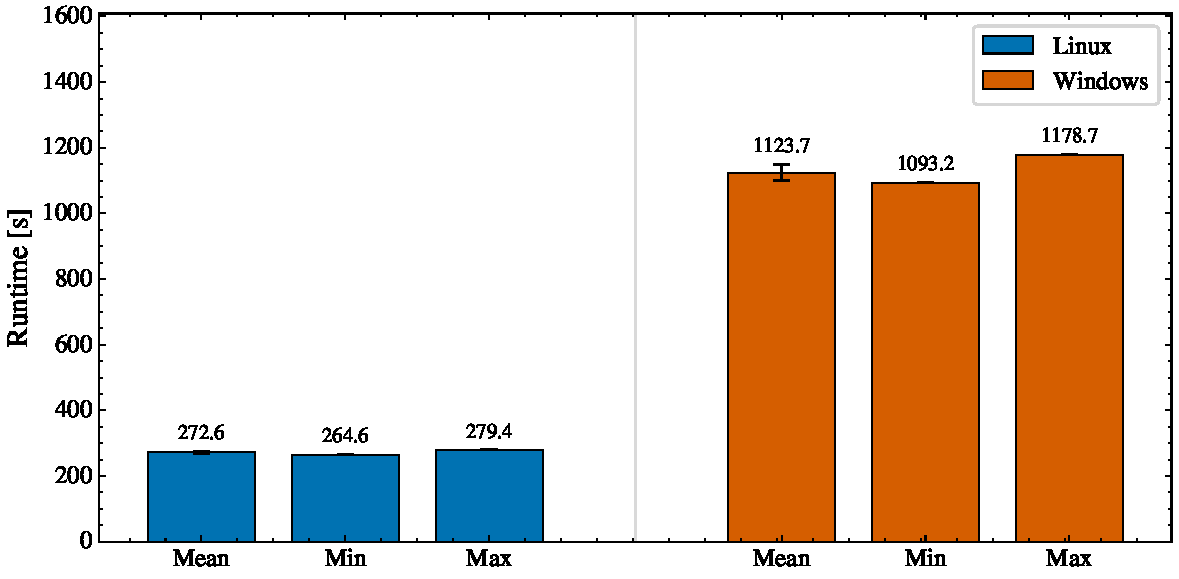
\includegraphics[width=\textwidth]{Messungen/SSTF_4T/runtime_bars_combined.pdf}
\caption{Laufzeiten des \acs{SSTF}-Schedulers auf Linux und Windows bei vier Threads, dargestellt als Balkendiagramm mit Mittelwerten und Standardabweichungen aus 20 Messläufen}
\label{fig:sstf-4t-runtime}
\end{figure}

\begin{figure}[H]
\centering
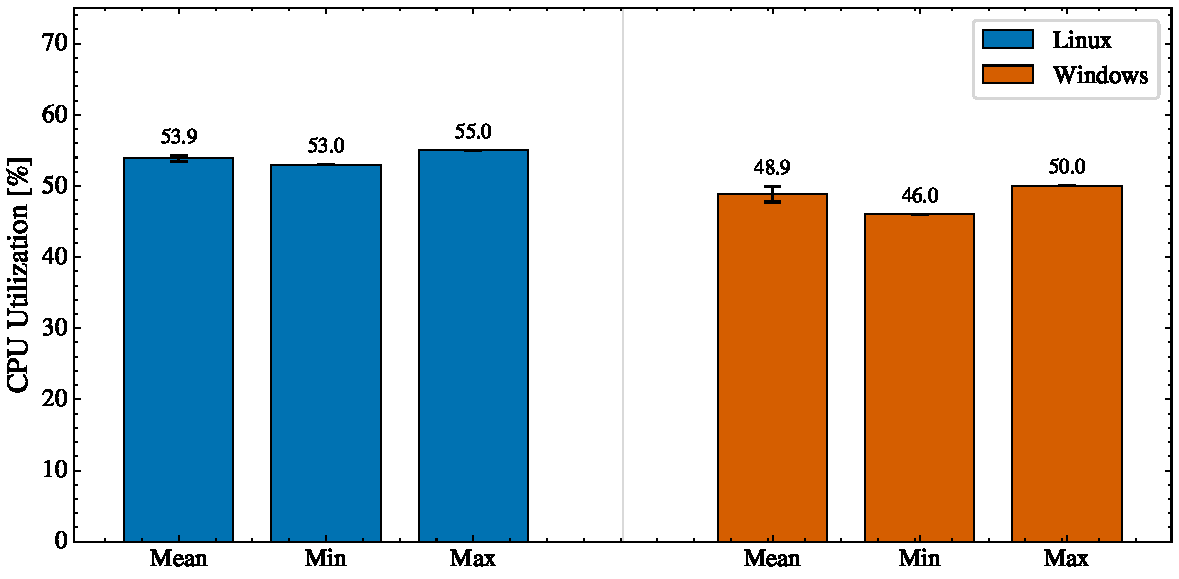
\includegraphics[width=\textwidth]{Messungen/SSTF_4T/cpu_bars_combined.pdf}
\caption{\acs{CPU}-Auslastung des \acs{SSTF}-Schedulers auf Linux und Windows bei vier Threads, dargestellt als Balkendiagramm mit Mittelwerten und Standardabweichungen aus 20 Messläufen}
\label{fig:sstf-4t-cpu}
\end{figure}

\begin{figure}[H]
\centering
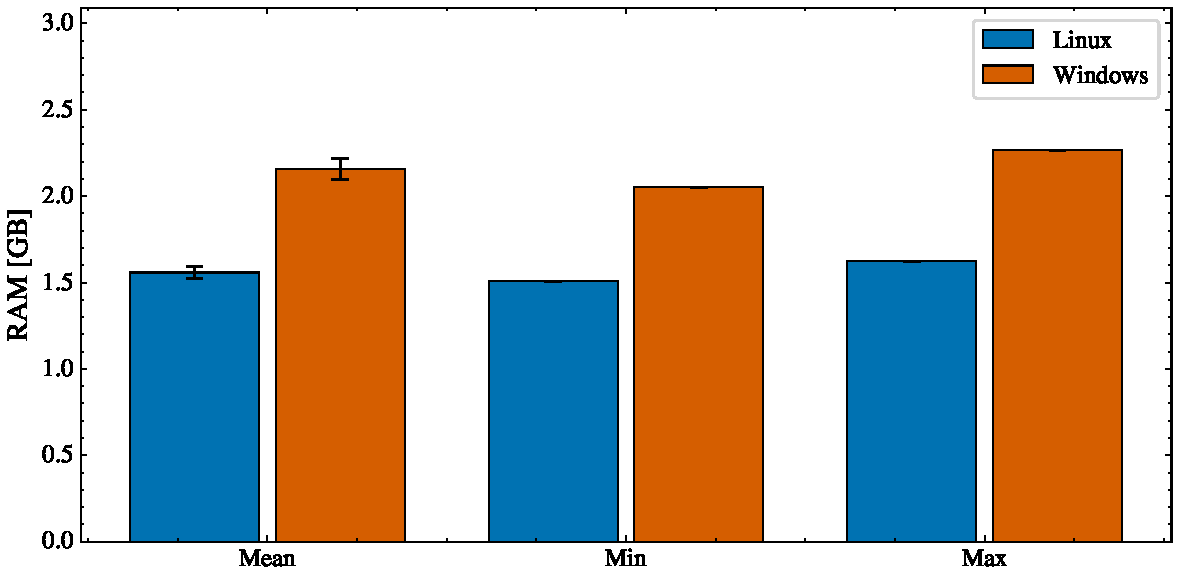
\includegraphics[width=\textwidth]{Messungen/SSTF_4T/ram_bars_combined.pdf}
\caption{\acs{RAM}-Auslastung des \acs{SSTF}-Schedulers auf Linux und Windows bei vier Threads, dargestellt als Balkendiagramm mit Mittelwerten und Standardabweichungen aus 20 Messläufen}
\label{fig:sstf-4t-ram}
\end{figure}

\begin{figure}[H]
\centering
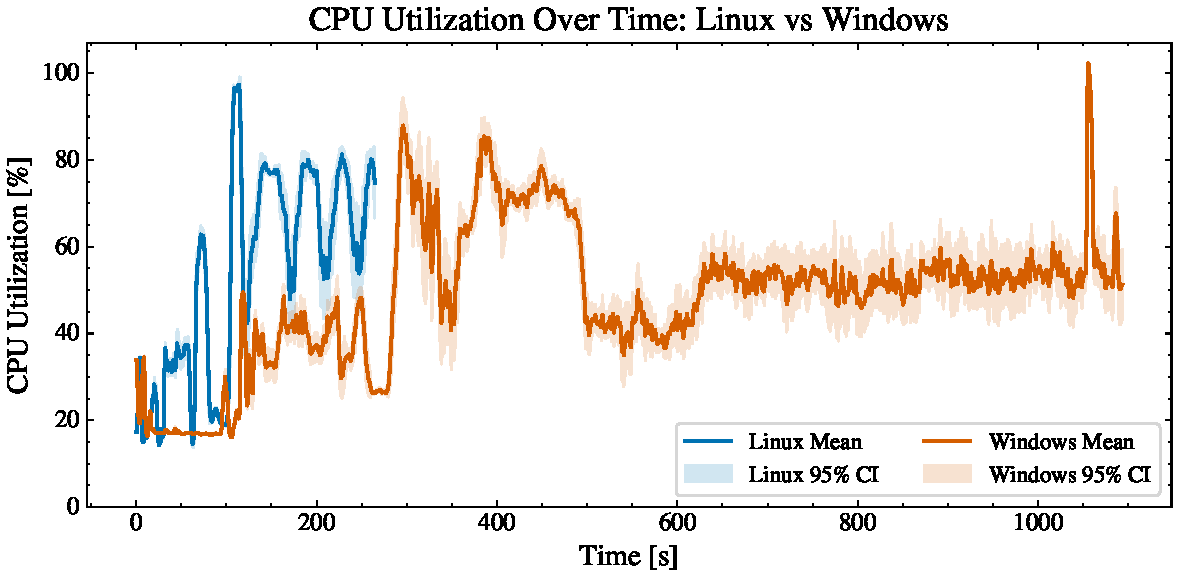
\includegraphics[width=\textwidth]{Messungen/SSTF_4T/cpu_timeseries_combined.pdf}
\caption{Zeitlicher Verlauf der \acs{CPU}-Auslastung des \acs{SSTF}-Schedulers auf Linux und Windows bei vier Threads}
\label{fig:sstf-4t-cpu-ts}
\end{figure}

\begin{figure}[H]
\centering
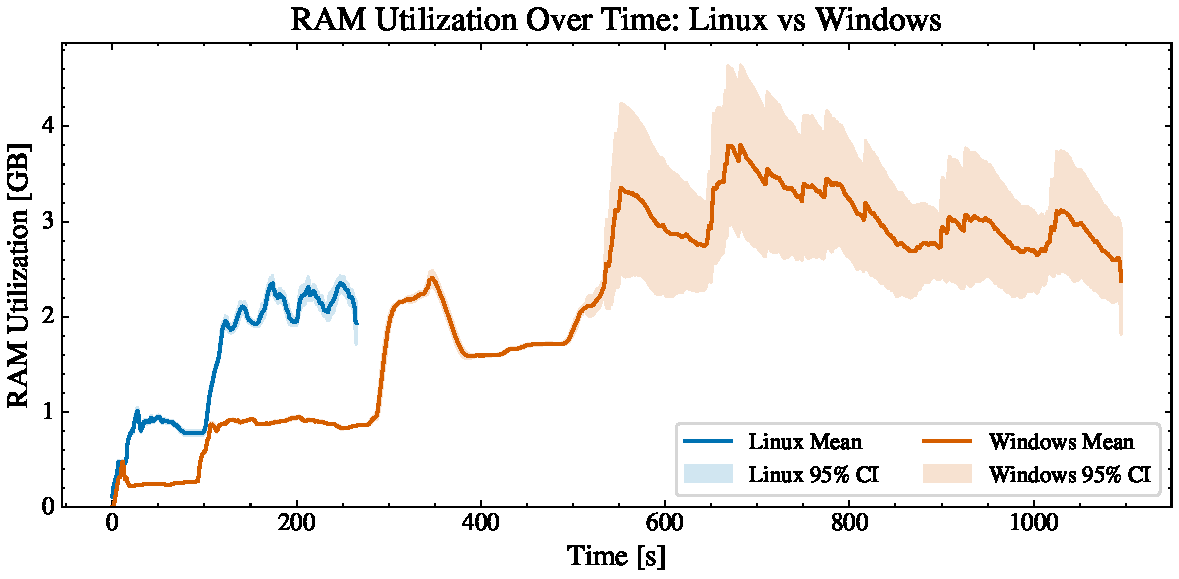
\includegraphics[width=\textwidth]{Messungen/SSTF_4T/ram_timeseries_combined.pdf}
\caption{Zeitlicher Verlauf der \acs{RAM}-Auslastung des \acs{SSTF}-Schedulers auf Linux und Windows bei vier Threads}
\label{fig:sstf-4t-ram-ts}
\end{figure}

\subsection{Zehn Threads}
\begin{figure}[H]
\centering
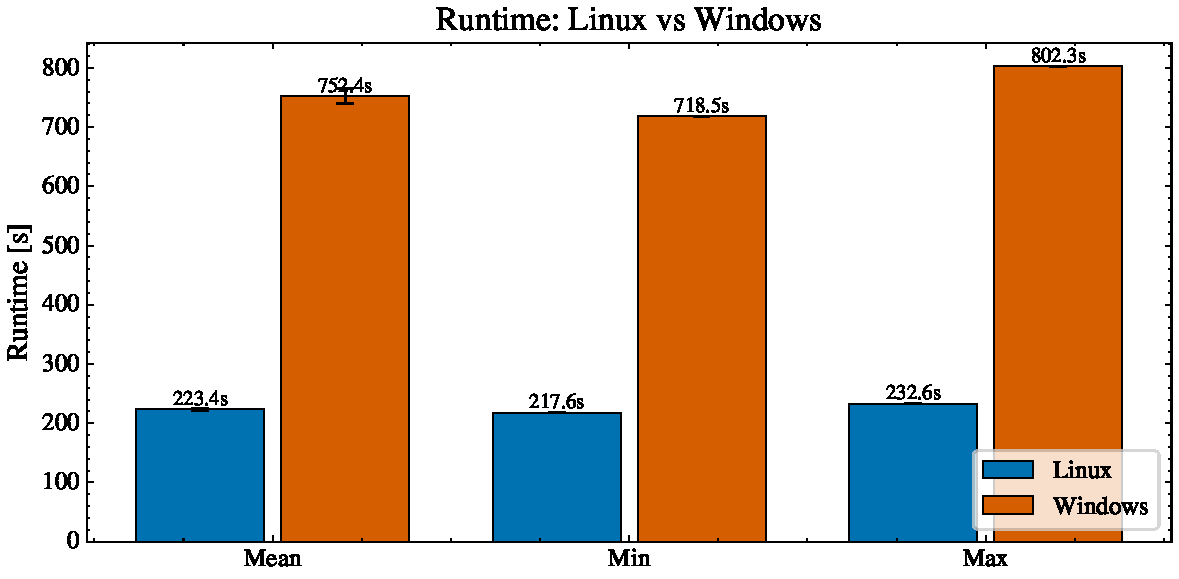
\includegraphics[width=\textwidth]{Messungen/SSTF_10T/runtime_bars_combined.pdf}
\caption{Laufzeiten des \acs{SSTF}-Schedulers auf Linux und Windows bei zehn Threads, dargestellt als Balkendiagramm mit Mittelwerten und Standardabweichungen aus 20 Messläufen}
\label{fig:sstf-10t-runtime}
\end{figure}

\begin{figure}[H]
\centering
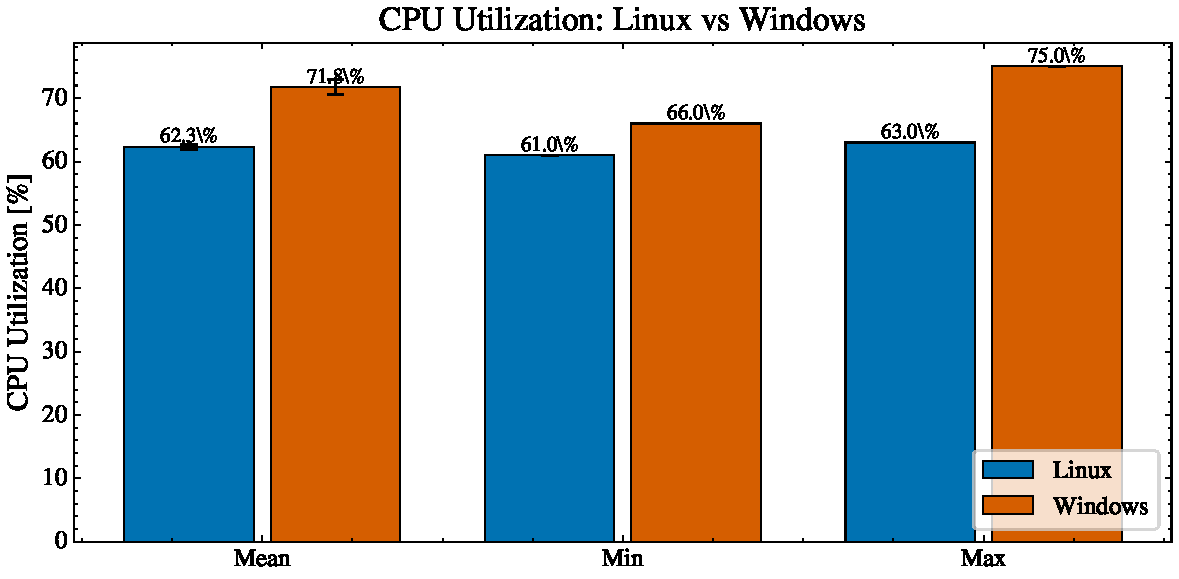
\includegraphics[width=\textwidth]{Messungen/SSTF_10T/cpu_bars_combined.pdf}
\caption{\acs{CPU}-Auslastung des \acs{SSTF}-Schedulers auf Linux und Windows bei zehn Threads, dargestellt als Balkendiagramm mit Mittelwerten und Standardabweichungen aus 20 Messläufen}
\label{fig:sstf-10t-cpu}
\end{figure}

\begin{figure}[H]
\centering
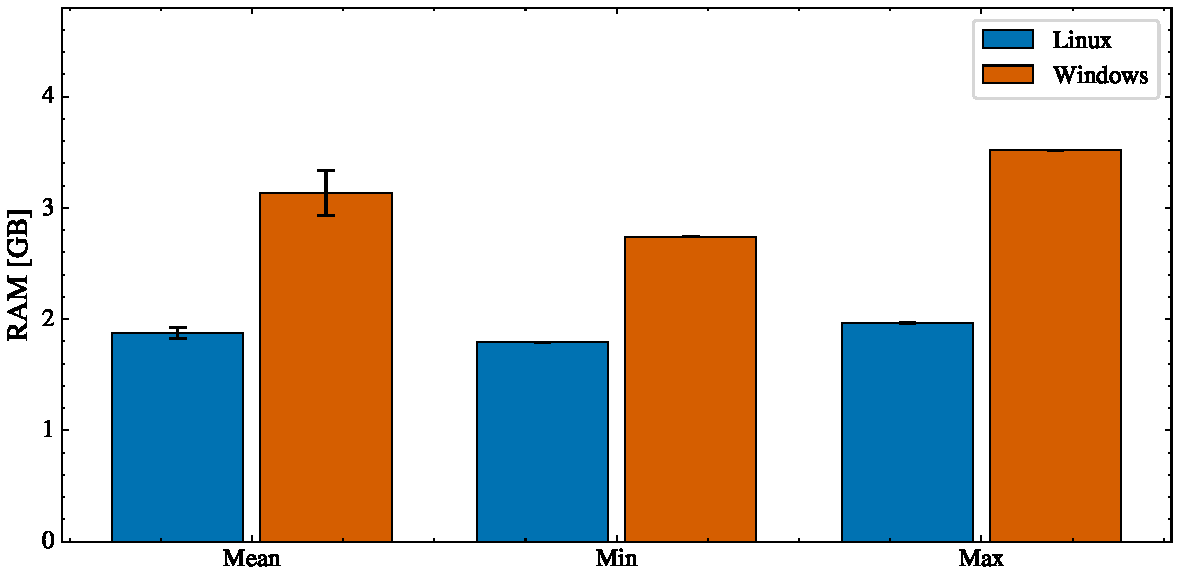
\includegraphics[width=\textwidth]{Messungen/SSTF_10T/ram_bars_combined.pdf}
\caption{\acs{RAM}-Auslastung des \acs{SSTF}-Schedulers auf Linux und Windows bei zehn Threads, dargestellt als Balkendiagramm mit Mittelwerten und Standardabweichungen aus 20 Messläufen}
\label{fig:sstf-10t-ram}
\end{figure}

\begin{figure}[H]
\centering
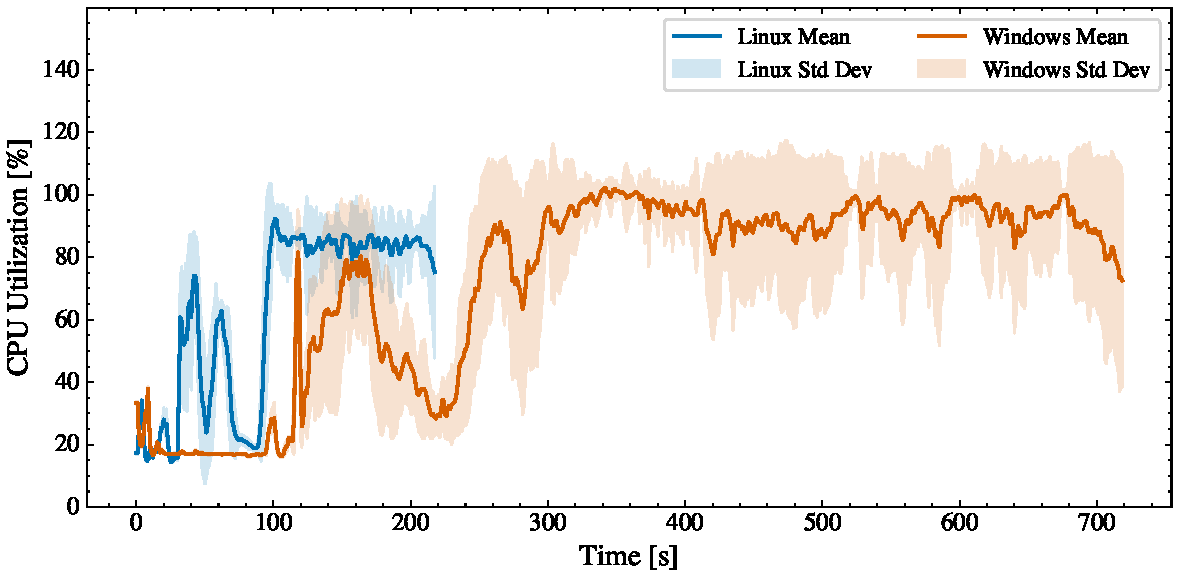
\includegraphics[width=\textwidth]{Messungen/SSTF_10T/cpu_timeseries_combined.pdf}
\caption{Zeitlicher Verlauf der \acs{CPU}-Auslastung des \acs{SSTF}-Schedulers auf Linux und Windows bei zehn Threads}
\label{fig:sstf-10t-cpu-ts}
\end{figure}

\begin{figure}[H]
\centering
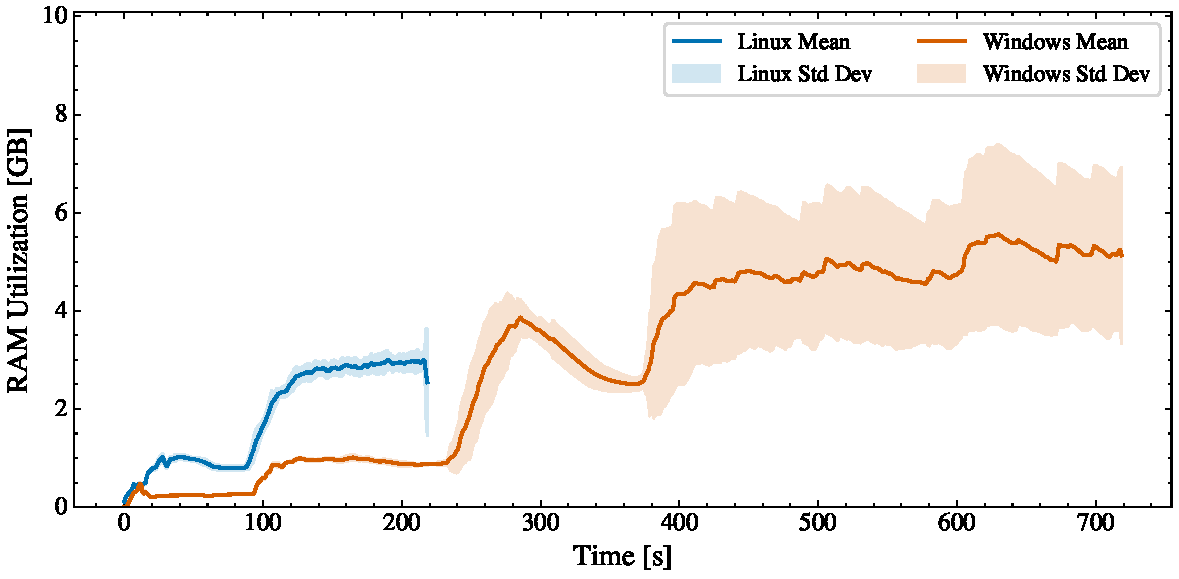
\includegraphics[width=\textwidth]{Messungen/SSTF_10T/ram_timeseries_combined.pdf}
\caption{Zeitlicher Verlauf der \acs{RAM}-Auslastung des \acs{SSTF}-Schedulers auf Linux und Windows bei zehn Threads}
\label{fig:sstf-10t-ram-ts}
\end{figure}

\subsection{Vergleich}
\begin{figure}[H]
\centering
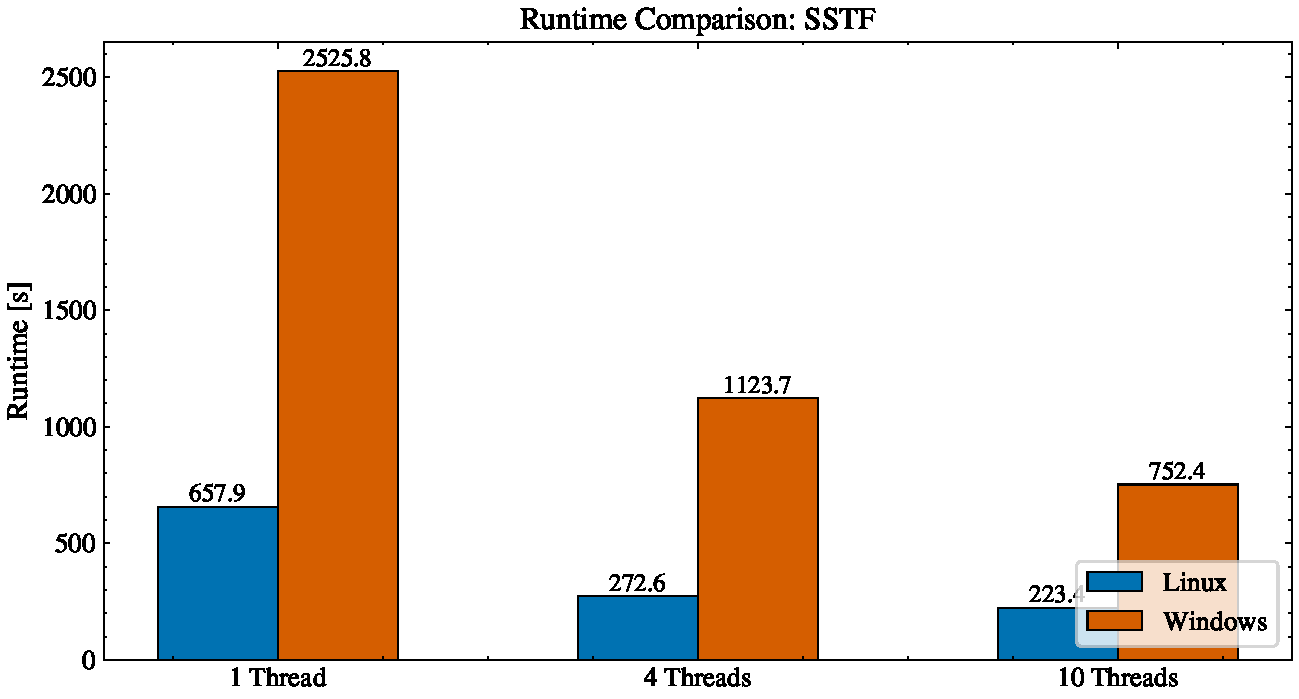
\includegraphics[width=\textwidth]{Messungen/Thread_Comparison/thread_sstf_runtime.pdf}
\caption{Vergleich der Laufzeiten des \acs{SSTF}-Schedulers auf Linux und Windows über ein, vier und zehn Threads, dargestellt als Balkendiagramm mit Mittelwerten und Standardabweichungen aus 20 Messläufen}
\label{fig:sstf-threadcmp-runtime}
\end{figure}

\begin{figure}[H]
\centering
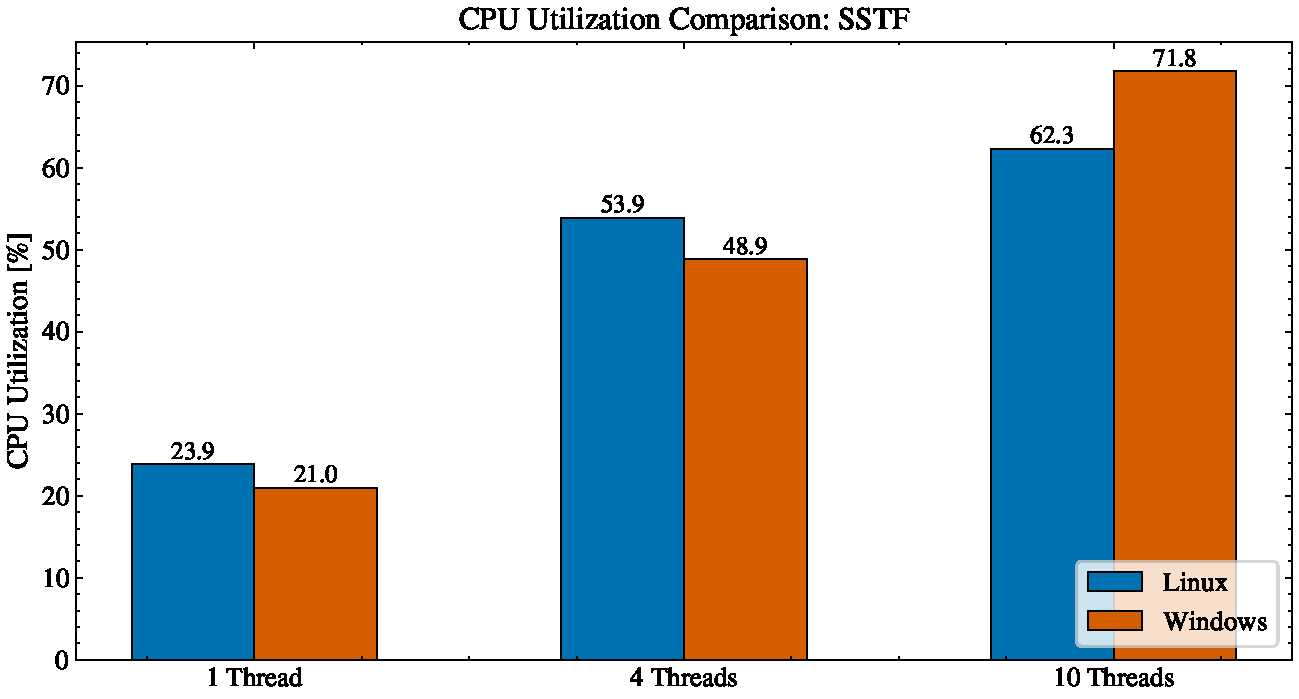
\includegraphics[width=\textwidth]{Messungen/Thread_Comparison/thread_sstf_cpu.pdf}
\caption{Vergleich der \acs{CPU}-Auslastung des \acs{SSTF}-Schedulers auf Linux und Windows über ein, vier und zehn Threads, dargestellt als Balkendiagramm mit Mittelwerten und Standardabweichungen aus 20 Messläufen}
\label{fig:sstf-threadcmp-cpu}
\end{figure}

\begin{figure}[H]
\centering
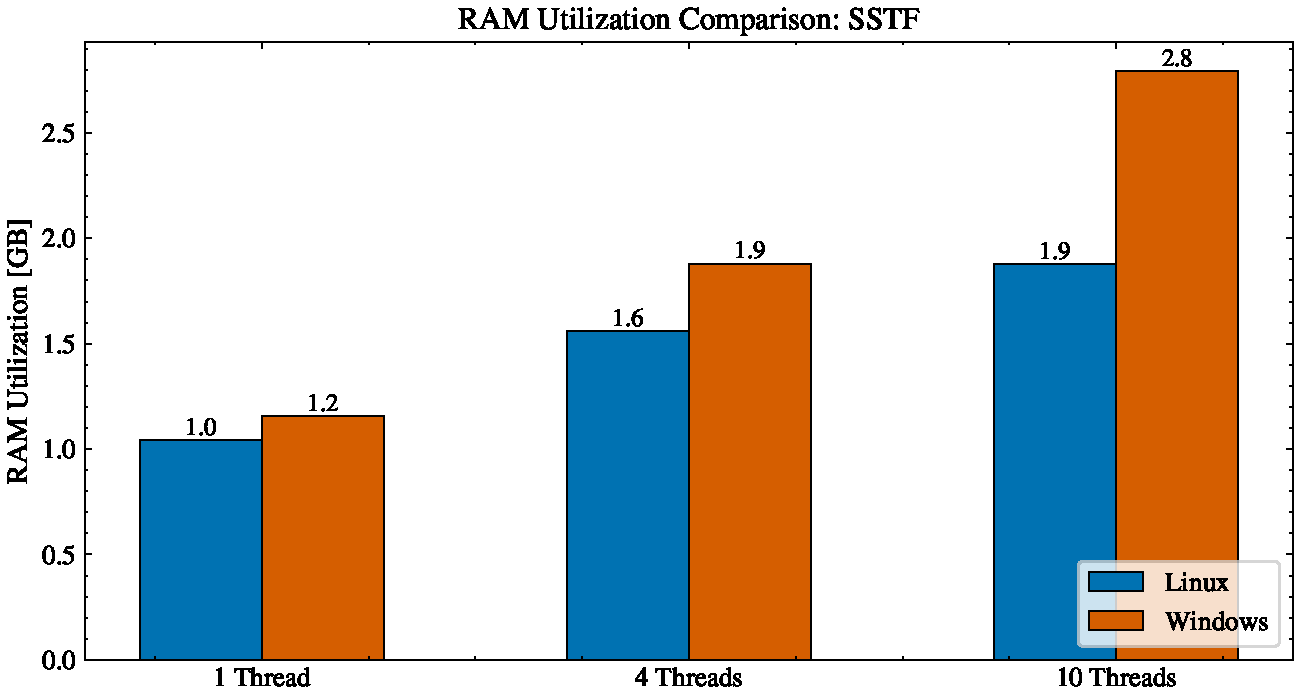
\includegraphics[width=\textwidth]{Messungen/Thread_Comparison/thread_sstf_ram.pdf}
\caption{Vergleich der \acs{RAM}-Auslastung des \acs{SSTF}-Schedulers auf Linux und Windows über ein, vier und zehn Threads, dargestellt als Balkendiagramm mit Mittelwerten und Standardabweichungen aus 20 Messläufen}
\label{fig:sstf-threadcmp-ram}
\end{figure}


\section{Work-Stealing mit \acs{SSTF}-Priorisierung}

\subsection{Ein Thread}
\begin{figure}[H]
\centering
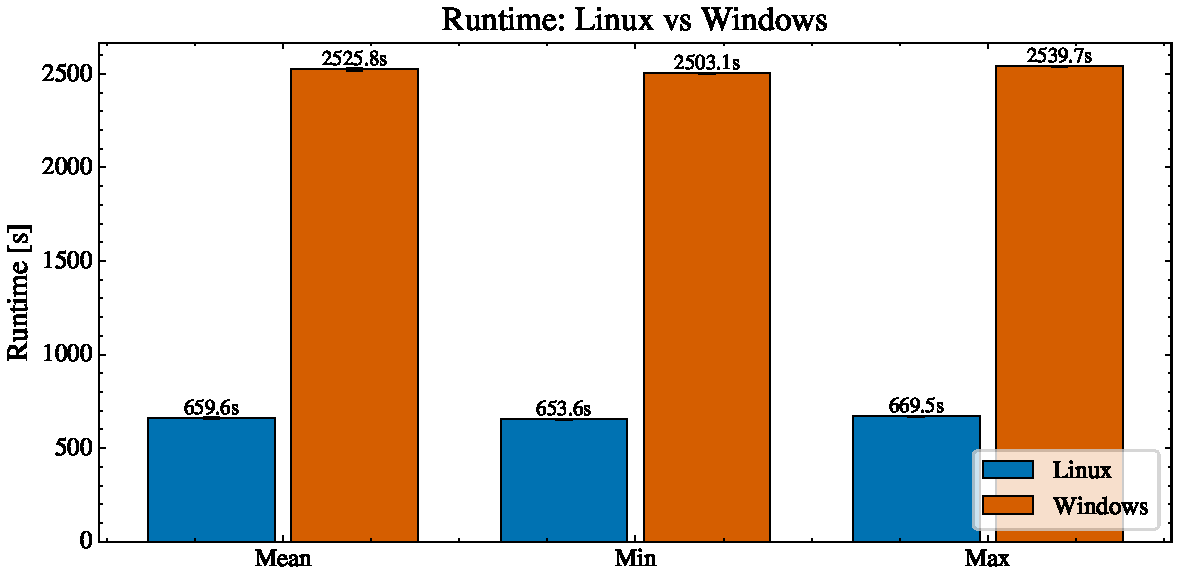
\includegraphics[width=\textwidth]{Messungen/WS_1T/runtime_bars_combined.pdf}
\caption{Laufzeiten des Work-Stealing-Schedulers mit \acs{SSTF}-Priorisierung auf Linux und Windows bei einem Thread, dargestellt als Balkendiagramm mit Mittelwerten und Standardabweichungen aus 20 Messläufen}
\label{fig:ws-1t-runtime}
\end{figure}

\begin{figure}[H]
\centering
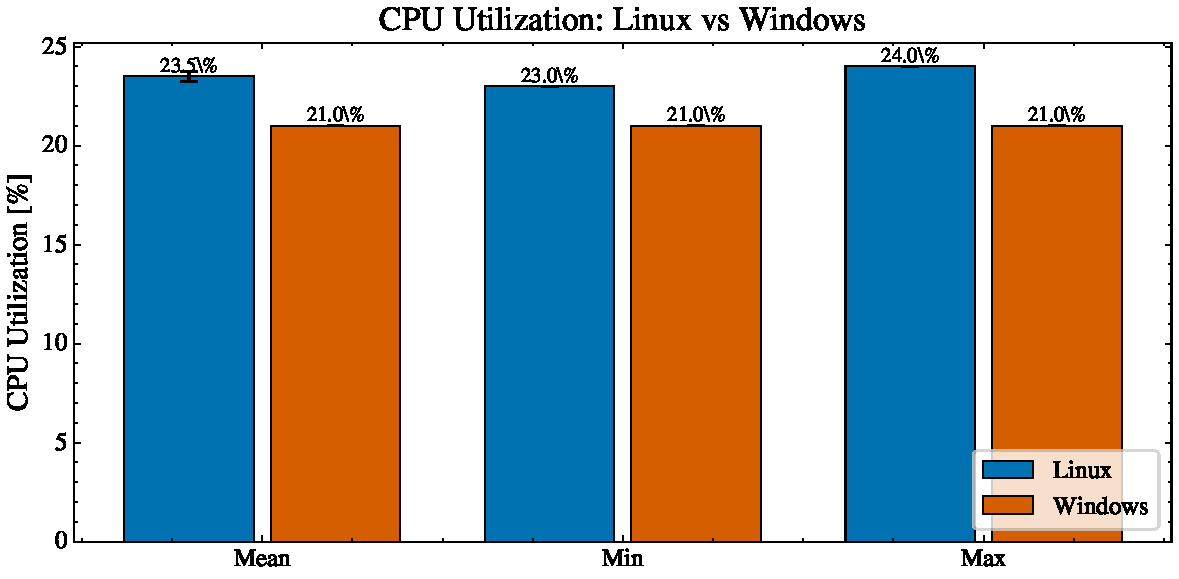
\includegraphics[width=\textwidth]{Messungen/WS_1T/cpu_bars_combined.pdf}
\caption{\acs{CPU}-Auslastung des Work-Stealing-Schedulers mit \acs{SSTF}-Priorisierung auf Linux und Windows bei einem Thread, dargestellt als Balkendiagramm mit Mittelwerten und Standardabweichungen aus 20 Messläufen}
\label{fig:ws-1t-cpu}
\end{figure}

\begin{figure}[H]
\centering
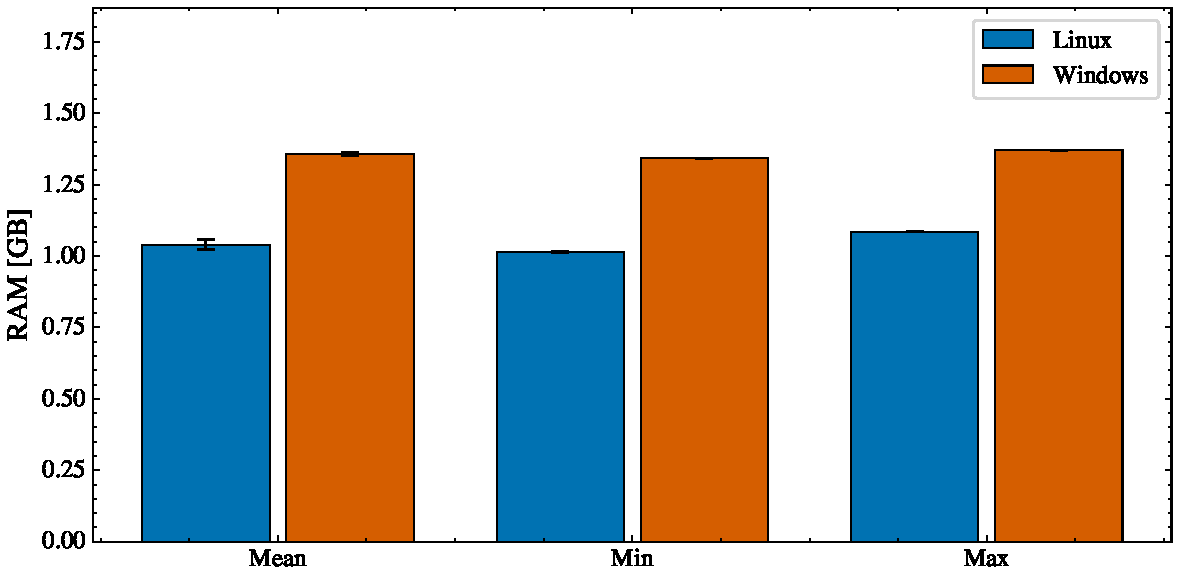
\includegraphics[width=\textwidth]{Messungen/WS_1T/ram_bars_combined.pdf}
\caption{\acs{RAM}-Auslastung des Work-Stealing-Schedulers mit \acs{SSTF}-Priorisierung auf Linux und Windows bei einem Thread, dargestellt als Balkendiagramm mit Mittelwerten und Standardabweichungen aus 20 Messläufen}
\label{fig:ws-1t-ram}
\end{figure}

\begin{figure}[H]
\centering
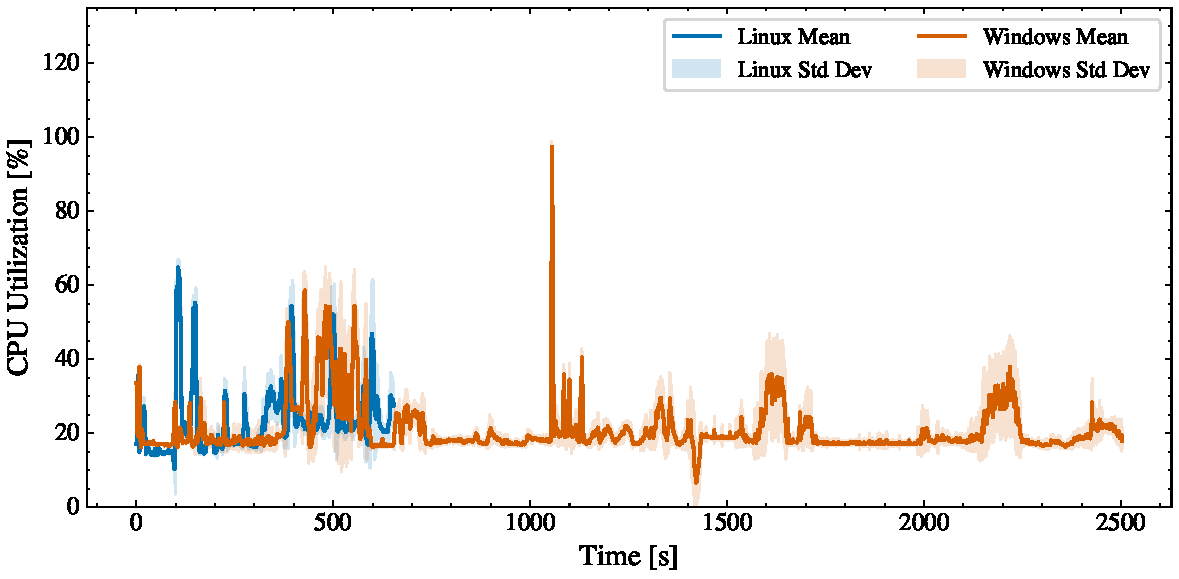
\includegraphics[width=\textwidth]{Messungen/WS_1T/cpu_timeseries_combined.pdf}
\caption{Zeitlicher Verlauf der \acs{CPU}-Auslastung des Work-Stealing-Schedulers mit \acs{SSTF}-Priorisierung auf Linux und Windows bei einem Thread}
\label{fig:ws-1t-cpu-ts}
\end{figure}

\begin{figure}[H]
\centering
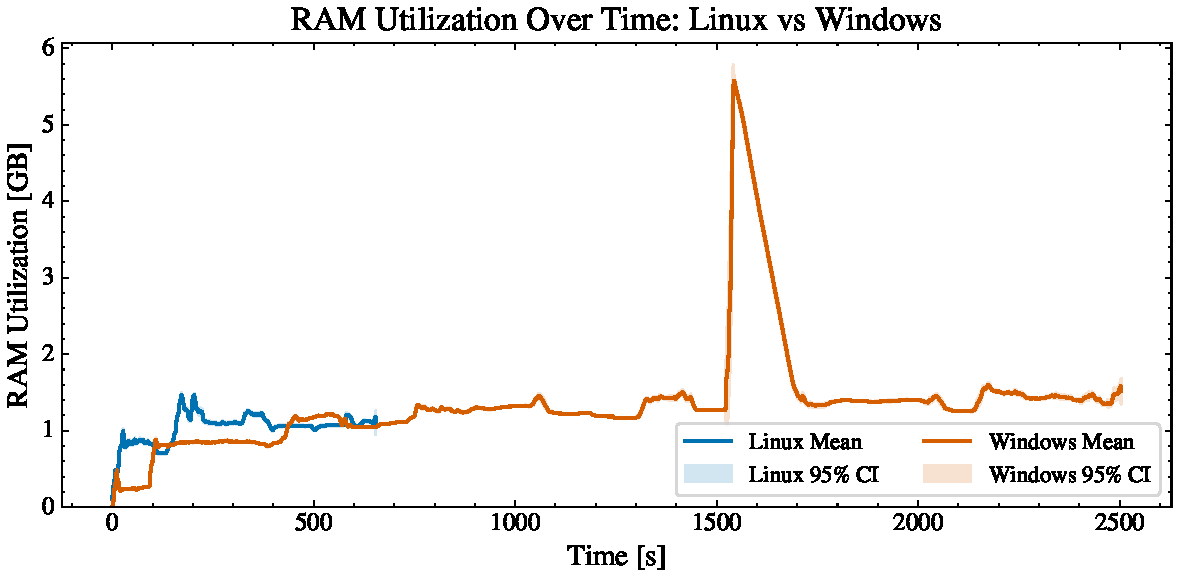
\includegraphics[width=\textwidth]{Messungen/WS_1T/ram_timeseries_combined.pdf}
\caption{Zeitlicher Verlauf der \acs{RAM}-Auslastung des Work-Stealing-Schedulers mit \acs{SSTF}-Priorisierung auf Linux und Windows bei einem Thread}
\label{fig:ws-1t-ram-ts}
\end{figure}

\subsection{Vier Threads}
\begin{figure}[H]
\centering
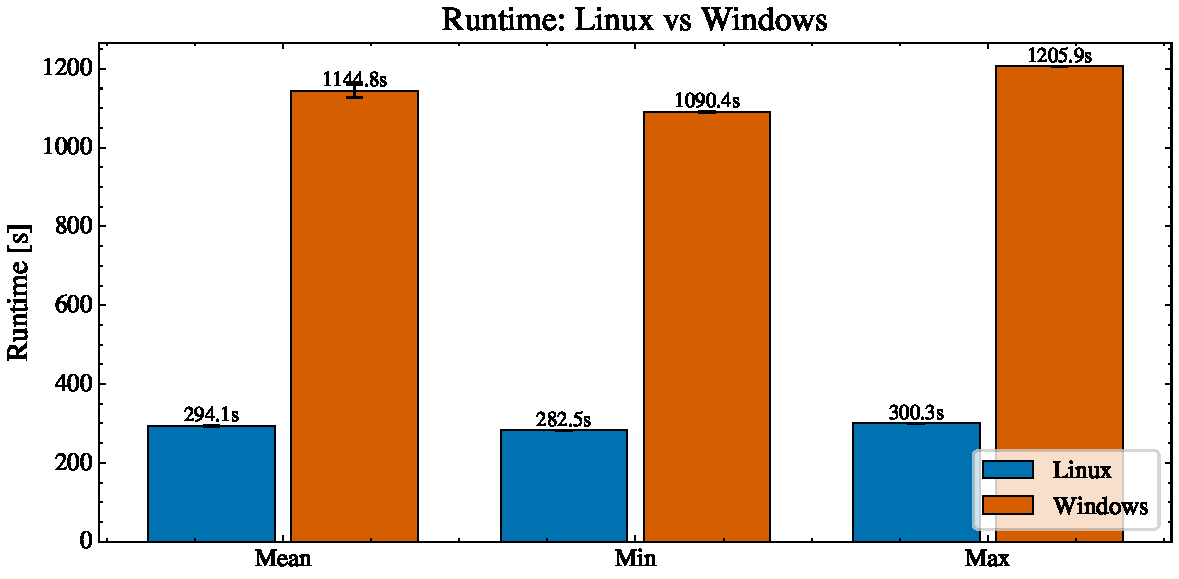
\includegraphics[width=\textwidth]{Messungen/WS_4T/runtime_bars_combined.pdf}
\caption{Laufzeiten des Work-Stealing-Schedulers mit \acs{SSTF}-Priorisierung auf Linux und Windows bei vier Threads, dargestellt als Balkendiagramm mit Mittelwerten und Standardabweichungen aus 20 Messläufen}
\label{fig:ws-4t-runtime}
\end{figure}

\begin{figure}[H]
\centering
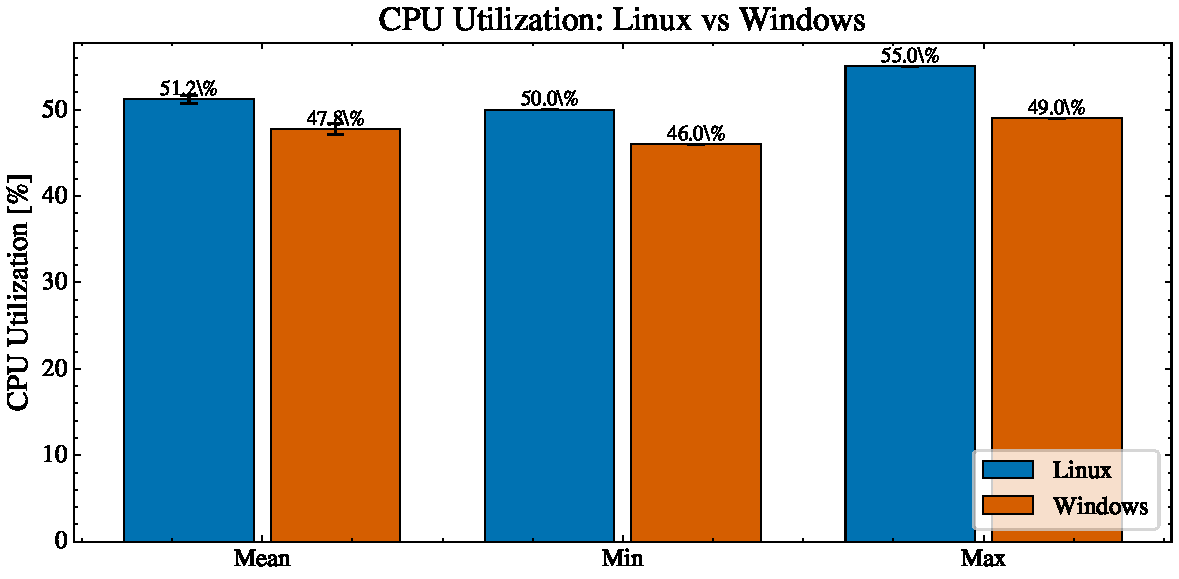
\includegraphics[width=\textwidth]{Messungen/WS_4T/cpu_bars_combined.pdf}
\caption{\acs{CPU}-Auslastung des Work-Stealing-Schedulers mit \acs{SSTF}-Priorisierung auf Linux und Windows bei vier Threads, dargestellt als Balkendiagramm mit Mittelwerten und Standardabweichungen aus 20 Messläufen}
\label{fig:ws-4t-cpu}
\end{figure}

\begin{figure}[H]
\centering
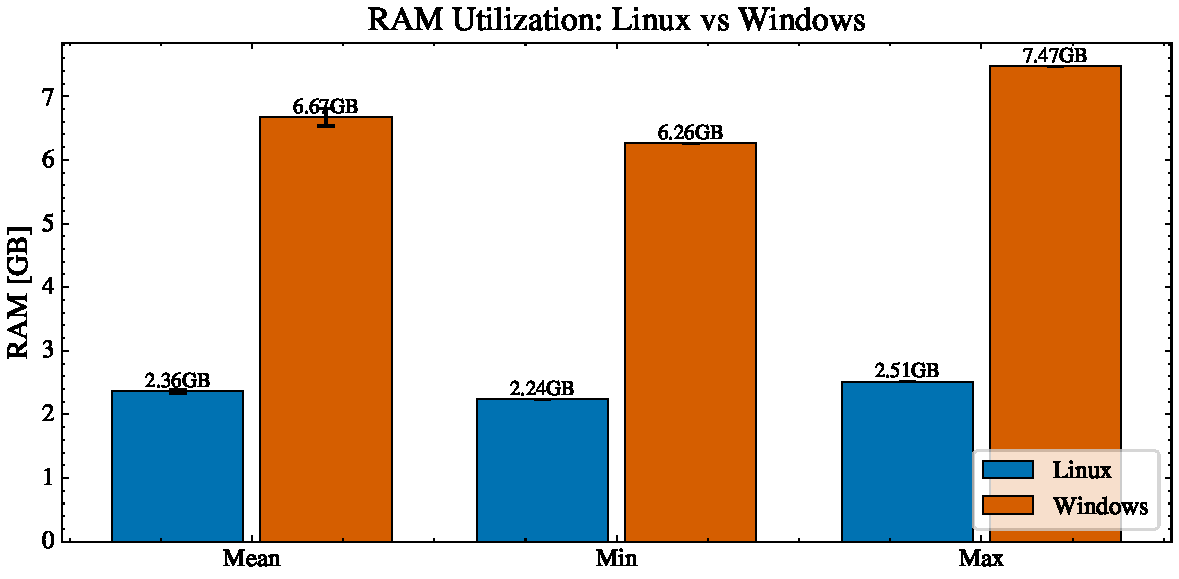
\includegraphics[width=\textwidth]{Messungen/WS_4T/ram_bars_combined.pdf}
\caption{\acs{RAM}-Auslastung des Work-Stealing-Schedulers mit \acs{SSTF}-Priorisierung auf Linux und Windows bei vier Threads, dargestellt als Balkendiagramm mit Mittelwerten und Standardabweichungen aus 20 Messläufen}
\label{fig:ws-4t-ram}
\end{figure}

\begin{figure}[H]
\centering
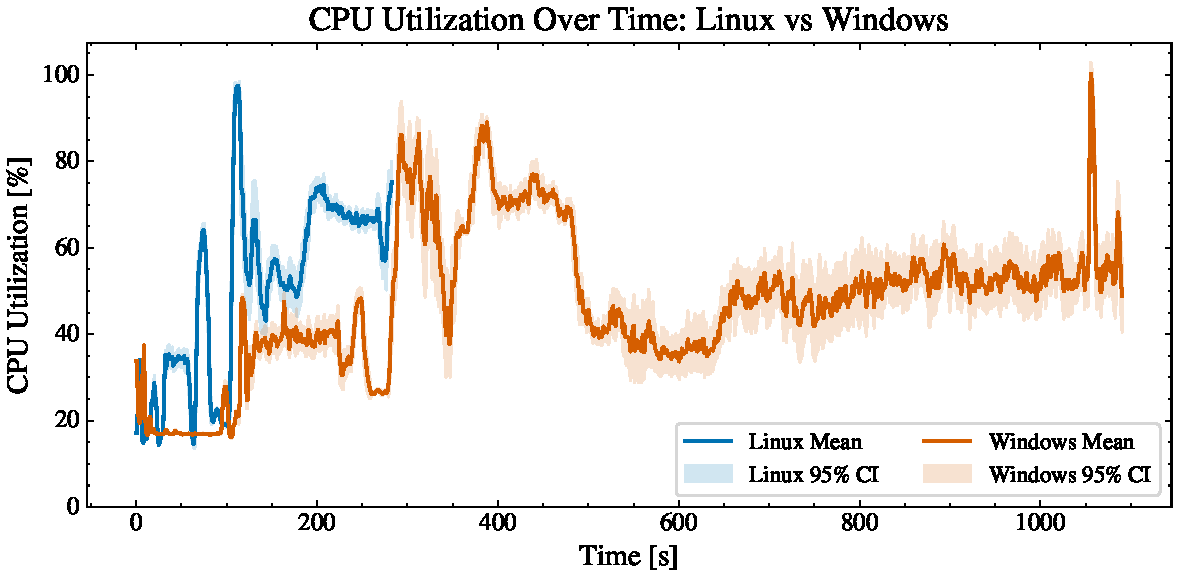
\includegraphics[width=\textwidth]{Messungen/WS_4T/cpu_timeseries_combined.pdf}
\caption{Zeitlicher Verlauf der \acs{CPU}-Auslastung des Work-Stealing-Schedulers mit \acs{SSTF}-Priorisierung auf Linux und Windows bei vier Threads}
\label{fig:ws-4t-cpu-ts}
\end{figure}

\begin{figure}[H]
\centering
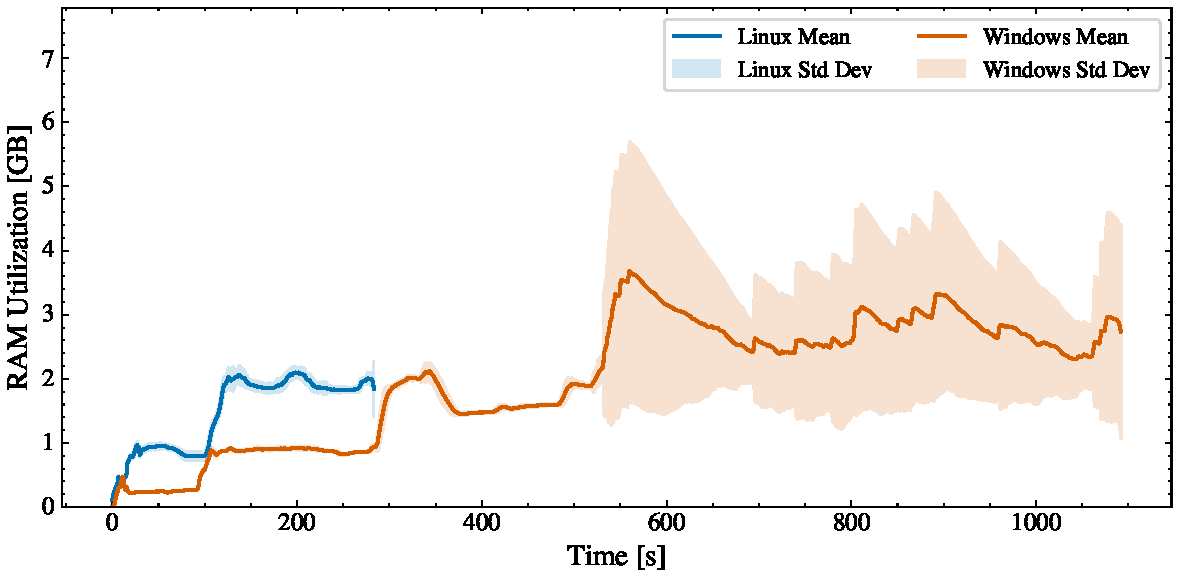
\includegraphics[width=\textwidth]{Messungen/WS_4T/ram_timeseries_combined.pdf}
\caption{Zeitlicher Verlauf der \acs{RAM}-Auslastung des Work-Stealing-Schedulers mit \acs{SSTF}-Priorisierung auf Linux und Windows bei vier Threads}
\label{fig:ws-4t-ram-ts}
\end{figure}

\subsection{Zehn Threads}
\begin{figure}[H]
\centering
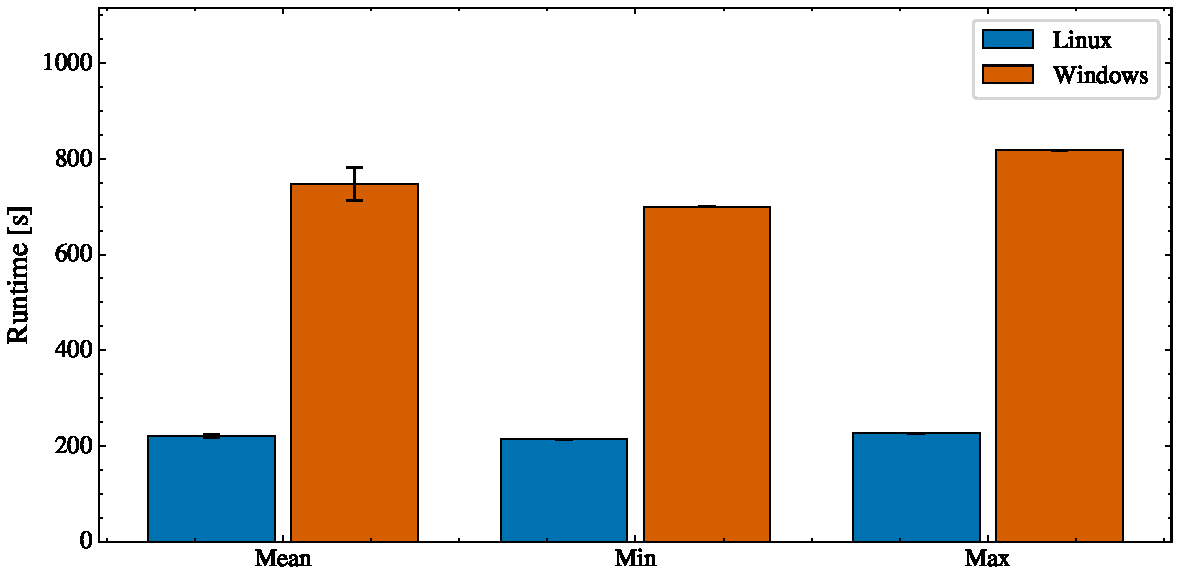
\includegraphics[width=\textwidth]{Messungen/WS_10T/runtime_bars_combined.pdf}
\caption{Laufzeiten des Work-Stealing-Schedulers mit \acs{SSTF}-Priorisierung auf Linux und Windows bei zehn Threads, dargestellt als Balkendiagramm mit Mittelwerten und Standardabweichungen aus 20 Messläufen}
\label{fig:ws-10t-runtime}
\end{figure}

\begin{figure}[H]
\centering
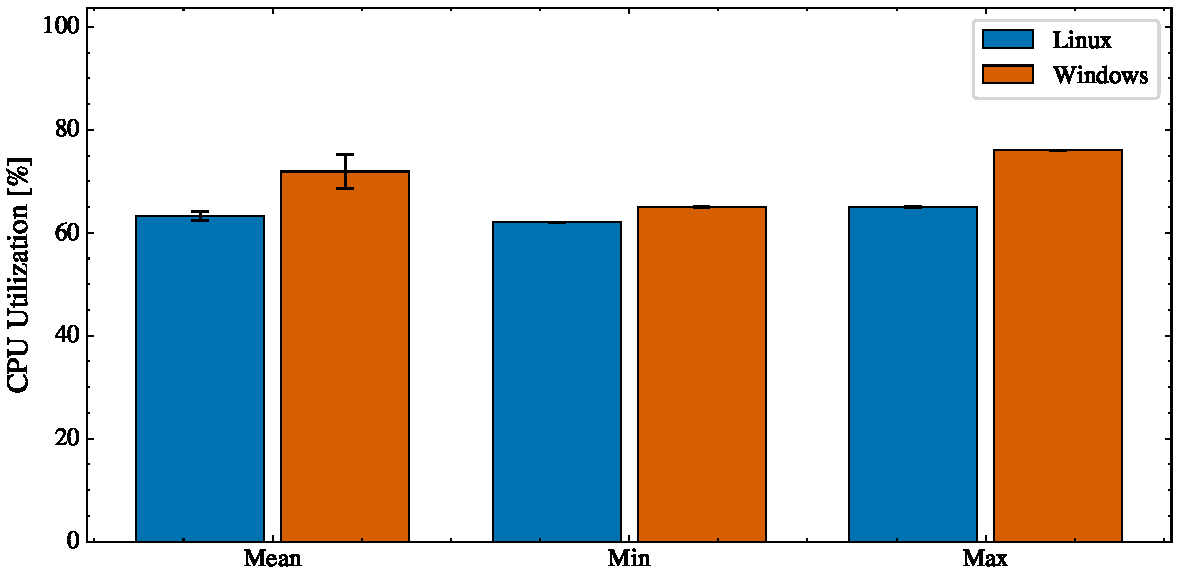
\includegraphics[width=\textwidth]{Messungen/WS_10T/cpu_bars_combined.pdf}
\caption{\acs{CPU}-Auslastung des Work-Stealing-Schedulers mit \acs{SSTF}-Priorisierung auf Linux und Windows bei zehn Threads, dargestellt als Balkendiagramm mit Mittelwerten und Standardabweichungen aus 20 Messläufen}
\label{fig:ws-10t-cpu}
\end{figure}

\begin{figure}[H]
\centering
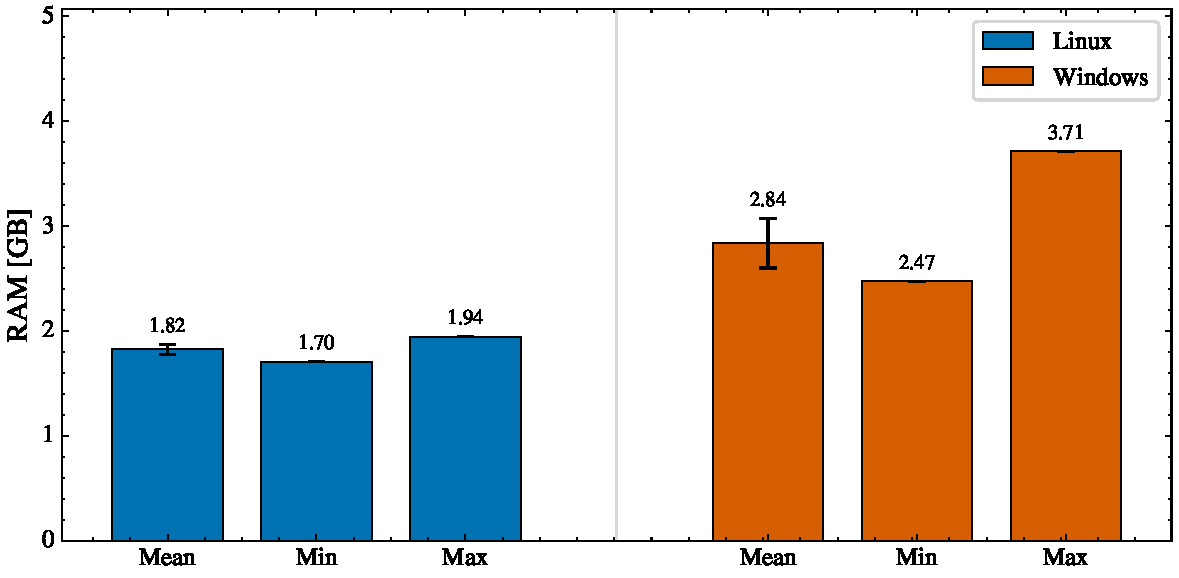
\includegraphics[width=\textwidth]{Messungen/WS_10T/ram_bars_combined.pdf}
\caption{\acs{RAM}-Auslastung des Work-Stealing-Schedulers mit \acs{SSTF}-Priorisierung auf Linux und Windows bei zehn Threads, dargestellt als Balkendiagramm mit Mittelwerten und Standardabweichungen aus 20 Messläufen}
\label{fig:ws-10t-ram}
\end{figure}

\begin{figure}[H]
\centering
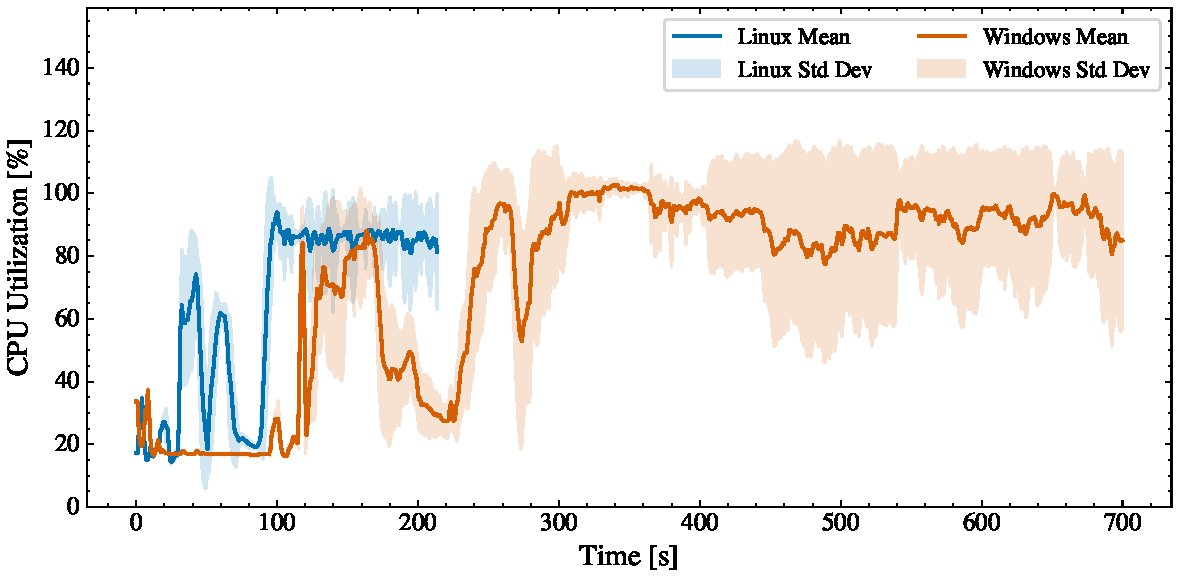
\includegraphics[width=\textwidth]{Messungen/WS_10T/cpu_timeseries_combined.pdf}
\caption{Zeitlicher Verlauf der \acs{CPU}-Auslastung des Work-Stealing-Schedulers mit \acs{SSTF}-Priorisierung auf Linux und Windows bei zehn Threads}
\label{fig:ws-10t-cpu-ts}
\end{figure}

\begin{figure}[H]
\centering
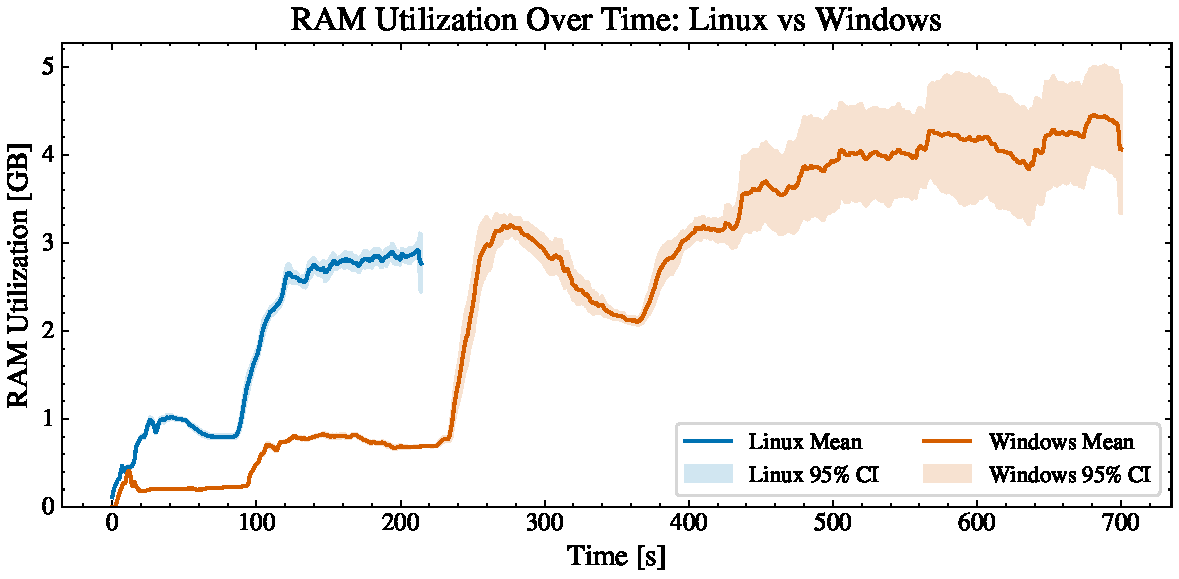
\includegraphics[width=\textwidth]{Messungen/WS_10T/ram_timeseries_combined.pdf}
\caption{Zeitlicher Verlauf der \acs{RAM}-Auslastung des Work-Stealing-Schedulers mit \acs{SSTF}-Priorisierung auf Linux und Windows bei zehn Threads}
\label{fig:ws-10t-ram-ts}
\end{figure}

\subsection{Vergleich}
\begin{figure}[H]
\centering
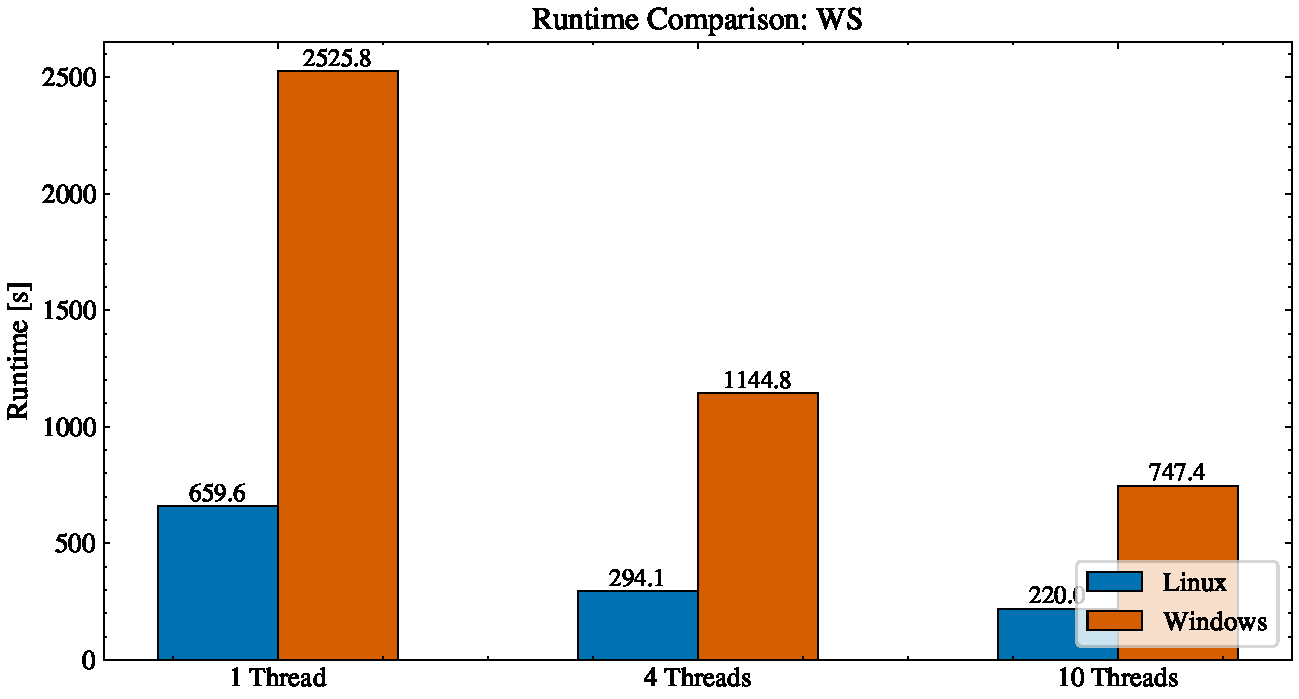
\includegraphics[width=\textwidth]{Messungen/Thread_Comparison/thread_ws_runtime.pdf}
\caption{Vergleich der Laufzeiten des Work-Stealing-Schedulers mit \acs{SSTF}-Priorisierung auf Linux und Windows über ein, vier und zehn Threads, dargestellt als Balkendiagramm mit Mittelwerten und Standardabweichungen aus 20 Messläufen}
\label{fig:ws-threadcmp-runtime}
\end{figure}

\begin{figure}[H]
\centering
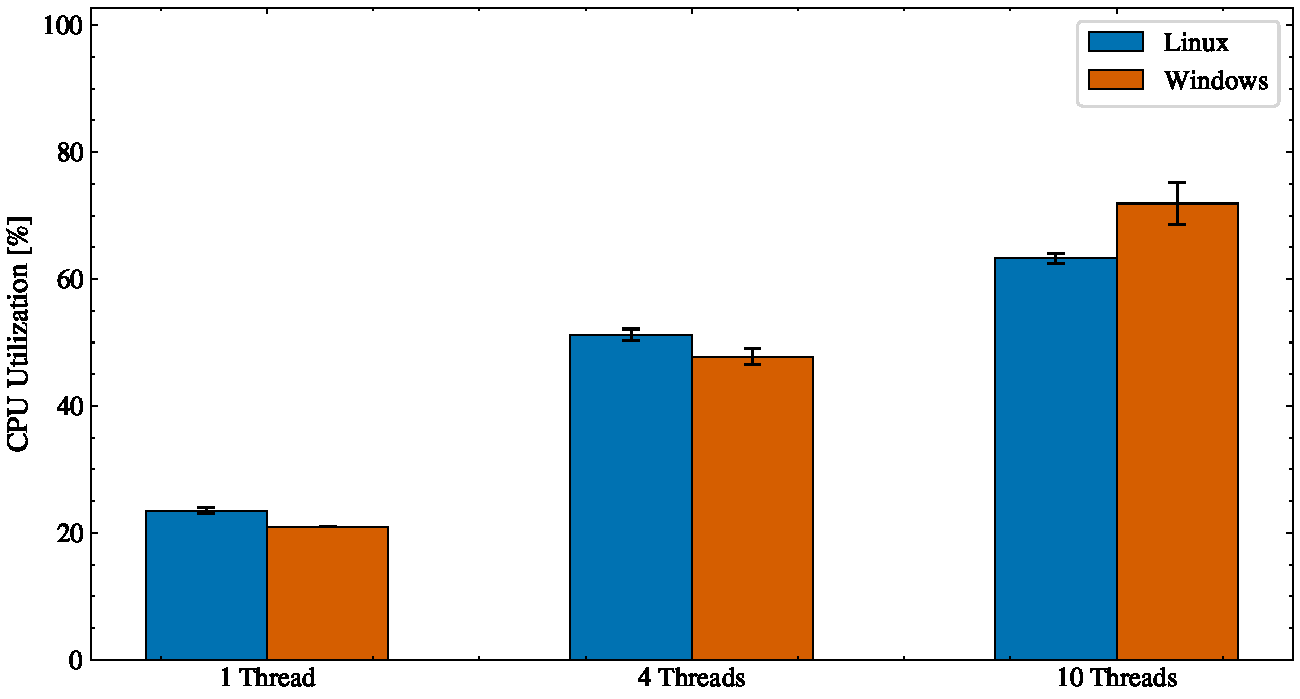
\includegraphics[width=\textwidth]{Messungen/Thread_Comparison/thread_ws_cpu.pdf}
\caption{Vergleich der \acs{CPU}-Auslastung des Work-Stealing-Schedulers mit \acs{SSTF}-Priorisierung auf Linux und Windows über ein, vier und zehn Threads, dargestellt als Balkendiagramm mit Mittelwerten und Standardabweichungen aus 20 Messläufen}
\label{fig:ws-threadcmp-cpu}
\end{figure}

\begin{figure}[H]
\centering
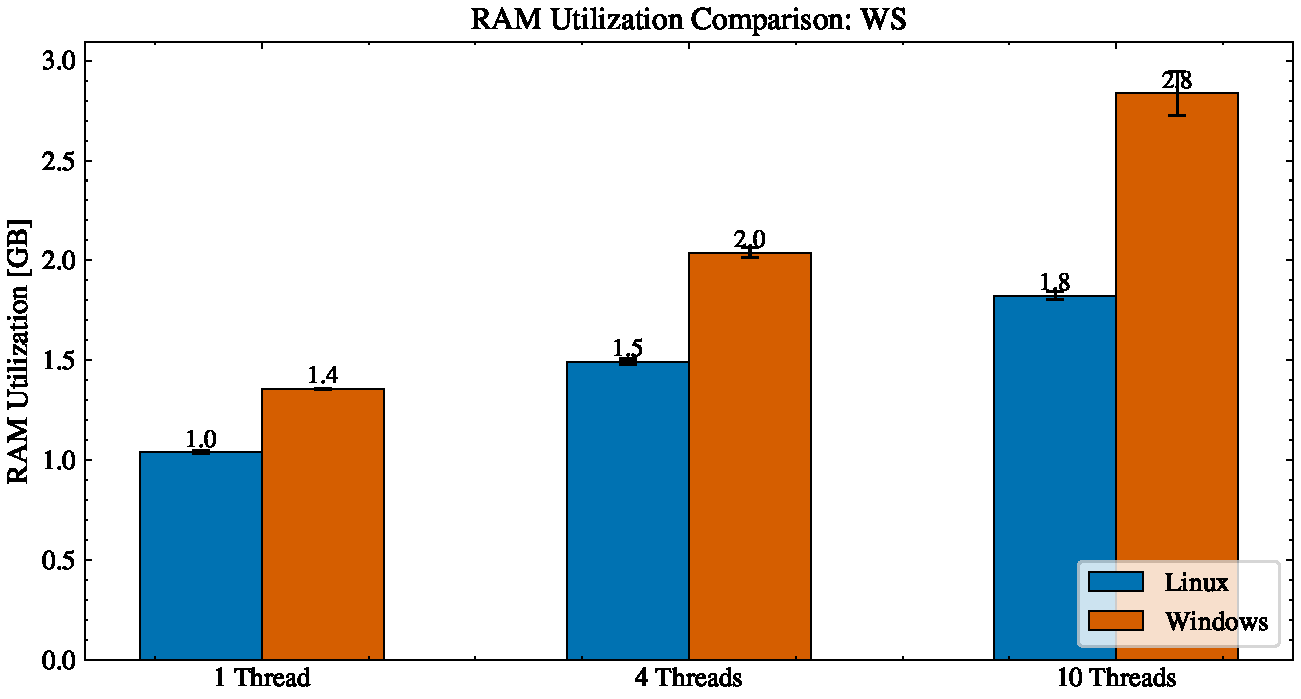
\includegraphics[width=\textwidth]{Messungen/Thread_Comparison/thread_ws_ram.pdf}
\caption{Vergleich der \acs{RAM}-Auslastung des Work-Stealing-Schedulers mit \acs{SSTF}-Priorisierung auf Linux und Windows über ein, vier und zehn Threads, dargestellt als Balkendiagramm mit Mittelwerten und Standardabweichungen aus 20 Messläufen}
\label{fig:ws-threadcmp-ram}
\end{figure}

\end{sloppypar}
